\documentclass[12pt,a4paper]{report} 

\usepackage[spanish]{babel} 
\usepackage{amsmath}
\usepackage{amsfonts}
\usepackage{amssymb}
\usepackage{graphicx}
\usepackage{listings}
\usepackage{xcolor}
\usepackage{url}
\usepackage{ucs}
\usepackage{epigraph}
\usepackage[utf8x]{inputenc}
\usepackage{afterpage}
\usepackage{appendix}
\usepackage{fancyhdr}
\usepackage{caption}
\usepackage{booktabs}

\newcommand{\HRule}{\rule{\linewidth}{0.5mm}}
\newcommand{\remo}{\textbf{Remo }}
\newcommand{\fudepan}{\textbf{FuDePAN}}
\newcommand{\FuD}{\textbf{FuD}}

\begin{document}

\pagenumbering{roman}

%---------Pagina principal. Caratula---------
\title{Estudio de la relación entre divergencia en el uso de codones sinónimos en virus-huésped y presencia de microRNA.}
\author{Riberi Franco G.}
\date{\today} 

\maketitle

%---------Subcaratula---------
\newpage
\thispagestyle{empty}

\begin{figure} [h]
	\begin{minipage}{.55\linewidth}
	\centering 
	
\includegraphics[scale=0.65]{image/unrc.jpg}
	\center{\textsc{\textbf{Universidad Nacional de R\'io Cuarto} \\ 
				\normalsize Departamento de Computaci\'on}
			}
	\end{minipage}
	\begin{minipage}{.45\linewidth}
	\centering 
	
\includegraphics[scale=0.65]{image/logo.jpg}
	\center{\textsc{\textbf{FuDePAN} \\ 
				\normalsize Fundación para el desarrollo de la programación en ácidos nucleicos}
			}
	\end{minipage}
\end{figure}

\vskip 1.1 cm

\begin{center} \textsc{\normalsize Trabajo Final} \end{center}
\begin{center} \textsc{\normalsize Licenciatura en Ciencias de la Computación} \end{center}

\noindent \HRule 
\begin{center} \large Estudio de la relación entre divergencia en el uso de codones sinónimos en virus-huésped y presencia de microRNA. \end{center} 

\HRule 
\vskip 2.5cm

\begin{center} 
\large \textbf{\emph{Autor:}}\\
\large Franco G. \textsc{Riberi}
\end{center}
\vskip 1.5cm

\begin{minipage}{0.35\textwidth}
\begin{center} 
\hspace*{1cm} \textbf{\emph{Directora:}}\\
\hspace*{1cm} Laura \\ \hspace*{1cm} \textsc{Tardivo}
\end{center} 
\end{minipage}
\begin{minipage}{0.55\textwidth}
\begin{center} 
\textbf{\emph{Co-Director:}} \\
Daniel \\ \textsc{Gutson}
\end{center}
\end{minipage}

%%---------------------Sintesis----------------------------------------------

\newpage
\thispagestyle{empty}
\begin{center} \LARGE \textbf{Resumen} \end{center}

\par El presente proyecto encuadra en una de las áreas de la Biología, conocida como Virología,
la cual estudia la acción de los virus en el organismo y cómo pueden ser aplicados ciertos fármacos para su tratamiento. 

\par El código genético está organizado en tripletes o codones (conjunto de tres nucleótidos que determinan un aminoácido). Al menos uno de estos tres nucleótidos puede ser distinto y sin embargo codificar para el mismo aminoácido, por lo cual se dice que el código genético esta \emph{degenerado}. Los tripletes que codifican para un mismo aminoácido se denominan \emph{sinónimos}.

\par Se conoce que cada especie tiene un uso de codones sinónimos característico que le permite optimizar la síntesis proteica. Para algunos organismos patógenos intracelulares, como los virus, existe una divergencia entre el uso de codones sinónimos utilizados por el virus y el huésped correspondiente. El origen de esa divergencia no está suficientemente esclarecido. 

\par En el presente trabajo se estudiará si la divergencia en el uso de codones sinónimos entre virus y huésped contribuye a disminuir la interferencia de los microRNA en la expresión de los RNA mensajeros de origen viral. De esa manera se contribuirá a comprender mejor la relación virus-huésped y la evolución viral.

\par Se desarrolló un software que realiza diversas comparaciones masivas entre secuencias de $_m$$_i$RNA y $_m$RNA, además de comparaciones a nivel estructural entre $_m$RNA. El software sigue una implementación distribuida, a través de la utilización de varios procesos que cooperan para realizar las tareas. Por otra parte, se implementaron diversas librerías con funcionalidades anexas, que se acoplan con otros paquetes de software relacionados con el área de estudio.

\vskip .5cm
\textbf{Palabras claves:} $_m$$_i$RNA, $_m$RNA, aminoácidos, nucleótidos, FuD, Remo, fideo.



%%-----------------Agradecimientos-------------------------------------------
\newpage
\thispagestyle{empty}
\chapter*{Agradecimientos} \addcontentsline{toc}{chapter}{Agradecimientos}


\rightline{\textit{A todos los que la presenten vieren y entendieren.}}
\rightline{\textbf{Inicio de las Leyes Org\'anicas.}}
\rightline{\textbf{Juan Carlos I.}}

\par \textbf{A Dios y la vida.}
\par Por haberme permitido llegar hasta este punto y haberme dado salud para lograr mis objetivos. \\

\par \textbf{A mi madre Alejandra Riberi.}
\par Por haberme inculcado la ética de trabajo y superación, por la motivación constante que me ha permitido ser una persona de bien, pero más que nada, por su amor. \\

\par \textbf{A mi padre Ariel Buffa.}
\par Por haberme apoyado en todo momento, por sus consejos, por el valor mostrado para salir adelante. \\

\par \textbf{A mi directora Laura Tardivo.}
\par Por dirigir este trabajo, por su constante ayuda, su predisposición, sus conocimientos y apoyo. \\

\par \textbf{A mi co-director Daniel Gutson.}
\par Por ser el mentor de este proyecto y quien confió mí para llevarlo adelante. Por su paciencia y dedicación. Por compartir su experiencia y conocimientos, tanto académicos como humanos. \\

\par \textbf{Al Dr. Daniel Rabinovich.}
\par Por su predisposición, dedicación y entusiamo. Por haberme otorgado la responsabilidad de llevar a cabo su intelecto. \\

\par \textbf{A los miembros de FuDePAN.}
\par Por estar siempre presentes, por el trabajo en conjunto. Especialmente al Lic. Emanuel Bringas por su constante apoyo y ayuda. \\

\par \textbf{Al Departamento de Computación.}
\par A todos los docentes que me capacitaron a lo largo de la carrera. Especialmente a Mg. Marcelo D. Arroyo por su colaboración cuando fue requerida. \\

\par \textbf{A mis compañeros y amigos.}
\par Quienes de diversas maneras estuvieron a mi lado durante este proceso compartiendo añecdotas, frustraciones y alegrías. \\

\par \textbf{A aquellas personas que ya no están a mi lado.}
\par Por haberme marcado de una u otra forma. \\

\par \textbf{A tí querido lector.}
\par Por tomarte el tiempo y la dedicación de leer este trabajo. \\

\vskip 1cm
\rightline{\textbf{Franco G. Riberi}}


%%--------------------Indice de Contenido------------------------------------
\index{INDICE}
\tableofcontents

%%-----------------------Indice de Figuras------------------------------------
\newpage
\listoffigures

%%--------------------Configuracion del Encabezado y Pie de pagina------------
\fancyhead{} 
\fancyhead[L]{\bfseries\rightmark}
\fancyfoot{} 
\fancyfoot[LE,RO]{\bfseries \thepage}
\fancyfoot[LO,RE]{Riberi Franco G.}
\renewcommand{\headrulewidth}{0.4pt}
\renewcommand{\footrulewidth}{0.4pt}
\pagestyle{fancy} 

%%---------------------------Contenido----------------------------------------
\pagenumbering{arabic}

\chapter*{Introducción}
\label{intro}

\epigraph{La vida sin pruebas y desafíos no sería provechosa, sino. ¿Como aprenderíamos?}%
{\textbf{Josue Alvarez. Guatemala }}

\par Debido al gran número de datos generados por los experimentos biológicos actuales, una nueva clase de híbridos ha surgido entre informáticos y biólogos. Los mismos se encargan de desarrollar métodos y programas para el análisis masivo de la información biológica. Dentro de esta línea, la \emph{Bioinformática} es considerada una de las disciplinas con mayor índice de expansión y crecimiento en la actualidad. 

\par No se puede abordar la Bioinformática sin describir inicialmente algunos conceptos elementales de la \emph{Biología}. En realidad son los biólogos y los bioquímicos quienes hicieron su primer acercamiento a la tecnología computacional como elemento fundamental para su trabajo diario. La tecnología proporciona un elemento teórico y las herramientas prácticas necesarias para que los científicos puedan explorar, analizar y establecer conclusiones al respecto.

\section*{La Biología}

\par \emph{La Biología} es aquella ciencia que estudia a los seres vivos, ya sean estos animales, plantas o seres humanos. Principalmente se preocupa de los procesos vitales de cada ser, tales como su nacimiento, desarrollo, muerte y procreación. Por lo que estudia el ciclo completo de los mismos\cite{curtis}. La palabra como tal, proviene del griego, \emph{bios} (vida) y \emph{logos} (estudio). Por lo tanto, la palabra en si, lo dice todo: \emph{Estudio de la vida}.

\par En particular, una de las áreas de aplicación de la Biología es la Virología, la cual estudia la acción de los virus y cómo pueden ser aplicados ciertos fármacos para su tratamiento.

\par Todos los seres vivos existentes sintetizan proteínas. De hecho, los tipos celulares (procariotas o eucariotas) están determinados por los tipos de proteínas que cada célula puede sintetizar. Por este motivo el material genético debe controlar los tipos y cantidades de proteínas que sintetiza una célula. Prácticamente todos los procesos biológicos dependen de la presencia o la actividad de proteínas. Dentro de las diversas funciones que desempeñan, se pueden mencionar las siguientes: función defensiva (crean los anticuerpos y regulan factores contra agentes extraños o infecciones), función reguladora (colaboran en la regulación de la actividad de las células, por ejemplo en la división celular), función estructural o de construcción (forman parte de las estructuras corporales suministrando el material necesario para el crecimiento y la reparación de tejidos y órganos del cuerpo), función energética (cuando el aporte de hidratos de carbono y grasas resulta insuficiente para cubrir las necesidades energéticas, las proteínas se emplean como combustible energético),  entre otras. 

\par Las \emph{proteínas}, también denominadas polipéptidos, están constituidas por cadenas de un surtido de sólo 20 \emph{aminoácidos}. A su vez, cada aminoácido se encuentra conformado por una sucesión de tres \emph{nucleótidos} consecutivos, los cuales se los denominan \emph{codón} o \emph{triplete}, y codifican a un determinado aminoácido. A pesar de ello, existen aminoácidos que son codificados por más de una combinación de codones, a los cuales se los conoce como \emph{codones sinónimos}. Desde una perspectiva computacional, esta secuencia de nucleótidos se trata de una cadena de caracteres pertenecientes al alfabeto de los 4 nucleótidos del \emph{DNA}(Ácido Desoxirribonucleico) conocidos como \emph{A}denina, \emph{C}itosina, \emph{G}uanina y \emph{T}imina. 

\par El nexo entre el DNA que se encuentra en el núcleo celular y las proteínas, que se encuentra en los ribosomas(citoplasma), lo conforma el RNA(Ácido Ribonucleico), aunque el mismo puede ser funcional por sí mismo (figura~\ref{fig}). Este flujo de la información que lleva a la producción de proteínas se denomina \emph{Dogma Central de la Biología}. 

\begin{figure}[h!]
    \centering
    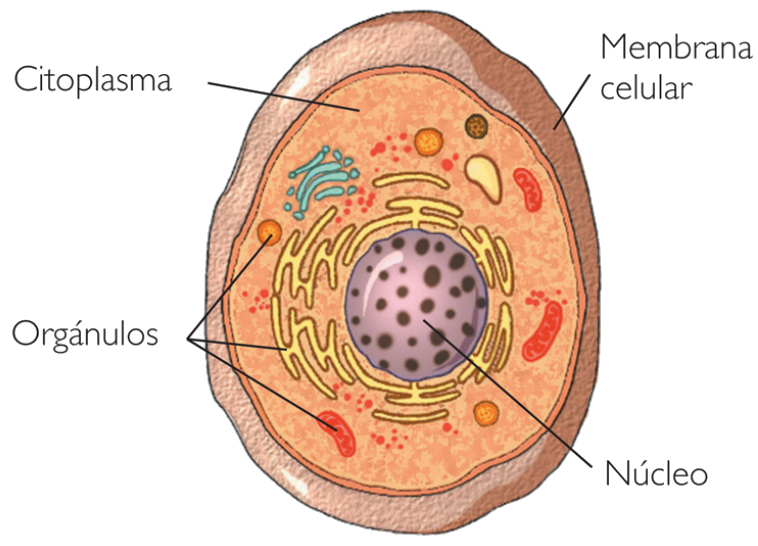
\includegraphics[scale=0.2]{image/celula.png}
    \caption{Estructura de un célula [1].}    
    \label{fig} 
\end{figure}    

\vskip 1cm
\par Básicamente, el DNA transfiere la información al RNA, el cual controla directamente la síntesis de proteínas. Este flujo es unidireccional, aunque existen excepciones. En este proceso entran en juego dos etapas importantes conocidas como \emph{transcripción} y \emph{traducción}. La transcripción es el proceso mediante el cual el RNA es sintetizado a partir de un molde de DNA, esto significa, que la información del DNA es reescrita, pero básicamente en el mismo lenguaje de nucleótidos. Por otro lado, la traducción es el proceso por el cual el RNA controla la síntesis de proteínas. En términos generales la información en el lenguaje de nucleótidos es traducida al lenguaje de aminoácidos\cite{genetica}. El proceso mencionado anteriormente se exhibe gráficamente en la figura~\ref{figIntro}.

\begin{figure}[h!]
    \centering
    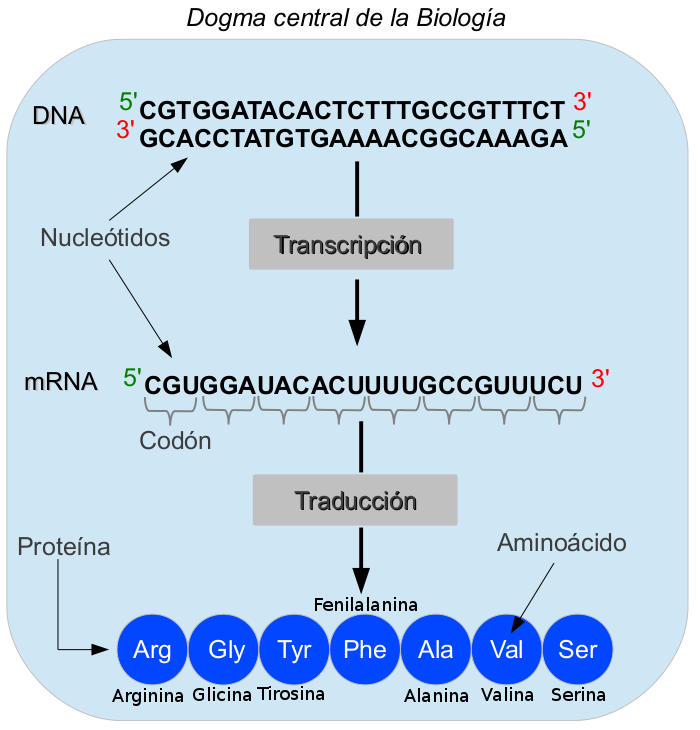
\includegraphics[scale=0.45]{image/resumen.png}
    \caption{Integrando conceptos iniciales [2].}
    \label{figIntro} 
\end{figure}    

\par Las secuencias mencionadas poseen diversos tamaños lo cual dificulta su procesamiento y análisis de forma manual. Las secuencias de proteínas contienen en promedio entre 100 y 5000 aminoácidos. Por otro lado, las secuencias de DNA son mucho más grandes que las de proteínas. Por ejemplo, el DNA de la bacteria E. Coli tiene 4.7 millones de nucleótidos y el del humano 3.3 billones.

\section*{La Bioinformática}
\par Si bien no existe una única definición, puede decirse que \emph{la Bioinformática} es la aplicación de las Ciencias de la Computación a la Biología Molecular. Este término hace referencia a campos de estudios interdisciplinarios muy vinculados, que requieren el uso o el desarrollo de diferentes técnicas que incluyen informática, matemática aplicada, estadística, Ciencias de la Computación, Inteligencia Artificial, Química y Bioquímica para solucionar problemas, analizar datos, o simular sistemas o mecanismos, todos ellos de índole biológica, y usualmente de nivel molecular. El núcleo principal de estas técnicas se encuentra en la utilización de recursos computacionales para solucionar o investigar problemas sobre escalas de tal magnitud que sobrepasan el discernimiento humano. 
\par Según la definición del Centro Nacional para la Información Biotecnológica (``National Center for Biotechnology Information'', NCBI por sus siglas en Inglés, 2001):
\begin{center}
\emph{``La Bioinformática es un campo de la ciencia en el cual confluyen varias disciplinas tales como: biología, computación y tecnología de la información. El fin último de este campo es facilitar el descubrimiento de nuevas ideas biológicas así como crear perspectivas globales a partir de las cuales se puedan discernir principios unificadores en biología.''}
\end{center}

\par Históricamente, el uso de las computadoras para resolver cuestiones biológicas comenzó con el desarrollo de algoritmos y su aplicación en el entendimiento de las interacciones de los procesos biológicos entre diversos organismos. La Biología Molecular es una ciencia rica en datos que crecen a tasas exponenciales\cite{NCBI}. Sin embargo, desde la perspectiva computacional la característica clave de los datos biológicos no es tanto su volumen sino su diversidad, heterogeneidad y dispersión, lo que impide o dificulta la explotación integrada de esta información.
\textbf{Los ``grandes volúmenes de datos'' se suelen citar como una de las características mas relevantes de la Bioinformática debido a sus tasas exponenciales de crecimiento.} Este crecimiento se debe en buena medida al desarrollo de nuevas tecnologías habiendo pasado del estudio de genes individuales a genomas completos y ahora a la interacción entre organismos.

\section*{\remo}
\par Luego de mencionar brevemente algunos conceptos importantes a continuación se presenta el trabajo titulado: \emph{``Estudio de la relación entre divergencia en el uso de codones sinónimos en virus-huésped y presencia de microRNA''}. El mismo tiene como principal objetivo contrastar una teoría postulada y encomendada por el Dr. Roberto Daniel Rabinovich\footnote{Miembro del Instituto Biomédico en Retrovirus y SIDA-INBIRS e investigador del Consejo Nacional de Investigaciones Científicas y Técnicas (CONICET), Buenos Aires, Argentina.}, que involucra principalmente la molécula de RNA. Dicho estudio surge como propuesta de la fundación FuDePAN\footnote{Fundación para el Desarrollo de la Programación en Ácidos Nucleicos, Córdoba, Argentina. \url{http://www.fudepan.org.ar/}}.

\par Se desea estudiar si la divergencia en el uso de codones sinónimos entre virus y huésped contribuye a disminuir la interferencia de los microRNA ($_m$$_i$RNA) en la expresión de los RNA mensajeros($_m$RNA) de origen viral. Los $_m$$_i$RNA son pequeñas moléculas codificadas en el DNA de las distintas especies que regulan la expresión de una gran fracción de las proteínas\footnote{Los $_m$$_i$RNA reconocen secuencias parcialmente complementarias en un $_m$RNA correspondiente, dando como resultando la inhibición de la traducción de dicho $m$RNA.}. Un $_m$RNA es un tipo particular de ácido ribonucleico monocatenario que contiene la información genética procedente del DNA(bicatenario) para utilizarse en la síntesis de proteínas. De esa manera se contribuirá a comprender mejor la relación virus-huésped y la evolución viral. Estos estudios tienen también una importancia potencial en la comprensión de la patogenia viral y en el desarrollo de herramientas terapéuticas como la terapia génica.

\par Para lograr tal objetivo se plantea desarrollar un software que, dadas ciertas secuencias de $_m$RNA y secuencias de $_m$$_i$RNA, permita determinar si la divergencia en el uso de codones sinónimos entre virus y huésped contribuye a disminuir la interferencia de los $_m$$_i$RNA en la expresión de los $_m$RNA de origen viral.

\par Dada la gran cantidad de datos a manipular y el tamaño de las secuencias, se requiere de un gran número de pequeños cálculos y comparaciones lo cual demanda un alto poder de cómputo. Por otro lado, para tener soporte de la ejecución distribuida se plantea utilizar el framework \emph{FuD}\footnote{FuDePAN Ubiquitous Distribution}\cite{clus09} sin tener que desarrollar específicamente esta funcionalidad y sin perder de vista el problema original.

\par Algunos motivaciones que llevaron a tomar la decisión de realizar el presente proyecto refieren a la posibilidad de enfrentarse con un problema real, de índole biológico, manipulando datos muy complejos tales como secuencias de DNA, secuencias de virus, entre otras. Por otro lado, de cierto modo, 
estos estudios pueden servir para contribuir a la investigación de temas relacionados con el área de la salud.

\par En el resto del documento se empleará el término \textbf{R-emo} o \remo para referirse al software desarrollado como solución planteada.

\section*{Estructura del Documento}
El documento esta compuesto por 8 capítulos, los cuales se detallan brevemente a continuación. 
\begin{itemize}
    \item \emph{Capítulo 1: La Biología,} describe los conceptos biológicos elementales necesarios para comprender el trabajo realizado. Algunos temas específicos quedan fuera del alcance de este documento, debido a la complejidad de los mismos, aunque no dejan de ser importantes.
    \item \emph{Capítulo 2: Descripción del Problema,} introduce el problema a resolver con una descripción general. 
    \item \emph{Capítulo 3: Metodología de Trabajo,} abarca la metodología de desarrollo seleccionada, detallando el modelo clásico y algunas consideraciones que se tuvieron en cuenta. Se describen las prácticas de software y herramientas empleadas.    
    \item \emph{Capítulo 4: Elicitación y Análisis de Requerimientos,} se describe brevemente la elicitación de requisitos y el análisis de los mismos, enunciando el estudio de las herramientas necesarias y búsqueda de datos mínimos.
    \item \emph{Capítulo 5: Diseño,} se menciona la arquitectura global de \remo y algunas consideraciones de diseño. 
    \item \emph{Capítulo 6: Implementación,} abarca detalles de implementación, representación de datos biológicos, el framework empleado para distribuir el trabajo, métricas de código, etcétera.
    \item \emph{Capítulo 7: Experimientación y Testing,} corresponde a las pruebas de \remo y las herramientas empleadas para tal fin.
    \item \emph{Capítulo 8: Conclusiones del Trabajo,} se detalla la conclusión del presente trabajo, los resultados, aportes y futuros desarrollos.    
\end{itemize}
A continuación de describe el presente trabajo.

%I Preliminares
\part{Preliminares}
   \chapter{La Biología}
\label{biologia}

\epigraph{Essentially, all models are wrong,
but some are useful.}%
{\textbf{George E. P. Box}}

\par Dado a que el presente informe corresponde a un trabajo de Ciencias de la Computación, sólo se presentarán algunas definiciones y conceptos biológicos elementales que brindarán al lector la capacidad de comprender los temas abordados en los próximos capítulos, ya que se utilizará un lenguaje al cual el mismo puede no estar habituado. No se abordarán rigurosamente todos los conceptos biológicos involucrados, quedando como tarea del lector interesado.

\section{Introducción a la Biología}

\par La \emph{Biología} es una ciencia que tiene como objeto de estudio a los seres vivos. Se ocupa tanto de la descripción de las características y los comportamientos de los organismos individuales como de las especies en su conjunto, así como de la reproducción de los seres vivos y de las interacciones entre ellos y el entorno. De este modo, trata de estudiar la estructura y dinámica funcional comunes a todos los seres vivos, con el fin de establecer las leyes generales que rigen la vida orgánica y los principios explicativos fundamentales de la misma\cite{curtis}. 

\subsection{Niveles de Organización Biológica}
\par Los \emph{niveles de organización biológica} son eslabones organizados de forma jerárquica, es decir, están organizados desde lo más simple hasta lo más complejo. Estos niveles se utilizan para clasificar la materia, de acuerdo a su tamaño y/o cantidad. A continuación se detallan los diferentes niveles de organización biológica:

\begin{itemize}
	\item \textbf{Nivel Atómico:} constituido por átomos. Aquellos elementos
			que forman la materia viva se conocen con el nombre
			de \emph{bioelementos}. Dentro de los mismos se encuentran 
			el carbono, el hidrógeno, el oxígeno, el nitrógeno, el
			azufre y el fósforo.

	\item \textbf{Nivel Molecular:} este nivel está formado por las
			moléculas que se originan al unirse dos o más átomos.
			Las moléculas que constituyen la materia viva se
			denominan \emph{biomoléculas}. Éstas pueden ser
			inorgánicas como el agua, las sales minerales o los
			gases, u orgánicas como los glúcidos, los lípidos, las
			proteínas y los ácidos nucleicos.

	\item \textbf{Nivel Celular:} se incluyen las células. Una célula
			es la menor porción de materia viva que conforman los organismo, dentro de 
			la cual tienen lugar todas las funciones vitales. Toda célula está
			formada por los niveles inferiores, el molecular y el
			atómico. La complejidad de este nivel es mucho mayor,
			ya que la célula es una unidad anatómica y funcional,
			esto significa que es la estructura más pequeña que
			podría sobrevivir por si misma.

	\item \textbf{Nivel Pluricelular:} refiere a la asociación de varias
			células que pueden llegar a constituir un organismo
			completo. Este nivel se puede subdividir en los
			siguientes subniveles: \emph{tejidos}, \emph{órganos}, \emph{sistemas} y \emph{aparatos}.  
            En conjunto forman el individuo pluricelular.

	\item \textbf{Nivel Población:} incluye al conjunto de individuos de
			la misma especie que viven en un lugar concreto y en
			un tiempo determinado pudiendo relacionarse entre sí.

	\item \textbf{Nivel Ecosistema:} abarca las relaciones que se
			establecen entre las poblaciones que viven en un
			determinado lugar y el ambiente en el que habitan. 
\end{itemize}

\par Como se puede observar, la Biología abarca muchas áreas de estudio. El presente trabajo se encuentra a nivel molecular, por lo cual a continuación se desarrollarán conceptos pertinentes a este nivel, el cual es conocido dentro de la jerga como \textit{Biología Molecular}.

\subsection{Moléculas Orgánicas y Macromoléculas}
\label{molOrg}

\subsubsection{Moléculas Orgánicas}
Las moléculas orgánicas pueden definirse como aquellas que contienen carbono y se encuentran en los seres vivos. Hay dos tipos de moléculas orgánicas básicas:
\begin{enumerate}
    \item \textbf{Nucleótidos:} corresponden a pequeñas moléculas constituyentes de macromoléculas
    de mayor complejidad tales como los ácidos nucleicos. Un nucleótido está formado por un azúcar, un
    fosfato y una base nitrogenada como se observa en la figura~\ref{nucleotido}. Además de su papel en la
    formación de ácido nucleicos, tiene una función independiente y vital para la vida celular.
    Cuando un nucleótido se modifica por la unión de dos fosfatos, se convierte en un transportador de
    energía, la cual es necesaria para que se produzcan numerosas reacciones químicas celulares.

    Las bases nitrogenadas se clasifican en:
	\begin{itemize}
	    \item \textit{Bases nitrogenadas purínicas:} encontramos la Adenina(\textbf{A}) y Guanina(\textbf{G}).
		\item \textit{Bases nitrogenadas pirimidínicas:} encontramos la Timina(\textbf{T}), Citocina(\textbf{C}) y Uracilo(\textbf{U}).
		\item \textit{Bases nitrogenadas isoaloxacínicas:} encontramos la Flavina(\textbf{F}).
	\end{itemize}
	Las bases \textbf{A}, \textbf{G} y la \textbf{C} forman parte del DNA y RNA. La base \textbf{T} sólo forma parte del DNA, y en contrapartida, la base \textbf{U} sólo forma parte del RNA.	
    \begin{figure} [!h]       
    	    \hspace*{4cm}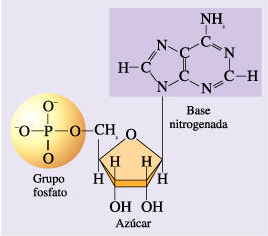
\includegraphics[width=2.5209in,height=2.000in]{image/nucleotido.png}
    		\caption{Estructura de un Nucleótido [4].}			
    		\label{nucleotido}
    \end{figure}				

    \item \textbf{Aminoácidos:} son las unidades estructurales que conforman las proteínas y sirven como materia prima para la formación de una gran variedad de compuestos nitrogenados con actividad fisiológica de vital importancia para la vida. Existen 20 aminoácidos que se exhiben en la figura~\ref{aminoac} y que  tienen codones específicos\footnote{Recordemos que un codón es un conjunto de tres nucleótidos.} en el código genético (figura ~\ref{codGen}). La unión de varios aminoácidos da lugar a cadenas llamadas polipéptidos o simplemente péptidos, que se denominan \emph{proteínas} cuando la cadena polipeptídica supera los 50 aminoácidos.
    	\begin{figure}[!h]
    		\hspace*{1cm}\begin{tabular}{| l | c | c |}
				\hline
				{\bf Nombre} & {\bf Ab. 3 letras} & {\bf Ab. 1 letra} \\
				\hline
				\hline
				Alanine (Alanina) & Ala & A\\\hline
				Arginine (Arginina) & Arg & R\\\hline
				Asparagine (Asparagina) & Asn & N\\\hline
				Aspartic acid (Aspartato) & Asp & D\\\hline
				Cytesine (Cisteína) & Cys & C\\\hline
				Glutamic acid (Ácido glutámico) & Glu & E\\\hline
				Glutamine (Glutamina) & Gln & Q\\\hline
				Glycine (Glicina) & Gly & G\\\hline
				Histidine (Histidina) & His & H\\\hline
				Isoleucine (Isoleucina) & Ile & I\\\hline
				Leucine (Leucina) & Leu & L\\\hline
				Lysine (Lisina) & Lys & K\\\hline
				Methionine (Metionina) & Met & M\\\hline
				Phenylalanine (Fenilalanina) & Phe & F\\\hline
				Proline (Prolina) & Pro & P\\\hline
				Serine (Serina) & Ser & S\\\hline
				Threonine (Treonina) & Thr & T\\\hline
				Tryptophan (Triptófano) & Trp & W\\\hline
				Tyrosine (Tirosina) & Tyr & Y\\\hline
				Valine (Valina) & Val & V\\\hline										
			\end{tabular}
			\caption{Tabla de representación de Aminoácidos [2].}
			\label{DnaRna}
			\label{aminoac}
		\end{figure}

		\begin{figure}[h]		
			\hspace*{2cm} 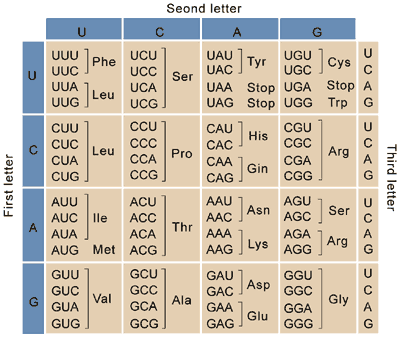
\includegraphics[width=3.9in, height=2.8in]{image/gencode.png}
			\caption{Código Genético [5].}
			\label{codGen}			
		\end{figure}	
\end{enumerate}

\vskip 2.5cm
\subsubsection{Macromoléculas}
Las macromoléculas son estructuras biológicas conformadas por un determinado número de moléculas orgánicas. Dentro de las macromoléculas podemos encontrar: \emph{Glúsidos}, \emph{Lípidos}, \emph{Proteínas} y
\emph{Ácidos Nucleicos}. Las dos primeros escapan al presente trabajo, por lo cual se deja a criterio del lector su investigación.

\begin{itemize}
	\item \textbf{Ácidos Nucleicos:} están conformados por secuencias de nucleótidos específicos, que son
    utilizados por todos los organismos para almacenar su información genética. La misma, está codificada
    mediante sucesivos codones, los cuales están conformados por tripletes de nucleótidos que codifican (traducen) a un determinado aminoácido. Existen dos tipos principales de ácidos nucleicos:
    	\begin{enumerate}
			\item \textbf{DNA (Ácido Desoxirribonucleico):} almacena y transmite la información    
			genética para el desarrollo y el funcionamiento de los organismos vivos y de algunos virus, la cual se hereda de generación en generación. Está formado por una doble cadena de nucleótidos, donde las dos hebras están unidas a través de las bases complementarias (respetando una estructura helicoidal) según el modelo propuesto por Watson\footnote{James Dewey Watson, biólogo estadounidense. Premio Nobel en Medicina.} y Crick\footnote{Francis Harry Compton Crick (1916-2004), físico, biólogo molecular y  neurocientífico británico. Premio Nobel en Medicina.} en 1953 (ver apéndice ~\ref{modelo}). El DNA contiene azúcares y fosfatos en su exterior y las bases en su interior. 
    		La doble hélice le proporciona al DNA una increíble estabilidad y permanencia. Las dos cadenas polinucleótidas se disponen en direcciones opuestas, es decir son antiparalelas, lo que significa que el extremo denominado \emph{5'} de una cadena se ubica en oposición al extremo denominado \emph{3'} de la otra cadena, tal como se exhibe en la figura~\ref{extremos}.

    		\begin{figure} [h]
				\begin{center}
					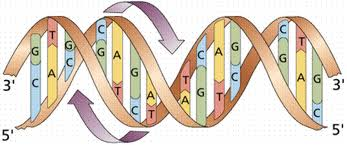
\includegraphics[width=2.9209in,height=1.0000in]{image/extremos.jpg}
					\caption{DNA: cadenas antiparalelas [6].}				
					\label{extremos}
				\end{center}
			\end{figure}	

			\item \textbf{RNA (Ácido Ribonucleico):} consiste en una hebra de cadena simple, la cual usualmente es trascripta a partir de una porción de DNA y se utiliza posteriormente en la célula para la síntesis de proteínas (sección~\ref{sintesisProteica}).			
		\end{enumerate}				
	Aunque el DNA y RNA son muy semejantes, desempeñan papeles biológicos muy diferentes. El DNA es el constituyente principal de los cromosomas de las células y es el portador del mensaje genético. En cambio, en RNA tiene como función transcribir el mensaje presente en el DNA y traducirlo a las proteínas. 
    Además, el DNA se encuentra principalmente en el núcleo celular, mientras que el RNA se encuentra en el citoplasma, donde se produce la síntesis de proteínas.							
	Otra diferencia entre estos dos tipos de ácidos nucleicos radica en las propias diferencias naturales existentes entre sus nucleótidos y residen en el tipo azúcar (ribosa en el caso del RNA y desoxirribosa en el caso del DNA) y las bases nitrogenadas características de cada uno.
	Otro rasgo a destacar, es que a pesar de que en la mayoría de las especies el DNA lleva la información genética, existen casos donde el RNA sirve como material genético (por ejemplo algunos virus tales como el TMV\footnote{Virus del mosaico del tabaco.}). En la figura~\ref{DnaRna} se puede observar gráficamente la cadena doble característica del DNA (parte derecha de la figura) y la cadena simple del RNA (parte izquierda de la figura).	
					
	\begin{figure} [h]
		\begin{center}
		   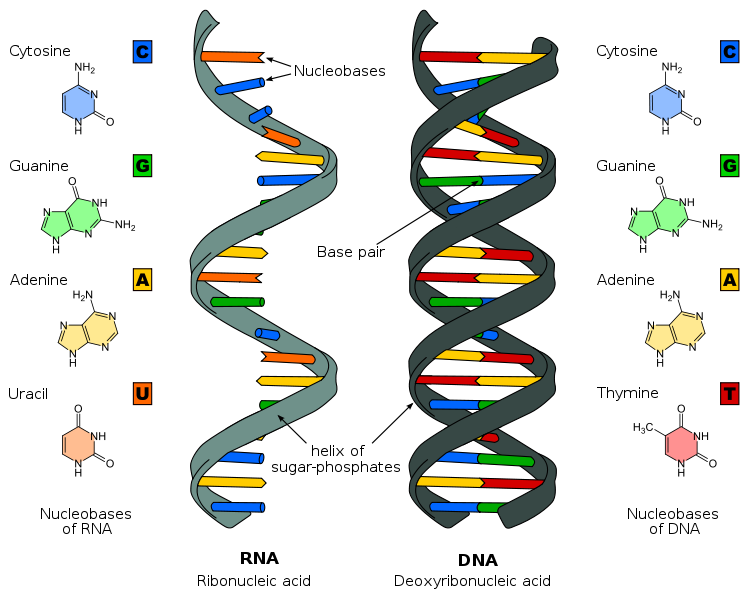
\includegraphics[width=5.0209in,height=4.0000in]{image/ARN-ADN.png}
		   \caption{Representación gráfica del RNA y DNA [7].}			
		   \label{DnaRna}
		\end{center}
	\end{figure}	

	\item \textbf{Proteínas:} son las moléculas más abundantes y de máxima importancia biológica porque la ordenación de los distintos monómeros\footnote{Un monómero es una molécula de pequeña masa muscular que unida a otros monómeros por medio de enlaces químicos forman macromoléculas denominadas \emph{polímeros}.} en su estructura permite que sean utilizados como vehículo de la información celular.
	Están formadas por secuencias de aminoácidos específicas (se considera proteína a aquellas cadenas de aminoácidos enlazados cuyo peso molecular es superior a 6000 Daltons), que adoptan una conformación tridimensional determinada debido a las interacciones electrostáticas existentes entre los residuos de sus aminoácidos constituyentes. 
	La estructura molecular de las proteínas (figura~\ref{proteina}) tiene varios niveles de organización, al igual que los ácidos nucleicos. La \textit{estructura primaria} consiste en una secuencia de aminoácido.
    A través de las interacciones entre los aminoácidos vecinos, una cadena polipeptídica se pliega y se enrosca para formar una \textit{estructura secundaria}. Las estructuras secundarias interactúan y se pliegan adicionalmente para forma lo que se conoce como \textit{estructura terciaria}, que es la forma completa, tridimensional de la proteína. Finalmente, algunas proteínas consisten en dos o más cadenas polipeptídicas que se asocian para producir una \textit{estructura cuaternaria.} 
	\par Las proteínas no son capaces de portar información genética y transmitirla a la descendencia, como ya se mencionó, este papel es realizado por los ácidos nucleicos, en particular por el DNA. Éste necesita de las proteínas para replicarse, y a su vez, las proteínas necesitan de la información que provee el DNA su síntesis.					
	\par Desde el punto de vista funcional, juegan un rol fundamental, dado que todo proceso biológico
	depende de la presencia y/o actividad de estas sustancias. Son proteínas casi todas las \textit{enzimas}
	(catalizadores de reacciones químicas en los organismos), \textit{hormonas} (reguladores de actividades celulares), \textit{hemoglobina} (transporte de sangre), \textit{anticuerpos} (encargados de acciones de defensa natural contra infecciones o agentes extraños), entre otras.
	\par Cabe destacar que existe una relación colineal con los genes\footnote{Un gen se define como un factor hereditario que determina una característica.}, es decir, hay una correspondencia directa entre la secuencia de nucleótidos del DNA y la secuencia de aminoácidos de una proteína. El concepto de colinealidad sugiere que el número de nucleótidos de un gen debería ser proporcional al número de aminoácidos de la proteína codificada por ese gen.

    \begin{figure} [h]
	    \begin{center}
		    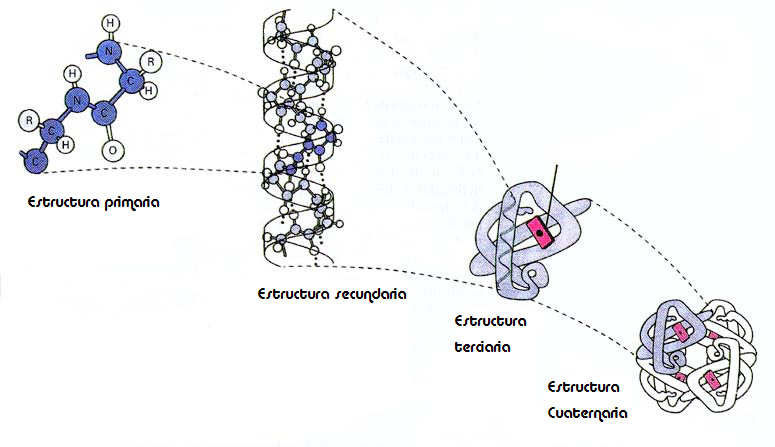
\includegraphics[width=5.7209in,height=2.7000in]{image/estructuraProteina.png}
		    \caption{Estructura molecular de las proteínas [8].}
		    \label{proteina}
	    \end{center}
    \end{figure}	
\end{itemize}

Las primeras investigaciones a cerca del material genético y su relación con DNA y proteínas mostraron que un cromosoma\footnote{Se denomina cromosoma a cada uno de los pequeños cuerpos en forma de bastoncillos en que se organiza la cromatina del núcleo celular durante las divisiones celulares. La cromatina es el conjunto de DNA y proteínas que se encuentra en el núcleo de las células.} estaba formado por DNA y proteínas en cantidades aproximadamente iguales. Por lo cual, ambos eran candidatos para desempeñar el papel de material genético. Las proteínas parecían ser la opción correcta dada su mayor complejidad química, aunque esta hipótesis era lógica fue errónea. 
El descubrimiento de la sustancia que puede transmitir características genéticas de una célula a otra resultó de los estudios con neumococos\footnote{Bacterias que causan la neumonía.}\cite{curtis}.

\subsection{Estructura del DNA}
\begin{itemize}
	\item \emph{Estructura Primaria}: consiste en una cadena de nucleótidos unidos entre sí por uniones fosfodiéster. 
	\item \emph{Estructura Secundaria}: se relaciona con su configuración tridimensional (su 		
				estructura helicoidal básica). Esta estructura puede adquirir diversas configuraciones de acuerdo con su secuencia de bases y las condiciones en que
				se encuentran.
				Dentro de las mismas, encontramos la estructura \textbf{B-DNA}, la cual depende de que la molécula esté rodeada por abundante agua, además es la estructura más estable. Por otro lado, la estructura \textbf{A-DNA} la cual se presenta cuando la cantidad de agua es menor. Y por último, la estructura \textbf{Z-DNA} la cual se genera cuando
				el DNA es colocado en una solución de alta concentración salina. Las estructuras mencionadas se exhiben en la figura~\ref{estrucDNA}.
\end{itemize}

\begin{figure} [h]
  		\hspace*{2cm}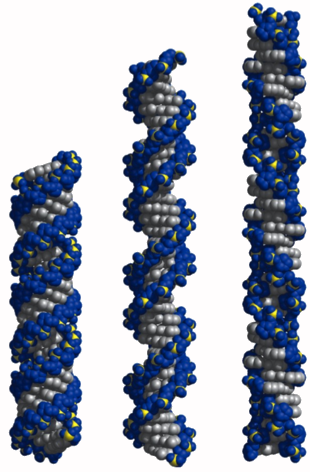
\includegraphics[width=3.5209in,height=3.5000in]{image/estructuraSecDNA.png}
   		\caption{Estructuras secundarias del DNA. A-DNA, B-DNA y Z-DNA de izquierda a derecha respectivamente [9].}
   		\label{estrucDNA}
\end{figure}	

\subsection{Replicación de DNA}
\par Consiste en el proceso a través del cual una célula duplica su DNA antes de dividirse. Dicho proceso es muy complejo, tal es así, que un componente defectuoso puede producir síntomas patológicos graves. 
\par La replicación es fundamental para el funcionamiento y mantenimiento de la célula y ocurre sólo una vez en cada generación celular, resultando esencial en la duplicación de los cromosomas.

\vskip 0.5cm
\noindent \textbf{Replicación semicorservativa}
\vskip 0.025cm

Básicamente la molécula de DNA se abre por el medio, separándose por bases apareadas (A=T; C=G) al nivel de los puentes de hidrógeno. A medida que las dos cadenas se separan, actúan como moldes o guías, es decir, cada una dirige la síntesis de una nueva cadena complementaria, utilizando las materias primas de la célula (figura~\ref{semi}).
Este modelo de replicación se conoce como \textit{replicación semiconservadora}, dado que se conserva la mitad de la molécula original en cada nueva cadena hija. Esto es, si hay una \textbf{T} presente en la cadena original, solamente puede ubicarse una \textbf{A} en el lugar correspondiente en la nueva cadena, de igual forma, una \textbf{G} sólo se apareará con una \textbf{C}, y así sucesivamente. Así, cada cadena forma una copia de su cadena complementaria original y se producen dos réplicas exactas de la molécula.

\begin{figure} [h]
		\hspace*{4.5cm}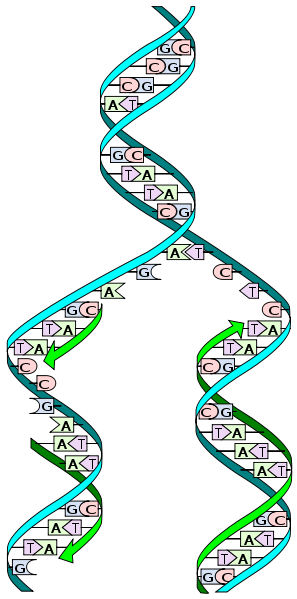
\includegraphics[width=2.1209in,height=3.5000in]{image/replicacionSemiconservativa2.png}
		\caption{Replicación semiconservativa [10].}		
		\label{semi}
\end{figure}				

El proceso real de replicación en un poco más complejo que la replicación semiconservadora. La replicación del DNA requiere de diferentes enzimas, las cuales catalizan un paso particular del proceso. 

\subsection{Del DNA a la Proteína}
\subsubsection{El Dogma Central de la Biología}
\par Este dogma\footnote{Un dogma es una proposición que se asigna como cierta e innegable, no sujeta a prueba de veracidad.} proclamado por Francis Crick en 1956 indica que la información fluye en una única dirección, es decir, el DNA transfiere la información al RNA, el cual controla directamente la síntesis de proteínas (figura ~\ref{dogma}). Así, el genotipo\footnote{El genotipo es la totalidad de la información genética que posee un organismo en particular, en forma de DNA. También puede definirse como el conjunto de genes de un organismo.} determina el fenotipo\footnote{Se denomina fenotipo a la expresión del genotipo en función de un determinado ambiente. También puede definirse como el conjunto de rasgos de un organismo.}, dictando la composición de las proteínas. Sin embargo, estas últimas no alteran al genotipo, es decir, las proteínas no envían instrucciones de regreso. 
\par Este dogma posee algunas excepciones, la principal de ellas es el proceso conocido como \textit{transcripción inversa}, en el cual la información codificada por cierto virus que contienen RNA se transcribe al DNA por la acción de la enzima transcriptasa inversa. 
\par El hecho de que la información fluya del DNA al RNA, y de éste a las proteínas suministró cierta confirmación de la teoría darwinista de la evolución. Según esta teoría, la selección natural actúa sobre las variaciones heredables encontradas en el DNA\cite{curtis}.

%Transcripcion
% Proceso mediante el cual el RNA es sintetizado a partir de un molde de DNA, esto es, la informacion del DNA es reescrita, pero básicamente en el mismo lenguaje de nucleṕtidos.

% El proceso por el cual el RNA controla la síntesis de proteinas se llana traudccion porque la informacion en el lenguaje de nucleotidos es traducida en nformacion en lenguaje de aminoaciodos.

\begin{figure} [h]
	\hspace*{3cm}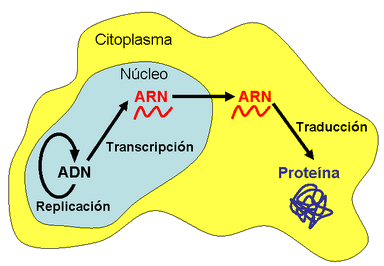
\includegraphics[width=2.6209in,height=1.4000in]{image/rel.png} %rel.png
	\caption{El Dogma Central [11].}	
	\label{dogma}
\end{figure}				

Existen diferentes clases de RNA que desempeñan diferentes funciones como intermediarios entre los pasos que llevan del DNA a las proteínas. Éstos son:
\begin{itemize}
	\item RNA mensajero\textbf{($_m$RNA):} se encuentra tanto en el núcleo como en el citoplasma de una célula. Su función es portar el código genético para las proteínas, es decir, transportan las instrucciones de codificación de las proteínas desde el DNA hasta el ribosoma. Después de unirse al ribosoma, una molécula de $_m$RNA especifica la secuencia de los aminoácidos de la proteína y proporciona un molde para unirlos.
	\item RNA de transferencia\textbf{($_t$RNA):} se encuentra sólo en el citoplasma. Sirve como enlace entre la secuencia codificante de nucleótidos de $_m$RNA y la secuencia de aminoácidos de una cadena polipeptídica. Cada $_t$RNA se une a un tipo particular de aminoácido y ayuda a incorporarlo a una cadena polipeptídica.
	\item RNA ribosómico\textbf{($_r$RNA):} se encuentra sólo en el citoplasma. Es un componente estructural y funcional del ribosoma (sitio de ensamblaje de proteínas).
	\item RNA interferente pequeño\textbf{($_s$$_i$RNA)} y microRNA\textbf{($_m$$_i$RNA)}: son moléculas muy pequeñas presentes en las células eucariotas que inhiben específicamente la expresión de genes a nivel post-transcripcional, en respuesta a la presencia de RNA de doble hebra que proviene de la propia célula ($_m$$_i$RNA) o del exterior de la misma (RNA pequeños de interferencia o $_s$$_i$RNA). Particularmente, los $_m$$_i$RNA son pequeños RNA codificados en el DNA de las distintas especies que regulan la expresión de una gran fracción de las proteínas. Para que esto ocurra, el debe encontrar nucleótidos complementarios (la unión se ve favorecida si estos nucleótidos no se ven comprometidos en la estructura secundario de la molécula) en el $_m$RNA blanco. %Recientemente se ha demostrado que, no sólo la unión de los $_m$$_i$RNA a la región no codificante puede disminuir la expresión proteica, sino que se han registrado uniones a regiones codificantes que producen una regulación negativa.
\end{itemize}

\subsubsection{Transcripción}
En este proceso las secuencias de DNA son copiadas a RNA mediante una enzima llamada RNA polimerasa. Dicha enzima sintetiza un RNA que mantiene la información de la secuencia del DNA. De esta manera, la transcripción del DNA también podría llamarse síntesis del RNA. En términos generales es la síntesis de una molécula de RNA a partir de un molde de DNA.

La transcripción es un proceso muy parecido a la replicación del DNA pero existe una diferencia fundamental relacionada con la longitud del molde empleado. Durante la replicación se copian todos los nucleótidos del molde de DNA pero durante la transcripción sólo pequeñas porciones de DNA se transcriben a RNA (casi siempre un único gen o a lo sumo algunos genes). Por lo cual, la transcripción es un proceso selectivo, es decir, se transcriben genes individuales sólo cuando se requieren sus productos. Esta selectividad implica la identificación de genes individuales y su transcripción en el momento y lugar adecuado.

\par Las moléculas de RNA son largas copias de secuencias de una cadena simple de DNA pero, a diferencia de las moléculas de DNA, se encuentran en su mayoría como moléculas de cadena única. Cada nueva molécula de RNA se copia de una de las dos cadenas de DNA (la cadena molde, la otra cadena restante de la doble hélice en general no se transcribe) según el mismo principio de apareamiento de bases que gobierna la replicación del DNA, como se puede observar en la figura~\ref{transcripcion}. 

\begin{figure} [h]
	\hspace*{3.5cm}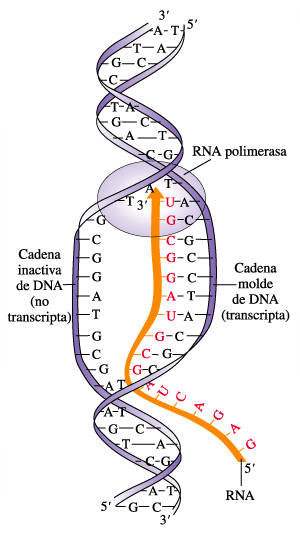
\includegraphics[width=2.2209in,height=3.5000in]{image/transcripcion.jpg}
	\caption{Representación esquemática de la transcripción del RNA [12].}
	\label{transcripcion}
\end{figure}				

% El proceso conocido como \textit{transcripción}, es catalizado por la enzima \textit{RNA polimerasa}, la cual opera de la misma forma que la DNA polimerasa, moviéndose en dirección 3' a 5' a lo largo de la cadena molde de DNA, sintetizando una nueva cadena complementaria de nucleótidos en la dirección 5' a 3'. Así la cadena de RNA es antiparalela a la cadena molde de DNA de la cual es transcripta.
% \par La RNA polimerasa, a diferencia de la DNA polimerasa, no requiere cebador para comenzar la síntesis de RNA, ya que es capaz de iniciar una nueva cadena uniendo dos ribonucleícos.

% \par En \textbf{procariotas}, cuando se inicia la transcripción, la RNA polimerasa se une al DNA en una secuencia específica denominada \textit{secuencia promotora o promotor}, abre la doble hélice en una pequeña región y así quedan expuestos los nucleótidos de una secuencia corta de DNA. Luego, la enzima va añadiendo ribonucleótidos, moviéndose a lo largo de la cadena molde, desenrrollando la hélice y exponiendo así nuevas regiones con las que se aparearán los ribonucleótidos complementarios. El proceso de elongación de la nueva cadena de RNA continua hasta que la enzima encuentra otra secuencia especial en el transcripto naciente, la \textit{señal de terminación}. En muchos casos esta señal esta dada por la estructura secundaria del RNA. En este momento, la polimerasa se detiene y libera a la cadena de DNA molde y a la recién sitetizada cadena de RNA. Sólo una cadena es transcripta por gen, la RNA polimerasa debe saber cual copiar, la responsable de esta decisión es la secuencia promotora.

% \par En \textbf{eucariotas} el proceso es similar, aunque primero se transcribe un $_p$$_r$$_e$$_-$$_m$RNA a partir del DNA, el cual se procesa para obtener un RNA maduro. La unión de la RNA \textit{polimesasa} a una secuencia de nucleótidos determinada, (el promotor), requiere la unión previa de factores proteicos. Existen tres RNA \textit{polimerasa}: I, II y III. La RNA polimerasa I transcribe los genes de los $_r$RNA grandes, la polimerasa II transcribe los genes que se tradicirán a proteínas, y la polimerasa III transcribe una variedad de RNA pequeños. 

\par La mayor parte de los transcriptos sufren un procedimiento posterior a la transcripción antes de dejar el núcleo e ingresar al citoplasma llamado \textit{splicing}.
\par En conclusión, el RNA transcripto a partir del DNA es la copia activa de la información genética.


\subsubsection{Traducción} 
\label{sintesisProteica}
En términos generales, el proceso consiste en tomar la información codificada en el DNA y transcripta en el RNA y traducirla a una cadena polipeptídica.
En este proceso entran en juego además del $_m$RNA, el $_r$RNA y $_t$RNA, los cuales se transcriben a partir de la cadena molde de DNA de la misma manera que el RNA.

Las moléculas de $_t$RNA  son el diccionario por medio del cual se traduce el lenguaje de los ácidos nucleicos al lenguaje de las proteínas. Cada molécula de $_t$RNA  tiene dos sitios de unión importantes como se observa en la Figura~\ref{ARNt}. Uno de ellos, conocido como el \textit{anticodón}, se acopla al codón de la molécula de RNA. El otro, en el extremo 3' de la molécula de $_t$RNA, se acopla a un aminoácido particular. Así, el $_t$RNA  permite que los aminoácidos se alineen de acuerdo con la secuencia de nucleótidos en el $_m$RNA.
\par Todas las moléculas de $_t$RNA  presentan una estructura tridimensional (estructura secundaria) similar a la hoja de trébol con regiones de la molécula formando doble cadena como se puede observar en la figura~\ref{ARNt}. En el extremo 3' de la molécula se acopla al aminoácido. (siempre termina en una secuencia (5')-CCA-(3')).

\begin{figure} [h]
	\hspace*{4cm}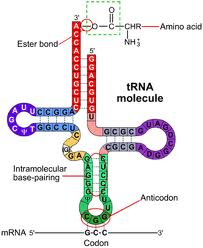
\includegraphics[width=2.2209in,height=2.0000in]{image/rnat1.jpg}
	\caption{Modelo de la estructura de una molécula de $_t$RNA [13].}	
	\label{ARNt}
\end{figure}		

La síntesis de proteínas se conoce también como \textbf{traducción}, dado que es la transferencia de información del lenguaje de los nucleótidos al de los aminoácidos. Este proceso ocurre en tres etapas: iniciación, elongación y terminación. Las mismas se dejan a criterio del lector.

\subsubsection{Excepciones al Dogma} 

\par Como se puede observar en la figura~\ref{excepcionesDogma}, existen dos excepciones al dogma conocidas como \textit{transcriptasa inversa o transcripción inversa} y \textit{replicación del RNA}.
\par La transcripción inversa\cite{curtis} es el proceso que consiste en la transferencia de información desde el RNA a la molécula de DNA y tiene lugar en los retrovirus\footnote{Un retrovirus es un virus RNA que se duplica en una célula huésped utilizando la transcriptasa inversa.}.
\par La replicación de RNA\cite{curtis} es el proceso que consiste en sintetizar RNA a partir de RNA y tiene lugar en algunos virus con genoma RNA (ejemplo TMV).
\par Los mecanismos mencionados escapan a este trabajo, por lo cual se deja a criterio del lector profundizar en éstos conceptos.
\begin{figure} [h]
	\hspace*{2cm}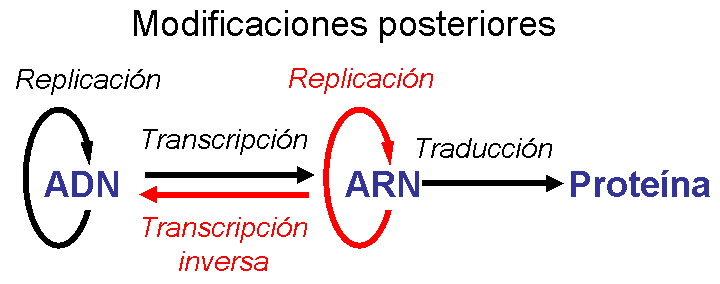
\includegraphics[width=3.8209in,height=0.9000in]{image/excepcionesDogma.jpg}
	\caption{Excepciones al Dogma Central [14].}
	\label{excepcionesDogma}
\end{figure}	

\vskip 1cm
\section{Estructura Secundaria del RNA} 
La estructura de una molécula de RNA se divide en tres niveles fundamentales de organización: primario, secundario y terciario. En particular, en este trabajo nos interesa el nivel secundario, por lo cual a continuación se abordará dicho nivel.

\par En términos generales, el plegamiento de una secuencia de RNA entre sus bases complementarias determina lo que se denomina \emph{Estructura Secundaria de RNA}. Conocer la estructura secundaria es fundamental para comprender el funcionamiento de los distintos tipos de RNA y de la célula en general. 

\par Más formalmente, dada una estructura primaria o secuencia de RNA de longitud $n$, la estructura secundaria es un conjunto S de pares $(i,j)$ con $1\leq i < j \leq n$ tal que para todo, $(i,j), (i',j') \in S$ se satisfacen las tres siguientes     condiciones:
\begin{itemize}
	\item $j-i > 3$
    \item $i=i' \Leftrightarrow j=j'$
    \item $i< i'\Rightarrow i < i' < j' < j \lor i < j < i' < j'$ 
\end{itemize}

\subsection{Predicción de la Estructura Secundaria (\textbf{\emph{folding}})}

\par El \emph{folding} o predicción de la estructura secundaria corresponde a un conjunto de técnicas bioinformáticas cuyo objetivo es predecir la estructura secundaria de una secuencia de RNA o de una proteína, basándose sólo en el conocimiento de su estructura primaria (secuencia de nucleótidos o de aminoácidos, respectivamente). Se da el caso en que diferentes secuencias de RNA pueden tener la misma estructura secundaria, por lo que también interesa determinar para una estructura secundaria dada, las secuencias de RNA que conservan esa estructura.

\par La existencia de una asociación entre la secuencia de aminoácidos y secuencia de nucleótidos respecto de la estructura secundaria adoptada en la proteína y el RNA respectivamente es la hipótesis fundamental sobre la cual están basados todos los métodos de predicción de estructura secundaria. 
 
\par En inglés, se suele denominar a la predicción de estructuras secundarias como \emph{folding} e \emph{inverse folding} al reconocimiento de posibles secuencias que conservan una estructura secundaria determinada. \emph{Inverse folding} escapa a este trabajo, pero puede obtenerse mayor información consultando el proyecto \textbf{vac-o}\footnote{\url{vac-o.googecode.com}}.

\par Esencialmente existen 2 tipos de algoritmos para determinar o predecir la estructura secundaria de una secuencia de RNA.
\begin{itemize} 
	\item \textbf{Predicción por mfe (Minimal Free Energy)}: propuesto e implementado por Michael Zuker en 1981\cite{Zuker81}, utiliza programación dinámica para encontrar la estructura secundaria que minimiza la energía libre.

	\item \textbf{Predicción comparativa}: utiliza diferentes métodos para comparar secuencias y estructuras con el fin de obtener una estructura por \\
	 ``consenso''\cite{Gardner04}.
\end{itemize}

Si bien la ``predicción comparativa'' presenta un incremento en la fidelidad de los resultados obtenidos con respecto a la ``predicción por mfe'', este tipo de algoritmos requieren la existencia de un conjunto de secuencias relacionadas entre sí (homólogas) y no siempre es posible obtenerlas. En particular, para este trabajo interesa poder conocer la estructura secundaria de una sola secuencia, por lo que la ``predicción comparativa'' fue descartada.

\par Entre las implementaciones de la ``predicción por mfe'' se destacan \textbf{UNAFold}\cite{unafold} y \textbf{RNAfold}\cite{Hofacker94}. Ambas implementan el algoritmo propuesto por Michael Zuker con complejidad $\mathcal{O}(N^{3})$ donde $N$ es la longitud de la secuencia. En el capítulo~\ref{analisis} se detallarán brevemente las implementaciones mencionadas.

\subsection{RNA Motifs}
\label{RNAmotifs}
El término ``Motifs''\cite{motifs}, también conocido como \emph{elementos regulatorios o sitios de unión} representa los diversos bloques que conforman una estructura secundaria de RNA. Juegan un papel funcional en la formación de la estructura terciaria y pueden estar sujetos a restricciones evolutivas. Dentro de estos bloques se encuentran:

\begin{itemize}

\item \emph{Single strand}: corresponde a un nucleótido no apareado (figura~\ref{motifs}.a).

\item \emph{Helices-Dúplex}: más de la mitad de los nucleótidos están presentes en las \emph{hélices} de doble cadena. Las regiones \emph{dúplex} pueden formar largas interacciones, las cuales son cruciales para determinar y estabilizar el pliegue global de una molécula de RNA. Los dúplex de RNA no son uniformes, aunque su variabilidad es menor que en el DNA. Estas variaciones dependen de la secuencia y el contexto estructural de la hélice con respecto al contexto global de la estructura tridimensional. (figuras~\ref{motifs}.b y~\ref{motifs}.c).

\item \emph{Bulges:} se forman cuando un tracto de la doble hélice se separa por uno o más nucleótidos no apareados. (figuras~\ref{motifs}.d y~\ref{motifs}.e).

\item \emph{Hairpins}: corresponde al elemento más común de una estructura secundaria y varían de 2 a 14 nucleótidos. Se forma cuando las secuencias nucleótidos de una misma cadena son estructuras complementarias invertidas.
Un \emph{hairpin} consiste de una región de bases apareadas (\emph{tallo}) y, a veces, incluye bases ``no apareadas'' intermedias (\emph{bucle}). Cuando las estructuras complementarias son contiguas, el hairpin presenta un tallo pero no un bucle. Los pequeño hairpin loop contienen un alto grado de estructura, mientras que los más largos (aquellos que contienen más de 7 u 8 nucleótidos no apareados) generalmente no están bien estructurados y termodinámicamente son menos estables. (figura~\ref{motifs}.f)
    
\item \emph{Internal Loop}: se forman cuando los dos tractos de la doble hélice se separan por uno o más nucleótidos no apareados. Los \emph{internal loop} puede ser simétricos o asimétricos, dependiendo del número de bases que contenga cada cadena. (figuras~\ref{motifs}.g y~\ref{motifs}.h y~\ref{motifs}.i)

\item \emph{Multi-Loop}: se forma por la intersección de dos o más dobles hélices. Estas dobles hélices se separan por secuencias de cero o más nucleótidos no apareados. (figura~\ref{motifs}.j)

\item \emph{External Loop}: motif inicial de una estructura (figura~\ref{motifs}.k) 

\end{itemize}
\par Las moléculas de RNA pueden contener numerosos motifs, lo que les permite plegarse y formar estructuras muy complejas tal como se puede observar en la figura~\ref{compleja}.

\vskip 10cm
\begin{figure} [!h]
	\begin{center}
		\vskip 2cm
		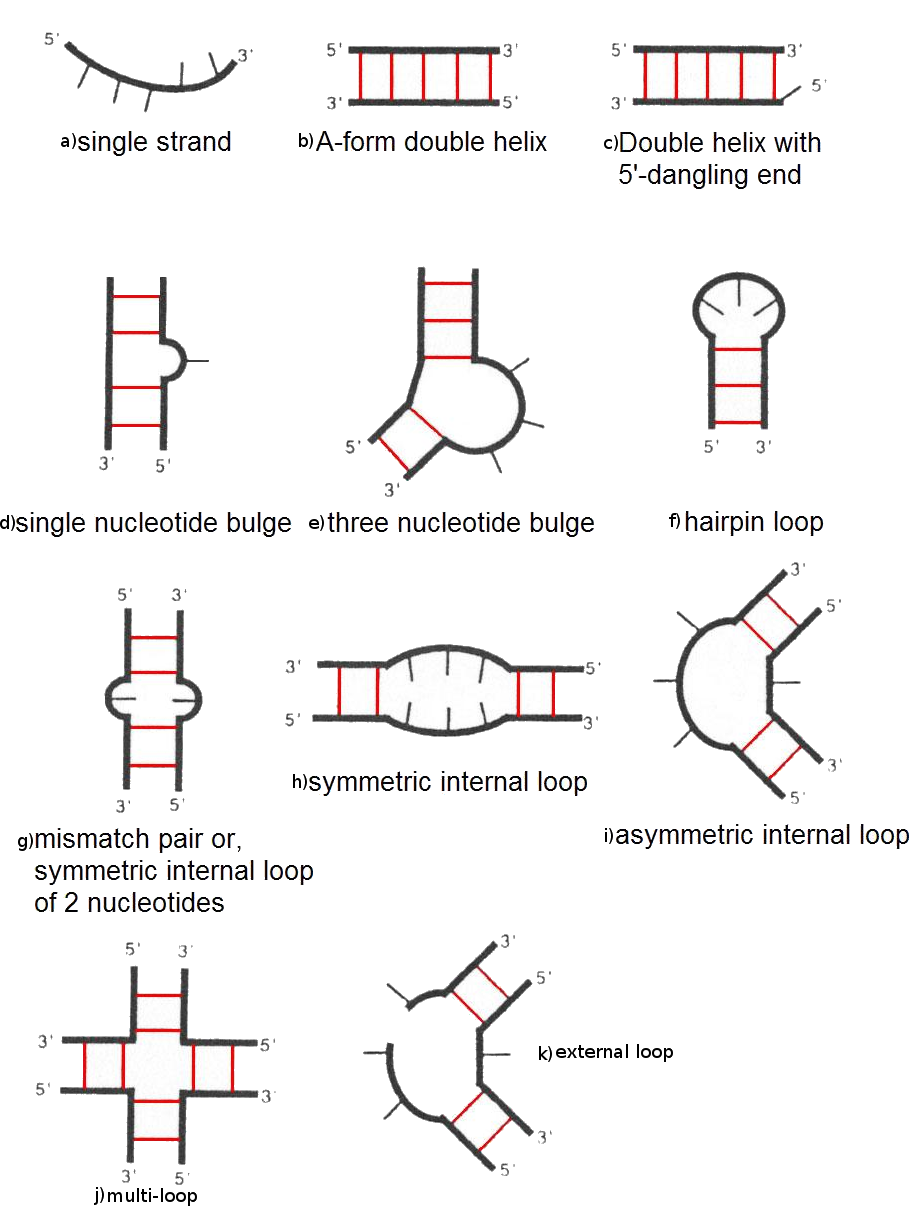
\includegraphics[width=5.5209in,height=5.3000in]{image/motifs2.png}
		\caption{RNA Motifs [2].}
		\label{motifs}
	\end{center}
\end{figure}

\begin{figure} [h]	
		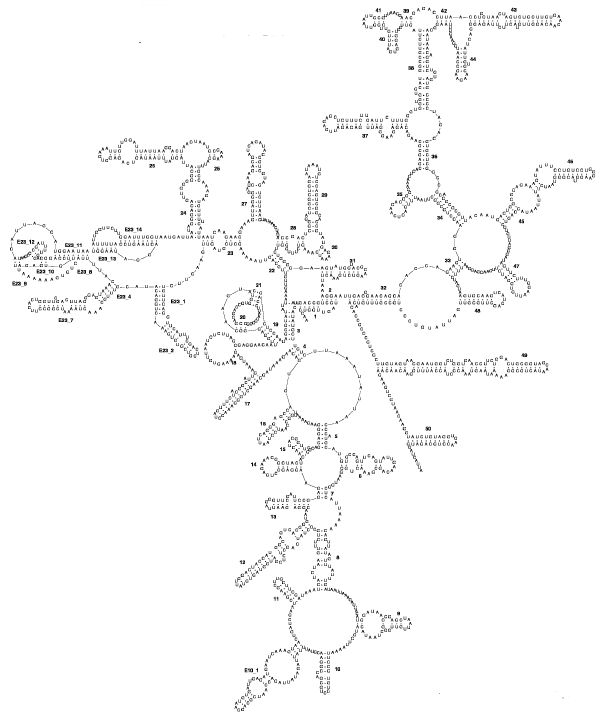
\includegraphics[width=5.8209in,height=5.2000in]{image/compleja.png}
		\caption{Estructura Secundaria Compleja [15].}		
		\label{compleja}	
\end{figure}	


\vskip 15cm
\section{Hibridación}
\par El fenómeno de apareamiento de bases (bases complementarias: A-T y C-G) para formar una doble hélice se llama \emph{hibridación}, dado que puede utilizarse para formar DNA híbrido compuesto por cadenas de diferentes orígenes tal como se exhibe en la figura ~\ref{hibridacion}.

\par Este proceso ocurre en solución y requiere de ciertos factores, tales como, un determinado pH, determinada temperatura, cierta concentración de sales, etcétera. Dependiendo de estas condiciones, es posible que en los híbridos existan malos apareamientos (A-C, por ejemplo).

\par El origen de cada una de las hebras es irrelevante, sólo importa la secuencia (que un número significativo de bases sea complementario entre las dos).

\begin{figure}[h!]
	\centering
		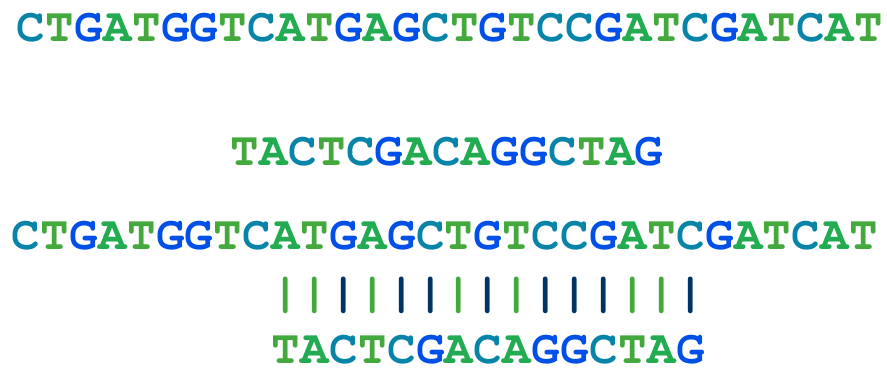
\includegraphics[scale=0.27]{image/hibridacion.png}
	\caption{Hibridación [2].}
	\label{hibridacion} 
\end{figure} 

\section{Energía Libre y Estabilidad} 
\par El concepto de ``Energía Libre'' hace referencia al total de energía contenida en un sistema que está disponible para realizar trabajo, como por ejemplo una molécula de RNA con una estructura secundaria, la cual le permite al mismo realizar trabajo. Una molécula de RNA puede estar dotada de una cierta cantidad de energía libre mediante interacciones eléctricas no neutralizadas en su estructura primaria, por lo tanto, esta energía se utilizará para plegar la misma hacia una estructura secundaria más estable. De este modo, un RNA con una estructura secundaria estable, implica una molécula en la cual sus interacciones eléctricas entre nucleótidos se hallan completamente neutralizadas. 
\par Este concepto es muy complejo e involucra nociones básicas de termodinámica, por lo cual su abordaje escapa al presente trabajo de ciencias de la computación, por lo cual puede indagarse más al respecto en \cite{energialibre}. 

\par La termodinámica de las interacciones RNA-RNA \\
\cite{freeEnergy} puede ser entendida como la suma de dos contribuciones de energía:
\begin{center}
	$\Delta$G = $\Delta$G$_u$ + $\Delta$G$_h$ 
\end{center}
donde:
\begin{itemize}
	\item $\Delta$G: energía libre.
	\item $\Delta$G$_u$: energía necesaria para exponer el sitio de unión para una interacción. 
	\item $\Delta$G$_h$: energía obtenida a partir de hibridación en el sitio de unión.
\end{itemize}

% \section{Relacionando conceptos}
% En la figura ~\ref{conceptos} se relaciónan las estructuras básicas mencionadas anteriormente.

% \begin{figure} 
%     \begin{center}
%         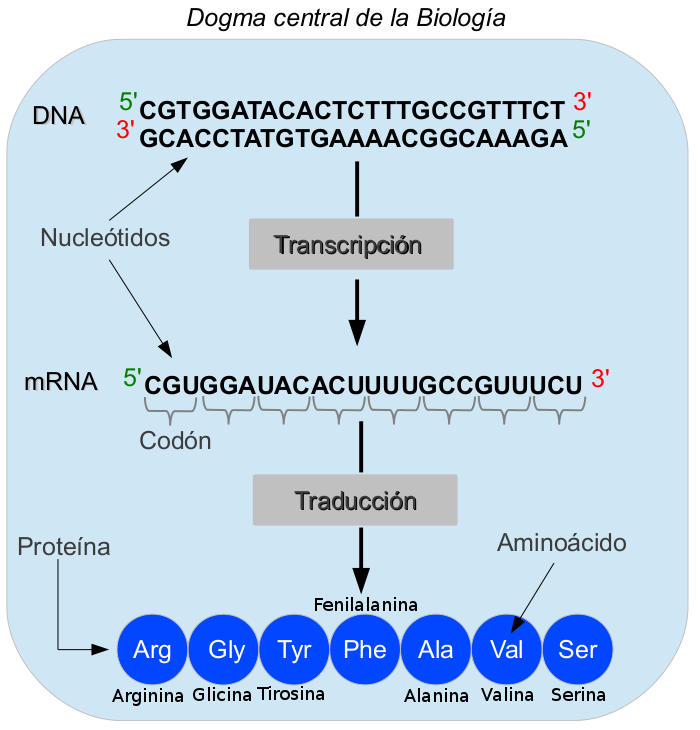
\includegraphics[width=5.209in,height=5.8000in]{image/resumen.png}
%     	\caption{Relacionando conceptos [3].}			
%     	\label{conceptos}
%     \end{center}
% \end{figure}
   
   
%II Remo
\part{Remo}
   \chapter{Descripción del Problema}

\epigraph{Rem tene, verba sequentur (Si dominas
el tema, las palabras vendrán solas).}%
{\textbf{Catón el Viejo}}

\par Se dice que todo problema nace a raíz de una dificultad, ésta se origina a partir de una necesidad en la cual aparecen dificultades sin resolver. De ahí, la necesidad de hacer un planteamiento adecuado del problema a fin de no producir efectos secundarios del problema con la realidad que se investiga. Por tanto, el planteamiento y descripción establece la dirección del estudio para lograr ciertos objetivos.

\section{Descripción General del Problema}

\par Para comprender la importancia y la hipótesis del presente trabajo se deben tener en cuenta diversos hechos referidos al código genético y los microRNA.

\par El código genético es un código organizado en \emph{tripletes} o \emph{codones}, donde tres nucleótidos codifican cada aminoácido de una proteína.
Si los codones constaran de una sola base, sólo habría capacidad para especificar cuatro aminoácidos ya que sólo hay cuatro bases diferentes en el DNA (C, G, A y T). Un código de dobletes podría tener 4x4 = 16 palabras de dos bases, o codones, lo cual es insuficiente para especificar sin ambigüedades veinte aminoácidos distintos. Por lo que, un código de tripletes da lugar a 4x4x4 = 64 codones, lo cual es más que suficiente para especificar los veinte aminoácidos\cite{genetica}. Tres de estos 64 codones son codones de terminación, que especifican la finalización de la traducción. Así, 61 codones llamados codones codificantes codifican los aminoácidos. Dado que hay 61 codones codificantes y sólo 20 aminoácidos distintos, el código contiene más información que la necesaria para especificar los aminoácidos, y se dice que es un \emph{código degenerado}, lo que implica que al menos uno de los tres nucleótidos (en general el último) puede ser distinto y sin embargo codificar para el mismo aminoácido\cite{genetica2}. Por otro lado, los codones que especifican un mismo aminoácido se consideran \emph{codones sinónimos}. Durante muchos años se supuso que el código genético era universal, lo que significa que cada codón especifica el mismo aminoácido en todos los organismos. En la actualidad se conoce que el código genético es casi, pero no completamente universal. En cada especie, se ha seleccionado una proporción de uso de codones que guarda relación con la proporción de RNA de transferencia correspondiente de manera de optimizar la síntesis proteica. Para otros patógenos intracelulares como los virus, existe una divergencia entre el uso de codones sinónimos\cite{holme} utilizado por el virus y el huésped correspondiente. El origen de esa divergencia no esta suficientemente claro.

\par Por otro lado, además de la molécula clásica de RNA (una sola hebra), existen diversos RNA pequeños, dentro de los cuales se destacan el RNA interferente pequeño ($_s$$_i$RNA) y el microRNA ($_m$$_i$RNA). Los $_s$$_i$RNA se dejan a criterio del lector su investigación ya que excede el presente trabajo.
Un $_m$$_i$RNA \cite{miRNA}\cite{miRNA2} es un RNA monocatenario, de una longitud de entre 21 y 25 nucleótidos, que tiene la capacidad de regular la expresión de otros genes mediante diversos procesos e inhibe la traducción del $_m$RNA. Los $_m$$_i$RNA se encuentran codificados en el genoma y juegan un papel importante en la regulación de la expresión proteica, procesos cancerosos e infecciones virales. 

\par Actualmente no hay evidencia respecto a si existe diferencia en cuanto a reconocimiento de $_m$$_i$RNA en los $_m$RNA originales de un virus y los $_m$RNA humanizados u optimizados (entendiéndose por este último término, la cadena de $_m$RNA del virus en la cual el uso de codones depende de la proporción del huésped). Para tal fin, es necesario determinar la capacidad de hibridación\footnote{Proceso por el cual se combinan dos cadenas de ácidos nucleicos antiparalelas con secuencias de bases complementarias en una única molécula de doble cadena, que toma la estructura de doble hélice, donde las bases nitrogenadas quedan ocultas en el interior.} de los $_m$$_i$RNA en la secuencia viral tal como existe en la naturaleza y en la secuencia humanizada, para poder establecer conclusiones al respecto. En otras palabras, determinar si el uso de codones divergente con respecto al huésped podría ser una consecuencia de la presión evolutiva generada por los $_m$$_i$RNA. Si esto es así, los $_m$$_i$RNA deberían tener menor capacidad de unirse al RNA viral que al genoma viral humanizado. 

\par En principio esta respuesta es importante desde el punto de vista biológico, y daría una herramienta importante para desarrollos posteriores, por ejemplo actualmente se está estudiando el uso de virus modificados para combatir cánceres, el programa podría predecir qué virus sería menos afectado por los $_m$$_i$RNA en células cancerosas y tenerlo en cuenta en el diseño del virus modificados.

\par Básicamente, el sistema a desarrollar comprenderá las siguientes característica:
\begin{itemize}
	\item Abarcar en su totalidad los requerimientos del problema.
	\item Construir un sistema que puede ser extendido en otros proyectos, brindando un diseño flexible. 
	\item Que proponga un buen uso de las prácticas de diseño para su mejor desempeño.
	\item Que posea documentación clara y precisa.
	\item Lograr un código fuente bien escrito y estructurado respetando las buenas prácticas de programación.
\end{itemize}

\section{Objetivos}
\par El principal objetivo de este trabajo es contrastar la teoría postulada y encomendada por el Dr. Roberto Daniel Rabinovich, la cual involucra principalmente la molécula de RNA como ya se puede inferir. 

\par En este trabajo se estudiará si la divergencia en el uso de codones sinónimos entre virus y huésped contribuye a disminuir la interferencia de los $_m$$_i$RNA en la expresión de los RNA mensajeros de origen viral. De esa manera se contribuirá a comprender mejor la relación virus-huésped y la evolución viral. Estos estudios tienen también una importancia potencial en la comprensión de la patogenia viral y en el desarrollo de herramientas terapéuticas como la terapia génica.

\par Para poder llevar a cabo el objetivo planteado anteriormente, será necesario elaborar una herramienta de software que realice entre otras cosas, múltiples comparaciones masivas de secuencias de $_m$$_i$RNA y $_m$RNA. Estas comparaciones pueden llevar un tiempo de cómputo demasiado alto, puesto que el número de combinaciones que surgen del cruce entre $_m$$_i$RNA y $_m$RNA puede ser un número lo suficientemente grande, esto se debe a que el tamaño de las secuencias de $_m$RNA pueden ser muy grandes. Además será necesario realizar pruebas en masa para poder obtener resultados confiables.
   \chapter{Metodología de Trabajo}

\epigraph{Nada se edifica sobre la piedra, todo
sobre la arena, pero nuestro deber es edificar
como si fuera piedra la arena.
}%
{\textbf{Jorge Luis Borges:} \\ \emph{Fragmentos de un evangelio apócrifo}}

\par Los sistemas de software requieren un tiempo y esfuerzo considerable para su desarrollo. Durante este tiempo, desde que se detecta la necesidad de construir un sistema de software, se identifican diferentes etapas que en conjunto se denominan \emph{el ciclo de vida del software}. En cada caso, en función de las características del proyecto, se configurará el ciclo de vida de forma diferente.
\par En particular, \remo se abordó empleando un enfoque metodológico que ordena rigurosamente las diversas etapas de desarrollo denominado \emph{Modelo de Desarrollo en Cascada}. A continuación se detallan algunos aspectos esenciales de dicho modelo y algunas consideraciones. 

\section{Modelo en Cascada}
\par El \emph{Modelo en Cascada Clásico} es un enfoque metodológico secuencial de desarrollo en el que los pasos de desarrollo son vistos hacia abajo (como una ``cascada de agua''), de tal forma que el inicio de cada etapa debe esperar a la finalización de la etapa anterior. La primera descripción formal de este método  fue desarrollada por Winston Royce W. (1929–1995) en 1970, aunque Royce no utiliza el término ``cascada'' en su artículo\cite{royce}. 

\subsection{Etapas del Modelo}
\label{modelo}
A continuación se detallan las diferentes etapas del modelo empleado.

\subsubsection{Elicitación de Requerimientos} 
\par Corresponde al estableciendo de los requisitos de todos los elementos que formarán parte del producto. En esta fase se analizan las necesidades de los usuarios finales del software para determinar qué objetivos debe cubrir. De esta fase surge un documento llamado \textit{``SRS''} (Documento de Especificación de Requisitos), que contiene la especificación completa de lo que debe hacer el sistema sin entrar en detalles internos.

\subsubsection{Análisis de Requerimientos}
\par Consiste en la investigación respecto al dominio de trabajo con el fin de comprender los requisitos de la etapa anterior. Se espera un conjunto de bibliografía y trabajos relacionados, con una breve descripción detallada de ellos (que se utilizará durante el diseño). 	
	
\subsubsection{Diseño}
\par El diseño del software se enfoca en cuatro atributos distintos del programa: la estructura de los datos, la arquitectura del software, el detalle procedimental y la caracterización de la interfaz. El proceso de diseño traduce los requisitos en una representación del software con la calidad requerida antes de que comience la codificación.
\par Como resultado de esta etapa surge el \textit{``SDD''} (Documento de Diseño del Software), que contiene la descripción de la estructura relacional global del sistema y la especificación de lo que debe hacer cada una de sus partes, así como la manera en que se combinan unas con otras.
\par Es conveniente distinguir entre diseño de alto nivel o arquitectónico y diseño detallado o de bajo nivel.

\subsubsection{Codificación}
\par Es la fase en donde se implementa el código fuente, haciendo uso de prototipos así como de pruebas y ensayos para corregir errores.

\subsubsection{Prueba}
\par La prueba se centra en la lógica interna del software, y en las funciones externas, realizando pruebas que aseguren que la entrada definida produce los resultados que realmente se requieren.

\subsection{Ventajas y Desventajas}
\par Luego de estudiar el modelo, se pueden detallar algunas ventajas y desventajas del mismo.
\begin{itemize}
    \item \textbf{Ventajas} 
	    \begin{itemize}    	
	    	\item La planificación es sencilla.
	    	\item Se tiene todo organizado y no se mezclan las fases.
	    	\item Las fases son conocidas por los desarrolladores ya que sigue los pasos intuitivos necesarios a la hora de desarrollar el software.
	    	\item Las etapas y actividades estan bien marcadas para facilitar la comprensión y claridad de los objetivos del proyecto.
	    \end{itemize}
	  
	\item \textbf{Desventajas}
		\begin{itemize}
			\item Iteraciones costosas.
			\item El cliente debe tener paciencia. Hasta llegar a las etapas finales del proyecto, no estará disponible una versión operativa del programa. 
			\item Un error importante no detectado hasta que el
            programa este funcionando puede ser desastroso. 
		\end{itemize}
\end{itemize}

\subsection{Consideraciones del Modelo}
\par Para implementar el presente modelo en cascada se tuvieron en cuenta ciertas consideraciones con respecto al contexto en que se desarrollo.

\par Por un lado, las etapas mencionadas en la subsección 3.1.1 fueron llevadas a cabo por una misma persona. En este sentido, se uso el \emph{modelo en cascada con ``solapamiento''}, también conocido como \emph{Sashimo}\cite{Mcconnell96}, que permite comenzar una etapa sin haber terminado por completo la etapa anterior. 

\par Por otro lado, el rol de ``cliente'' en el proceso de desarrollo fue llevado a cabo por miembros de \textbf{FuDePAN} que garantizaron el conocimiento del dominio del problema, no sólo permitiendo realizar la ``Especificación de Requerimientos'' sino que también contaban con los conocimientos técnicos de diseño y programación orientada a objetos como para supervisar el desarrollo. En este sentido, se tomaron algunos elementos de la variante al modelo de cascada “puro” que se conoce como \emph{Staged Delivery}\cite{Mcconnell96} o ``Implementación Incremental'', que permitió realizar revisiones periódicas con miembros de \textbf{FuDePAN} durante las diversas etapas. En la figura~\ref{cascade} se exhibe la estructura clásica del modelo, y las variantes mencionadas.

\begin{figure} [h]
	\hspace*{1cm}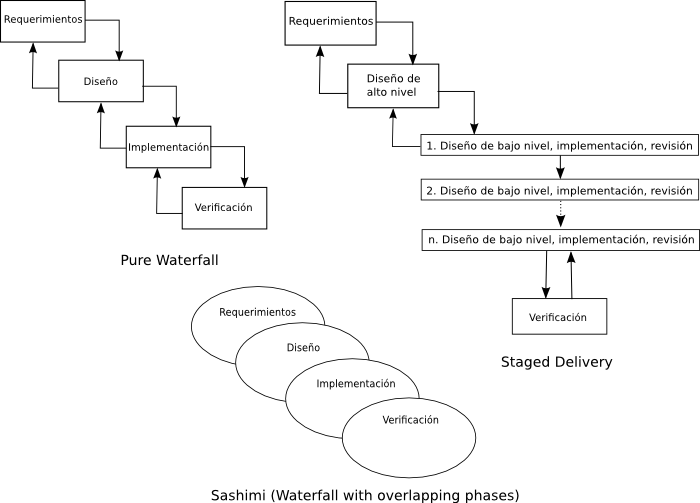
\includegraphics[width=5.2209in,height=3.300in]{image/modelOfCascade.png}
	\caption{Modelos en Cascada [17].}	
	\label{cascade}
\end{figure}

\section{Gestión de la Configuración}
\par Para desarrollar este proyecto fue necesario utilizar un manejador de versiones. Para ello se manipuló un repositorio \emph{Mercurial} (Hg) alojado en GoogleCode\footnote{\url{https://code.google.com/intl/es/}} con el fin de poder seguir la pista a todos los archivos que componen el proyecto.

\section{Prácticas de Software}
\par \remo se desarrolló empleando buenas prácticas de programación las cuales proporcionan múltiples ventajas al desarrollo. Éstas prácticas permiten mantener código limpio, de fácil lectura (sinónimo de fácil mantenimiento), reutilización e integración homogénea, entre otros factores.
A continuación se describen algunos aspectos orientados a \remo:

\begin{itemize}
    \item \textbf{Elicitación y análisis:} aproximadamente el 30 por ciento del tiempo total fue dedicado a éstas etapas, dado que fue necesario investigar el dominio del problema y diversas herramientas a emplear.     

    \item \textbf{Diseño:} se intentó obtener un diseño que respete, entre otras cosas, dos principios básicos: Simplicidad y Ocultamiento de la información. Se utilizaron Patrones de Diseño\cite{Gamma} y UML \\ \cite{uml}.

    \item \textbf{Construcción de código:} aproximadamente el 30 por ciento del tiempo fue dedicado a la construcción del código. Cada vez que se implementó un nuevo componente se chequeó la integración del mismo con todo el proyecto. Cuando superaba la prueba, el código fue transladado a la rama \emph{default} del repositorio.

    \item \textbf{Revisiones:} la mayoría de las operaciones \emph{commits} realizadas (incluyendo fuente, diagramas, documentos de responsabilidades, entre otros) fueron revisadas por al menos dos personas. No sólo se resaltaron errores, sino también cuestiones en cuando a calidad y eficiencia. Cada vez que se encontró un error o sugerencia, una nueva revisión fue creada conteniendo la solución.

    \item \textbf{Seguimiento de issues:} los bugs y defectos del proyecto fueron reportados como \emph{issues}. Luego, por cada issue, se creo una nueva revisión (rama) conteniendo la solución.
\end{itemize}

\section{Herramientas de Desarrollo Empleadas}
\par Tanto el sistema operativo como todas las herramientas que se usaron para el desarrollo del presente proyecto son libres. \remo tiene la licencia libre \textbf{GPL} (General Public Licence), una copia de la misma pude ser encontrada en \url{http://www.gnu.org/licenses/gpl-3.0.txt}.

\subsection{Lenguaje de Implementación}
\par Como lenguaje de implementación se utilizó \emph{C++}\cite{cplusplus}. 
\par \textit{C++}  es un lenguaje de programación diseñado en el año 1979 por \emph{Bjarne Stroustrup}\footnote{Científico de la computación y catedrático de Ciencias de la Computación en la Universidad A\&M de Texas.} en los laboratorios Bell\footnote{Centros de investigación científica y tecnológica ubicados en más de diez países y que pertenecen a la empresa estadounidense Lucent Technologies.}. En un principio fue una extensión del conocido lenguaje de programación C que fue denominado \emph{``C con clases''}. 

\par El nombre C++ fue propuesto por Rick Mascitti en el año 1983, cuando el lenguaje fue utilizado por primera vez fuera de un laboratorio científico. 

\par En la actualidad, es un lenguaje de tipado estático, multiparadigma, versátil, potente y de propósito general. Su éxito entre los programadores profesionales le ha llevado a ocupar el primer puesto como herramienta de desarrollo de aplicaciones. C++ mantiene las ventajas de C en cuanto a riqueza de operadores y expresiones, flexibilidad, concisión y eficiencia. Además, ha eliminado algunas de las dificultades y limitaciones del C original.

\par Este lenguaje fue elegido porque permite el uso de técnicas orientadas a objetos y produce eficiente código assembly. Además ofrece una gran cantidad de librerías para facilitar la resolución de determinados problemas, permitiendo concentrarse en los mismos y no en implementar tipos de datos abstractos ya conocidos.

\subsection{GNU}
\begin{itemize}
	\item \textbf{GCC (GNU Compiler Collection)\footnote{\url{http://gcc.gnu.org/}}:} conjunto de compiladores creados por el proyecto GNU.
     \textsc{GCC} es software libre y se distribuye bajo licencia \textsc{GPL}. Estos compiladores se
     consideran estándar para sistemas operativos derivados de GNU.

	\item \textbf{GDB (The GNU Project Debbuger)\footnote{\url{www.gnu.org/software/gdb/}}}: es un depurador portable que se puede utilizar en varias plataformas Unix y funciona para varios lenguajes de programación como C y C++ entre otros. \textsc{GDB} fue escrito por Richard 
    Stallman\footnote{Nacido en Manhattan, Nueva York, 16 de marzo de 1953. Fundador del movimiento por el software libre en el mundo.} en 1988, es software libre y se distribuye bajo licencia GPL. 
\end{itemize}	
	
\subsection{Sistema de Construcción}
Para la compilación e inclusión de librería externas, se usó \emph{fudepan-build}\footnote{\url{https://code.google.com/p/fudepan-build/}}, un proyecto de \textbf{FuDePAN} que utiliza scons\footnote{\url{http://www.scons.org/}}.

\subsection{\LaTeX}
\par Esta herramienta fue utilizada para llevar adelante el presente documento y todo la documentación de \textbf{Remo}. Básicamente \LaTeX{}\cite{latex} es un paquete de macros para TEX\footnote{Sistema de composición de textos de alta calidad creado por Donald E. Knuth a finales de la década de los 70, dirigido particularmente a aquellos textos que contienen una gran cantidad de expresiones matemáticas.}, originalmente escrito por Leslie Lamport para proporcionar un sistema de procesamiento de documentos más simple de uso que TEX, pero con toda su potencia. 
\par El formato de los archivos es mucho más estable que en otros procesadores de texto, cualquier cambio es realizado localmente y no repercute en efectos colaterales, existen implementaciones para distintas plataformas y en todas el resultado es exactamente el mismo (si se tienen los mismos estilos y tipos). 

\subsection{Edición}
\begin{itemize}
	\item \emph{Gedit\footnote{\url{http://projects.gnome.org/gedit/}}:} para la edición de texto plano.   
    \item \emph{Sublime\footnote{\url{www.sublimetext.com}}:} para la edición de texto plano. Permite simular un excelente IDE de desarrollo.
\end{itemize}

\subsection{Gráficos}
\begin{itemize}
	\item \emph{Gimp\footnote{\url{www.gimp.org}}:} editor de imágenes.
	\item \emph{Bouml\footnote{\url{http://www.bouml.fr/}}:} editor de diagramas UML.
	\item \emph{Dia\footnote{\url{http://live.gnome.org/Dia}}:} editor de diagramas de propósito general.
    \item \emph{Diagramas online\footnote{\url{www.websequencediagrams.com}}:} editor de diagramas de secuencia.
\end{itemize}

\subsection{Análisis Estático de Código}
\begin{itemize}
 \item \emph{Astyle}\footnote{\url{http://astyle.sourceforge.net}}: indentador de código fuente, formateador y embellecedor para los lenguajes C, C++, C\# y Java.

 \item \emph{cppcheck\footnote{\url{http://sourceforge.net/apps/mediawiki/cppcheck}}:} permite detectar los tipos de errores que los compiladores normalmente no detectan. El objetivo es detectar sólo los errores reales en el código (es decir, ningún falsos positivos).

\item \emph{Cloc\footnote{\url{http://cloc.sourceforge.net/}}:} es un programa para contar la cantidad de lineas del sistema.

\item \emph{CCCC\footnote{\url{http://cccc.sourceforge.net/}}:} herramienta que analiza los fuentes y genera reportes en varias métricas asociadas al código.

\item \emph{GCov\footnote{http://gcc.gnu.org/onlinedocs/gcc/Gcov.html}:} es una herramienta GNU para realizar pruebas de cobertura sobre código fuente. Se utiliza en conjunto con \textbf{\textit{gcc}} para determinar el número de veces que cada línea de un programa se ejecuta durante una ejecución. Esto hace que sea posible encontrar áreas del código que no se utilizan, o que no se ejecutan en los casos de pruebas  planteados.

\end{itemize}

\subsection{Análisis Dinámico de Código}
\begin{itemize}
	\item Valgrind\footnote{\url{http://valgrind.org}}: permite el análisis dinámico de código. Puede detectar automáticamente \emph{memory leaks} y errores de contexto.
\end{itemize}

\subsection{Automatización de Pruebas}
Se empleó gtest\footnote{\url{http://googletest.googlecode.com}} y gmock\footnote{\url{http://googlemock.googlecode.}} para la elaboración y ejecución de pruebas.
   \chapter{Elicitación y Análisis de Requerimientos}
\label{analisis}

\epigraph{No hay enigmas, si un problema puede plantearse, 
es que puede resolverse.}%
{\textbf{Ludwig Wittgenstein}}

\par El presente capítulo describe de forma general la elicitación de requerimientos, y de manera más detallada el análisis de los mismos.

\section{Elicitación de Requerimientos}
\par La IEEE\footnote{\url{www.ieee.org}} define los requerimientos como: 
\begin{center}
``Una condición de la capacidad que necesita un usuario para resolver un problema o lograr un objetivo. Una condición o una capacidad que debe cumplir un sistema para satisfacer un contrato, un estándar, una especificación, o cualquier otro documento oficial establecido.''
\end{center}
Los requerimientos de software del presente trabajo fueron provistos por miembros de \textbf{FuDePAN} y quedaron documentados en la ``Especificación de Requerimientos de Software'' (SRS) que se encuentra en el repositorio del proyecto. Dicho documento describe qué hará el software propuesto pero no cómo lo hará.

\subsection{Requerimientos Funcionales}
Los requerimientos funcionales de \remo pueden resumirse de la siguiente manera:

\begin{itemize}
	\item \textbf{Entrada:} dos archivos en formato FASTA (ver Apéndice~\ref{fasta}). El primero de ellos conteniendo un conjunto de secuencias de $_m$$_i$RNA, y el segundo, compuesto por múltiples secuencias de $_m$RNA.

	\item \textbf{Objetivo:} satisfaciendo las restricciones impuestas, determinar la relación de divergencia y contrastar la hipótesis plasmada anteriormente (luego de un extenso análisis biológico de los resultados). En este ámbito uno de los requisitos más importantes fue calcular la estructura secundaria de las secuencias de RNA (folding/hibridación).
							 
	\item \textbf{Salida:} archivos en formato CSV, que permitan poder establecer conclusiones al respecto. 
\end{itemize}

\par Uno de los principales requerimientos funcionales que cabe destacar tiene relación con la comparación de estructuras secundarias. Para ello, por cada RNA de entrada, es necesario calcular la estructura secundaria. A partir de la misma, realizar un reconocimiento de los diversos \emph{motif} (ver sección ~\ref{RNAmotifs}) que la componen para generar como salida un archivo comparativo. Las estructuras pueden ser muy grandes y complejas, tales como la que se exhibió en la figura~\ref{motifs}.

\par Desde el punto de vista del diseño, \remo debía cumplir con los principios de diseño conocido por el acrónico SOLID\footnote{Acrónimo nemotécnico introducido por Robert C. Martin en la década del 2000, que representa cinco principios básicos de la programación y diseño orientado a objetos}~\cite{Martin00}. Estos principios son los siguientes y se retomaran el la sección~\ref{disenio}:
\begin{itemize}
	\item \textbf{S}ingle responsibility principle (SRP)
	\item \textbf{O}pen/closed principle (OCP)
	\item \textbf{L}iskov substitution principle (LSP)
	\item \textbf{I}nterface segregation principle (ISP)
	\item \textbf{D}ependency inversion principle (DIP)	
	\item Law of Demeter (LoD)
\end{itemize}

\par Para observar detalladamente los requerimientos funcionales puede consultarse el SRS\footnote{\url{r-emo.googlecode.com}} correspondiente a \remo.

\section{Análisis de los Requerimientos}
\par El objetivo básico del análisis de problemas es obtener una comprensión clara de las necesidades de los clientes, en otros término, qué es exactamente lo que se desea del software, y cuales son las limitaciones de la solución. El principio elemental empleado en el análisis es el mismo que en cualquier tarea compleja: \emph{divide y vencerás}. Esto es la “partición” del problema en subproblemas y a continuación, tratar de entender cada subproblema y su relación con otros subproblemas en un esfuerzo por entender el problema total.

\par Una vez identificados los diversos requerimientos, se realizó un extenso análisis referente a las herramientas a emplear y al dominio del problema en general. A continuación se detalla dicho análisis.

\subsection{Búsqueda de datos mínimos}
	\par Esta etapa consistió en la recolección de datos necesarios para posteriormente realizar las primeras pruebas de \textbf{Remo}. Esta fase involucró la recolección de secuencias de $_m$RNA, secuencias de $_m$$_i$RNA y el software humanizador de secuencias. 
	
\subsubsection{$_m$RNA}
	\par La bases de datos biológicas son DNA céntricas, es decir que si un virus tiene su información como RNA, la secuencia archivada esta expresada como DNA (\textbf{T}imina en lugar de \textbf{U}racilo). Por lo cual, no se encontró $_m$RNA directamente, sino que como gen.

	\par Los virus obtenidos para las pruebas se obtuvieron de \\
	~\cite{holme}. Dicha publicación menciona el número de acceso a \emph{GenBank}\footnote{Base de datos de secuencias genéticas. Colección de todas las secuencias de DNA disponibles al público. La base de datos GenBank está diseñada para proporcionar y fomentar el acceso de la comunidad científica a la mayor parte de información actualizada y completa la secuencia de DNA. Por lo tanto, \textit{NCBI} (National Center for Biotechnology Information \url{http://www.ncbi.nlm.nih.gov/}) no impone restricciones sobre el uso o la distribución de los datos GenBank.} para su obtención. A continuación se exhiben algunos de los códigos que se mencionan el artículo: 
	\begin{itemize}
		\item Coxsackievirus A9 (Griggs; \textsc{D00627}).
		\item Enterovirus 71 (TW/2272/98; \textsc{AF119795}).
		\item Hepatitis A virus (HAF-203; \textsc{AF268396}).
		\item Poliovirus type 3 (23127; \textsc{X04468}).
		% \item Rhinovirus type 89 (HRV89; \textsc{M16248}).
		% \item Hepatitis E virus (Hyderabad; \textsc{AF076239}).
		% \item Norwalk virus (BS5; \textsc{AF093797}).
		% \item Astro-virus type 1 (Oxford; \textsc{L23513}).
		\item Dengue-1 virus (PDK-13; \textsc{AF180818}).
		% \item Dengue-2 virus (S1; \textsc{NC\_001474}).
		% \item Dengue-3 virus (H87; \textsc{M93130}).
		% \item Dengue-4 virus (\textsc{NC\_002640}).
		% \item GB virus C (G05BD; \textsc{AB003292}).
		% \item Hepatitis C virus (HCV-A; \textsc{AJ000009}).
		% \item Japanese encephalitis virus (GP78; \textsc{AF075723}).
		% \item Murray Valley virus (MVE-1-51; \textsc{AF161266}).
		% \item West Nile virus (2741; \textsc{AF206518}).
		% \item Western tick-borne encephalitis virus (Neudoerfl; \textsc{U27495}).
		\item Yellow fever virus (Trinidad 79A; \textsc{AF094612}).
		% \item Eastern equine encephalitis virus (\textsc{U01034}).
		% \item O’nyong-nyong virus (SG650; \textsc{AF079456}).
		% \item Ross River virus (NB5092; \textsc{M20162}).
		\item Rubella virus (Cendehill; \textsc{AF188704}).
		% \item Sindbis virus (Edsbyn 82-5; \textsc{M69205}).
	\end{itemize}

	\par A partir de los códigos de acceso, desde \url{http://www.ncbi.nlm.nih.gov/genbank/} se obtuvieron los DNA de cada virus en formato FASTA. Para traducir los DNA a RNA (reemplzado de \textsc{U} por \textsc{T}), se utilizó la herramienta \emph{BioEdit}\footnote{\url{http://www.mbio.ncsu.edu/BioEdit/bioedit.html}}. 

	% Alternativamente, se usó de la herramienta \emph{Jalview}\footnote{\url{http://www.jalview.org/}} y la librería \textit{Biopp}\footnote{\url{biopp.googlecode.com}}. 

\subsubsection{$_m$$_i$RNA}
	\par Se obtuvo una base de datos\footnote{Descargada de \url{http://www.mirbase.org/cgi-bin/mirna\_summary.pl?org=hsa}} de $_m$$_i$RNA en formato FASTA. De la misma, se seleccionaron al azar aproximadamente 50 $_m$$_i$RNA para luego realizar las primeras pruebas. Los $_m$$_i$RNA están formados por 22 nucleótidos aproximadamente. A continuación se exhiben algunas de las secuencias: 
\begin{itemize}
	\item \textsc{AAGAUGUGGAAAAAUUGGAAUC}
	\item \textsc{CAGUGGUUUUACCCUAUGGUAG}
	\item \textsc{CAGGCAGUGACUGUUCAGACGUC}
	\item \textsc{AUCAUAGAGGAAAAUCCAUGUU}
	\item \textsc{AAGAAGAGACUGAGUCAUCGAAU}
	\item \textsc{CUCUAGAGGGAAGCGCUUUCUG}
	\item \textsc{GUUUGCACGGGUGGGCCUUGUCU}
	\item \textsc{AAAGACCGUGACUACUUUUGCA}
	\item \textsc{UGUAAACAUCCCCGACUGGAAG}
\end{itemize}
		
	\par Otras bases de datos de $_m$$_i$RNA consultadas fueron: 
		\par \hspace*{1cm} • \url{http://micrornadatabase.com/}.
		\par \hspace*{1cm} • \url{http://microrna.org/}.
		\par \hspace*{1cm} • \url{http://mirdb.org/miRDB/}.
		\par \hspace*{1cm} • \url{http://www.mirbase.org/}.

\subsection{Herramientas y Librerías}
\subsubsection{GeneDesign}
\emph{GeneDesign}\footnote{Descarga de: \url{https://github.com/GeneDesign/GeneDesign}}~\cite{geneDesign} fue el software empleado para la ``humanización'' de las cadenas de nucleótidos. El mismo, corresponde a un software libre usado por biólogos moleculares, el gobierno y los sectores farmacéuticos, químicos, agrícolas y biotecnológicos para el diseño~\cite{Welch}, clonación y validación de secuencias genéticas.

\par \emph{GeneDesign} automatiza el proceso de determinar qué pares de bases deben ser unidos entre sí en un orden determinado para un gen. Un gen codifica para una proteína específica, y el orden de los cientos o miles de pares de bases que componen ese gen determina el orden de los bloques de construcción de aminoácidos que componen esa proteína.  

\par Este software, consta de seis módulos que pueden ser utilizados individualmente o en serie para automatizar las tareas necesarias para diseñar y manipular secuencias de DNA sintético. 

\par Se presentaron tres opciones para el uso de este software:
	\begin{itemize}
		\item \emph{Instalado:} corresponde a tener \emph{geneDesign} instalado en la PC, y el producto a desarrollar lo invocará a medida que lo requiera.
		\item \emph{Online:} el producto a desarrollar utiliza \emph{geneDesign} de forma online a medida que lo necesita. (\url{http://genedesign.thruhere.net/gd})
		\item \emph{Offline:} correr de forma online \emph{geneDesign} y generar con su salida dos archivos en formato FASTA. Uno de ellos, con el $_m$RNA original, y el otro con el humanizado. Luego el producto a desarrollar tomará los archivos mencionados como entrada.
	\end{itemize}
	
\par \remo empleó la opción número 1 (\emph{Instalado}) otorgando de esta forma mayor independencia y evitando la necesidad de conexión a internet para obtener los resultados. Para esta opción fue necesario descargar el código de \emph{geneDesign} del repositorio git e instalar y configurar el servidor web \emph{apache2}\footnote{url{http://httpd.apache.org/}}.

\par Cabe destacar que se encontró un bug en el código, básicamente el software siempre realizaba la conexión al servidor central por lo cual, aunque se ejecutara localmente con el servidor apache, no funcionaba sin conexión a internet, dado que siempre se establecía un socket con el servidor central.

\subsubsection{Librerías a Utilizar}
Además de las librería estándares que provee el jugoso lenguaje de programación C++, cabe mencionar las siguientes:
\begin{itemize}
	\item \emph{MiLi\footnote{\url{mili.googlecode.com}}}: es una colección de pequeñas y útiles librerías desarrolladas en el 
	lenguaje de programación C++ por \textbf{FuDePAN}, compuestas únicamente por cabeceras (\emph{headers}). No requiere
	instalación para su uso y ofrece \emph{soluciones simples para problemas sencillos}.
		 
	\par Dentro de las diversas funcionalidades podemos encontrar:
	\begin{itemize}
		\item \textbf{binary-streams:} permite serializar diferentes tipos de datos dentro de un único objeto utilizando los
		 operadores de stream ($\ll$ y $\gg$). Hay dos maneras de utilizar esta librería:
			\begin{enumerate}
				\item Empaquetar datos dentro de un objeto de salida (bostream) utilizando el operador $\ll$.	
				\item Extraer datos desde un objeto de entrada (bistream) utilizando el operador $\gg$.
			\end{enumerate}
		\item \textbf{container-utils:} esta biblioteca provee un conjunto de funciones, optimizadas para cada tipo de 					contenedor STL:
				\begin{itemize}
					\item \textsf{find(container, element)}.
					\item \textsf{find(container, element, nothrow)}.
					\item \textsf{contains(container, element)}.
					\item \textsf{insert into(container, element)}.
					\item \textsf{copy container(from, to)}.
				\end{itemize}
				\par Adicionalmente, esta biblioteca provee las siguientes clases:
				\begin{itemize}
					\item \textsf{ContainerAdapter$<$T$>$}.
					\item \textsf{ContainerAdapterImpl$<$T, ContainerType$>$}.
				\end{itemize}
				\par Estos container adapters son una herramienta para lidiar con diferentes contenedores \textsc{STL} de manera 					homogénea, sin necesidad de conocer el tipo de contenedor que es (vector, list, map, set). Los usuarios pueden 					invocar al método \textsc{insert (const T\&)} para insertar un elemento de tipo \textsc{T} sin la necesidad de 					saber el tipo del contenedor.

		\item \textbf{generic\_exception:} ofrece una implementación de excepciones genéricas a partir de las cuales los 			desarrolladores pueden crear sus propias excepciones para problemas específicos de una manera muy simple.
	\end{itemize}
		
	\item \emph{Biopp\footnote{\url{biopp.googlecode.com}}}: corresponde a una biblioteca C++ para Biología Molecular. La misma
	 provee las diversas estructuras de datos y métodos para manipular las secuencias de nucleótidos con las que se trabajó. 

	\item \emph{Biopp-filer\footnote{\url{biopp-filer.googlecode.com}}}: refiere a una librería de persistencia para 
	\emph{Biopp}. Esta librería se utilizó para leer las secuencias en formato FASTA.

	\item \emph{Getoptpp\footnote{\url{getoptpp.googlecode.com}}}: es una librería que proveerá entre otras cosas, diversas
	 funciones para el manejo de la entrada estándar.
\end{itemize}

\subsection{Librerías a Implementar}
\label{libreriaAImplementar}

\par Como resultado del análisis y pensando en la correcta modularización y futuros desarrollos, surgió la necesidad de implementar las siguientes librerías: 

\begin{itemize}
	\item \textbf{fideo (Folding Interface Dynamic Exchange Operations): } el problema que se presentó radica en que cada librería externa tanto para folding como para hibridación, poseen diferentes formas de recibir los parámetros de entrada y diferentes formas de retornar los resultados que generan. A razón de esto se decidió implementar \emph{fideo} como una forma de unificar el acceso a estas librerías externas e integrarlas al resto del sistema. Básicamente, se encargará de proveer las funcionalidades necesarias para obtener la energía libre de una secuencia de nucleótidos. Esta librería se utilizará para la invocación externa de los programas de cálculo de estructura secundaria (folding e hibridación). Por un lado, incluye los backends UNAFold y RNAFold para folding, y por el otro, incluye los backends RNAup, RNAcofold, RNAduplex, IntaRNA y RNAHybrid para la hibridación. Fideo provee la abstracción necesaria para poder utilizar indistintamente cualquiera de los backends mencionados de forma transparente.

	\item \textbf{acuoso (Abstract Codon Usage Optimization Software for Organisms): } permite la optimización (humanización) de secuencias. La idea es similar a fideo, dado que permite realizar este servicio con cualquier software de manera muy simple. Inicialmente se implementó empleando \emph{GeneDesign}, pero de manera sencilla puede agregarse cualquier otro backend.

	\item \textbf{etilico (External Tools Invocation LIbrary and COmponents)}: básicamente corresponde a una librería estática compuesta por diversas funciones necesarias y de uso común para invocación de librerías, manejo de archivos temporales y diversos componentes.
\end{itemize}

\subsection{Backends para Folding}

\subsubsection{UNAFold}
\label{unafold}
\par Inspirado en el famoso software ``mfold'', el paquete de software \emph{UNAFold}~\cite{unafold} es un conjunto integrado de programas (empleando programación dinámica~\cite{ProgDinaminca}) que simulan el folding, la hibridación y la vías de fusión para una o dos secuencias de cadena simple de ácido nucleico. El paquete predice el folding para RNA de cadena simple o el DNA a través de la combinación de minimización de la energía libre, los cálculos de función de partición y muestreo estocástico. El nombre se deriva de ``Folding Unificado de Ácido Nucleico''. Acepta tanto archivos planos (que contengan únicamente nucleótidos) como en formato FASTA. Está disponible para su descarga en \url{http://www.bioinfo.rpi.edu/applications/hybrid/download.php.}
A continuación se exhibe el cálculo de folding de una secuencia de prueba.

{\scriptsize
	\begin{verbatim}
        gringusi@gringusi:~$ echo "AAAAAAAAGGGGGGGGCCCCCCCCTTTTTTTT" > seq.fasta
        gringusi@gringusi:~$ UNAfold --max=1 seq.fasta

        Checking for boxplot_ng... not found
        Checking for hybrid-plot-ng... found, supports Postscript
        Checking for sir_graph_ng or sir_graph... not found
        Checking for ps2pdfwr... found
        Calculating for seq.fasta, t = 37
        gringusi@gringusi:~$ l
        seq.fasta seq.fasta_1.ct seq.fasta.ann seq.fasta.ct seq.fasta.det seq.fasta.dG 
        seq.fasta.h-num seq.fasta.plot seq.fasta.rnaml seq.fasta.run seq.fasta.ss-count
    \end{verbatim}
}

Dentro de los diferentes archivos generados se detacan el \emph{.dG}, \emph{.ct} y \emph{.det}. El primero de ellos contiene el valor de la energía libre en la unidad kcal/mol. El segundo,  define una secuencia de ácido nucleico, junto con su estructura secundaria. Puede contener pliegues múltiples de una secuencia única o incluso múltiples plegamientos. Por último, el tercero, brinda la estructura secundaria en un formato particular, donde se pueden identificar los diversos \emph{motifs} que la componen.

\subsubsection{RNAFold}
\label{rnafold}
\par Básicamente lee secuencias de RNA de entrada estándar y calcula el mínimo de energía libre (MFE), la función de partición (pf) y una matriz de probabilidad en base al apareamiento. Devuelve como salida la estructura mfe en notación soporte (empleando ``()''), su energía, la energía libre del conjunto termodinámico y la frecuencia de la estructura mfe. También produce archivos PostScript con parcelas de la gráfica resultante estructura secundaria y un ``gráfico de puntos'' de la matriz de apareamiento de bases. Para comprender mejor su comportamiento y método consultar~\cite{vienna}.

\par Está disponible para su descarga en \url{http://mfold.rna.albany.edu/?q=DINAMelt/software.}

{\scriptsize
	\begin{verbatim}
        gringusi@gringusi:~$ RNAfold

        Input string (upper or lower case); @ to quit
        ....,....1....,....2....,....3....,....4....,....5....,....6....,.
        AAAGGCAACGGCCAU
        length = 15
        AAAGGCAACGGCCAU
        ...(((....))).. 
        minimum free energy =  -4.40 kcal/mol
	\end{verbatim}
}

\par El resultado obtenido es, precisamente, la energía libre y la estructura secundaria representada con paréntesis y puntos, donde los pares de paréntesis indican las bases ``apareadas'' o ``unidas'' y los puntos, las bases libres.

\subsection{Backends para Hibridación} %mirar bien referencias
\label{hibrid}

\subsubsection{IntaRNA}
\par \emph{IntaRNA~\cite{intaRNA}} predice interacciones entre dos moléculas de RNA, por ejemplo, un RNA no codificante (e.g
ncRNA) y un mRNA. El scoring se basa en la energía combinada de interacción que resulta de la suma de la energía libre de hibridación y la energía libre necesaria para la fabricación de los sitios de interacción accesible de ambas moléculas.

\par La interacción tiene que contener la semilla de una interacción, es decir, una región (casi) perfecta de complementariedad para facilitar el inicio de la interacción. Las características de esta región de semilla son definidas por el usuario.

\par La accesibilidad se define como la energía libre necesaria para desplegar el sitio de interacción en cada molécula. Requiere del paquete de Vienna RNA (versiones 1.8.2/1.8.5). La versión 1.8.5 puede descargarse de \url{http://www.bioinf.uni-freiburg.de/Software/index.html?en\#IntaRNA-download}

\par Existen dos variantes para realizar la predicción, la primera corresponde una aproximación completa, que es O(n2 m2) en el tiempo y O(nm) en el espacio al restringir el tamaño de los bucles internos y donde n y m son las longitudes de las secuencias de RNA que interactúan (n $>$ m), y la segunda que es una simplificación heurística de la aproximación completa, que tiene una complejidad en tiempo de O(nm) y un espacio de complejidad O(nm), donde m = max {m, L 3} y L es el tamaño de la secuencia de la ventana en el que tanto el $_m$RNA diana y la sRNA se pliegan.

\subsubsection{RNAup}
\par \emph{RNAup~\cite{rnaup}} calcula la termodinámica de las interacciones RNA-RNA, por descomposición de las uniones a
través de dos etapas. La termodinámica de tales interacciones RNA-RNA puede ser entendida como la suma de dos contribuciones de energía: la energía necesaria para ``abrir'' el sitio de unión, y la energía obtenida de la hibridación.

\par En primer lugar se calcula la probabilidad de que un potencial sitio de unión siga siendo desapareado, lo que es equivalente a calcular la energía libre necesaria para romper las uniones. En segundo lugar, este cálculo se combina con la energía de interacción para obtener la energía total de unión.

\par Proporciona dos modos: por defecto calcula accesibilidad (en términos de energía libre para romper uniones, de longitud 4) y muestra la región de mayor accesibilidad y la energía libre necesaria para su apertura. En modo interacción, se calcula la interacción entre dos RNA. Este modo se activa si la entrada se compone de dos secuencias concatenadas por un ``\&'' o si se emplea el flag -X[pf] o -b.

\par  La energía libre ``dG'' se divide en sus componentes ``dGint'' (energía de interacción) y ``dGu\_l'' (energía de apertura).                      

\par \emph{RNAup} esta incluido en el paquete de Vienna RNA~\cite{vienna}}. La última versión corresponde a la 2.0.7 y esta disponible para su descarga en \url{http://www.tbi.univie.ac.at/~ivo/RNA/}.

\subsubsection{RNACofold}
\par \emph{RNACofold} funciona como \emph{RNAfold}, pero permite especificar dos secuencias de RNA que formará una estructura de dímero\footnote{Complejo macromolecular formado por dos macromoléculas, como proteínas y ácidos nucleicos, usualmente mediante enlaces no covalentes.}.             

\par Las secuencias de RNA se leen por entrada estándar, cada línea de entrada corresponde a una secuencia, a excepción de las líneas que comienzan con ``>'', que contiene el nombre de la siguiente secuencia. Para calcular la estructura híbrida de dos moléculas, las dos secuencias deben ser concatenadas usando el carácter ``\&'' como separador. 
            
\par Al igual que RNAup, \emph{RNAcofold} esta incluido en el paquete de Vienna RNA~\cite{vienna}. Tiene orden O($n^{3}$)
    
\subsubsection{RNADuplex}
\par Básicamente lee dos secuencias de RNA por entrada estándar o desde un archivo y calcula las estructuras secundarias óptimas y subóptimas para su hibridación. El cálculo se simplifica al permitir sólo pares de bases inter-moleculares (corresponde a un caso específico de \emph{RNAcofold}). 

\par La estructura calculada óptima y subóptima se retornan por salida estándar, una por línea. Cada una de ellas consiste en: la estructura de soporte en formato de punto con una ``y'' que separan las dos hebras, el rango de la estructura en las dos secuencias en el formato \emph{``from,to : from,to''}, la energía de estructura dúplex en kcal/mol.

\par El formato es especialmente útil para el cálculo de la estructura híbrida entre una secuencia pequeña y una secuencia larga. Al igual que los dos anteriores, \emph{RNAduplex} esta incluido en el paquete de Vienna RNA~\cite{vienna}.         

\subsubsection{RNAHybrid}
\par \emph{RNAHybrid~\cite{rnahybrid}} es una herramienta para encontrar hibridaciones de mínimo de energía libre entre una
secuencia larga (target) y un RNA corto (query). La hibridación se lleva a cabo de la siguiente manera: la secuencia corta se hibrida con las mejores partes de fijación del target.

\par \emph{RNAHybrid} puede obtenerse desde \url{http://bibiserv.techfak.uni-bielefeld.de/download/tools/rnahybrid.html}.  Actualmente, puede utilizarse como servicio web desde \url{http://alk.ibms.sinica.edu.tw/cgi-bin/RNAhybrid/RNAhybrid.cgi}.
Tiene orden O(nm).

   \chapter{Diseño}
\label{disenio}

\epigraph{La mejor estructura no garantizará los
resultados ni el rendimiento. Pero la
estructura equivocada es una garantía de
fracaso.}%
{\textbf{Peter Drucker}}

\par Según la IEEE el diseño es definido como: \emph{``El proceso de definición de la arquitectura, componentes, interfaces y otras características de un sistema o componente que resulta de este proceso''}[IEEE610.12-90]. Así, todo sistema necesita de un diseño adecuado que permita modelar adecuadamente los requerimientos con el objetivo de tener una mirada integradora del sistema. Un buen diseño ayuda a crear software con propiedades deseables, como reusabilidad, mantenibilidad, portabilidad, ente otras.

\par De manera similar a la elicitación de requerimientos, la descripción detallada del diseño se encuentra documentada en la “Especificación de Diseño de Software”. Análogamente a los capítulos anteriores, sólo se detallarán los aspectos más relevantes del diseño, dejando como lectura adicional el mencionado documento.
 
\section{Responsibility-Driven Design}
\par Este esquema fue empleado para el análisis y descripción del diseño de \textbf{Remo}. Fue propuesto inicialmente por Rebeca Wirfs-Brock y Brian  \\
Wilkerson\cite{ResponsibilityDesign} en 1990. Básicamente, se enfoca en qué responsabilidades deben ser cubiertas por el sistema y en cuáles serán los objetos responsables de llevarlas a cabo. 

\par Inicialmente, se describen las acciones y actividades que constituyen las ``responsabilidades'' del sistema. Luego, se describen dichas responsabilidades en un lenguaje comprensible, tanto para el usuario como para el desarrollador, y finalmente, se diseñan objetos de software que las implementen apropiadamente. En primera instancia, se captura la noción de cuál es el comportamiento deseado, antes de plantear la forma de obtener dicho comportamiento.

\section{Principios de Diseño}
\par Uno de los requerimientos de \remo fue que se respetara los principios del diseño orientado a objetos resumidos en el acrónimo SOLID\cite{Martin00} introducido por Robert C. Martin\footnote{Autor de varios libros tales como ``Object-orineted Design'' y ``Agile Development''.} a principios del año 2000.

\par En particular se puso especial atención en respetar los principios SRP, OCP y DIP debido a que repercuten directamente en que el sistema sea más simple de mantener y extender con nuevas funcionalidades. Además, el principio DIP es fundamental para lograr un software que sea verificable mediante la automatización de pruebas como se pudo comprobar más adelante, en la etapa de “verificación”.

A continuación se detalla brevemente cada uno de los principios, dado que resultan de gran importancia su conocimiento.

\begin{itemize}
	\item \textbf{Principio de Simple Responsabilidad (SRP):} establece que no debería haber nunca más de una sola razón para que una clase cambie. En el contexto de este principio, llamamos responsabilidad a una razón de cambio. Si una clase tiene más de una responsabilidad, las responsabilidades se acoplan. Esta clase de acoplamiento lleva a que el sistema no sea tolerante a las modificaciones. Básicamente, refiere a la noción de que un objeto debe tener sólo una responsabilidad.
	
	\item \textbf{Principio de Apertura-Cierre (OCP):} este principio afirma que las entidades de software (clases, módulos, funciones, etcétera) deben estar abiertas para la extensión, pero cerradas para la modificación. Esto es especialmente valioso en un entorno de producción, donde los cambios en el código fuente puede requerir revisiones de código, pruebas unitarias, y otros procedimientos para calificar para su uso en un producto.
	\par Este principio indica que cuando se cambian los requisitos, se extiende el comportamiento de los módulos mediante la adición de código, pero el código viejo no se cambia dado que funciona.

	\item \textbf{Principio de Sustitución de Liskov (LSP):} refiere a que los objetos de un programa pueden ser reemplazados por instancias de sus subtipos, sin alterar la exactitud del programa.
	\par Se afirma que, en un programa, si \textsc{S} es un subtipo de \textsc{T} (\textsc{T}$\to$\textsc{S}), entonces los objetos de tipo \textsc{T} puede ser reemplazado con los objetos de tipo \textsc{S} sin alterar ninguna de las propiedades deseables de ese programa. Más formalmente, el principio LSP es una definición particular de una relación de subtipificación, que fue introducido inicialmente por Bárbara Liskov\cite{liskov}. Se trata de una relación semántica más que sintáctica que tiene la intención de garantizar la interoperabilidad semántica de los tipos en una jerarquía, los tipos de objeto en particular. 

	\item \textbf{Principio de Segregación de Interfaz (ISP):} refiere a la idea de que varias interfaces específicas son mejores que una interface de uso general.
	\par Es un principio utilizado para un desarrollo limpio. Si se cumple, ayuda a mantener un sistema desacoplado y por lo tanto más fácil de refactorizar. El ISP dice que una vez que una interfaz se ha vuelto demasiado ``gorda'' debe ser dividida en interfaces más pequeñas y más específicas para que los clientes sólo tengan disponibles los métodos que pertenecen a ellos. En pocas palabras, los clientes no deberían ser obligados a depender de interfaces que no usan. 

	\item \textbf{Principio de Inversión de Dependencia (DIP):} refiere al sentido en que se debe depender de las abstracciones y no de las concreciones.
	\par Los módulos de alto nivel no deben depender de módulos de bajo nivel y ambos deberían depender de las abstracciones. Además establece que las abstracciones no deben depender de los detalles. Los detalles deberían depender de las abstracciones. 
\end{itemize}

\section{Arquitectura del Sistema}
\par Según \cite{arquitecturaSistema} ``la \emph{arquitectura} es un nivel de diseño que hace foco en aspectos más allá de los algoritmos y estructuras de datos de la computación; el diseño y especificación de la estructura global del sistema es un nuevo tipo de problema''.

\par \remo está compuesto por 4 componentes básicos como se observar en la figura~\ref{componentesBasicos}:

\begin{enumerate}
	\item Generador de secuencias humanizadas: encargado de humanizar secuencias, es decir, cambiar los codones según el organismo especificado.

	\item Generador de análisis de secuencias: tiene como tarea realizar el análisis entre las secuencias de $_m$RNA vs. $_m$$_i$RNA.

	\item Generador de comparaciones de estructuras: encargado de la comparación entre estructuras secundarias, para lo cual necesita de el reconocimiento de motifs.

	\item PreFold: encargado de realizer el folding de secuencias.

\end{enumerate}

\begin{figure}[!hbtp]
	\begin{center}
		\hspace*{.6cm}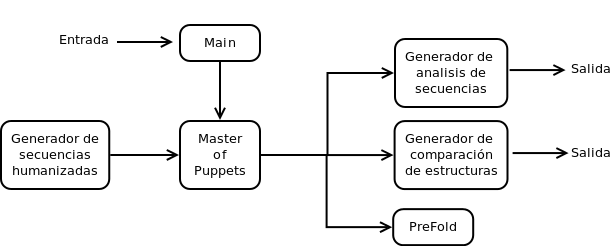
\includegraphics[width=12.5cm, height=5.2cm]{image/componenteRemo.png}
		\caption{Componentes de \textbf{Remo} [2].}
		\label{componentesBasicos}
	\end{center}
\end{figure}

\par En la figura~\ref{arquitecture} se exhibe con más detalle el diseño arquitectónico de \textbf{Remo}.

% \newpage
\begin{figure}[!hbtp]
	\begin{center}
		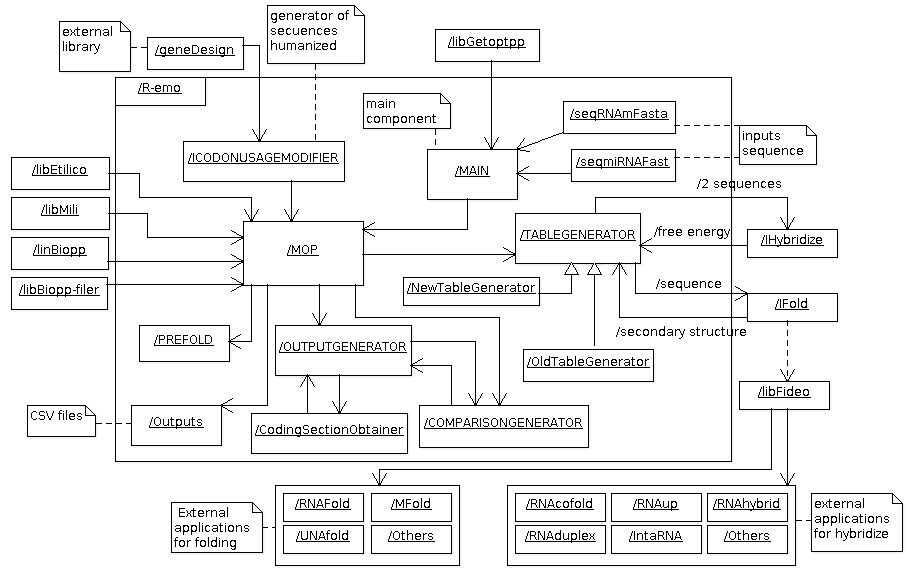
\includegraphics[width=20cm, height=12cm, angle=90]{image/arquitectura.png}
		\caption{UML - Arquitectura del Sistema [2]} 
		\label{arquitecture}
	\end{center}
\end{figure}

\subsection{Catálogo de componentes}
\par A continuación se especifican los distinto componentes de \textbf{Remo}:

\begin{itemize}
	\item \textbf{Main:} punto de entrada de \textbf{Remo}.
	\item \textbf{MOP:} mediador responsable de la comunicación entre los módulos del sistema.

	\item \textbf{CodingSectionObtainer:} permite obtener la mayor sección codificante de una secuencia.

	\item \textbf{TableGenerator:} interfaz para seleccionar el tipo de salida de \textbf{Remo}.

	\item \textbf{OldTableGenerator:} emplea un método ad-hoc usando los backend de folding.

	\item \textbf{NewTableGenerator:} emplea un método formal empleando los backends de hidridacíon.

	\item \textbf{OutputGenerator:} permite obtener los archivos de resultado.

	\item \textbf{ComparisonGenerator:} permite realizar la comparación de estructuras secundarias (parser).

	\item \textbf{Prefold:} permite realizar el folding de las secuencias de $_m$RNA. 
\end{itemize}

\subsection{Comportamiento Dinámico}
En la figura~\ref{compDinamico} se expone un diagrama de secuencia que permite visualizar la interacción dinámica entre los componentes de \remo para el análisis de secuencias de $_m$RNA y $_m$$_i$RNA.

\begin{figure}[!hbtp]
	\begin{center}
		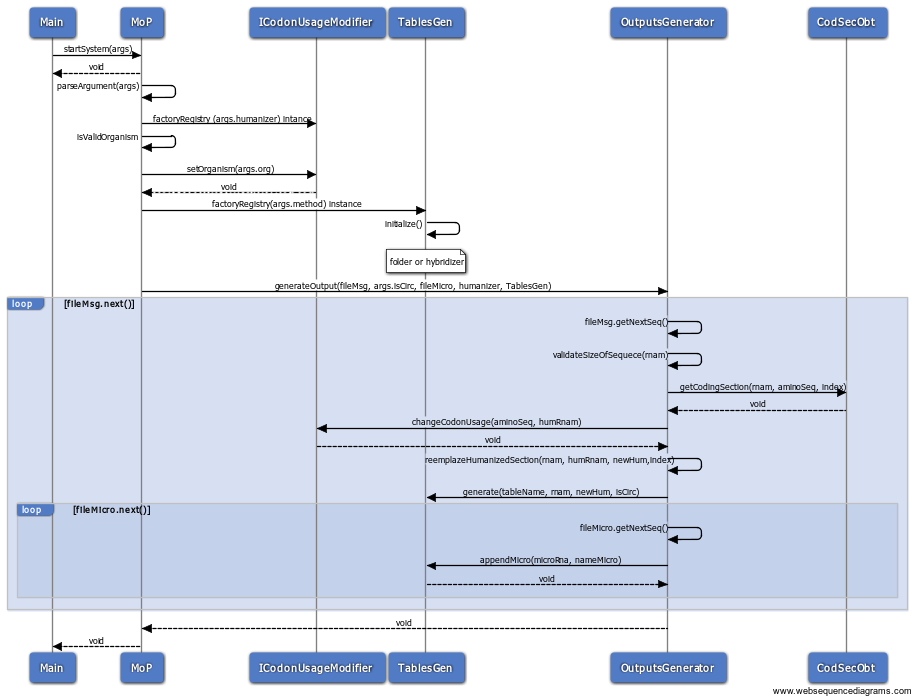
\includegraphics[width=20cm, height=16cm, angle=90]{image/remoCompDin.png}
		\caption{Interacción dinámica entre los componentes de \textbf{Remo} [2].}
		\label{compDinamico}
	\end{center}
\end{figure}

\section{Diseño de Medio Nivel}
\subsection{Diagrama de Paquetes}
\par En la figura~\ref{paquetesDiag} se exhiben el diagrama de paquetes correspondiente a \textbf{Remo}, donde se exhiben las distintas librerías que interactúan.

\begin{figure}[!hbtp]
	\begin{center}
		\vskip 1cm
		\hspace*{1cm}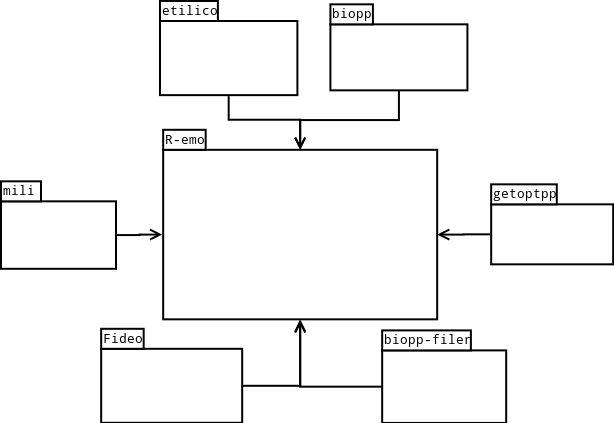
\includegraphics[width=13.5cm, height=10cm]{image/packageDiagramHighGranularity.png}
		\caption{UML - Diagrama de Paquetes [2].}
		\label{paquetesDiag}
	\end{center}
\end{figure}

\subsection{Diagrama de Clases}
\par En la figura~\ref{RemoDClase1} se exhibe un diagrama de clases de \textbf{Remo}. Con el objetivo de lograr una mejor comprensión, se decidió no especificar los métodos y miembros de cada clases. Para mayor detalle puede visitar el apéndice~\ref{disenioEnDetalles} (figuras ~\ref{remoDClase1} y ~\ref{remoDClase2}).

\begin{figure}[!hbtp]
	\begin{center}
		\hspace*{-1.5cm}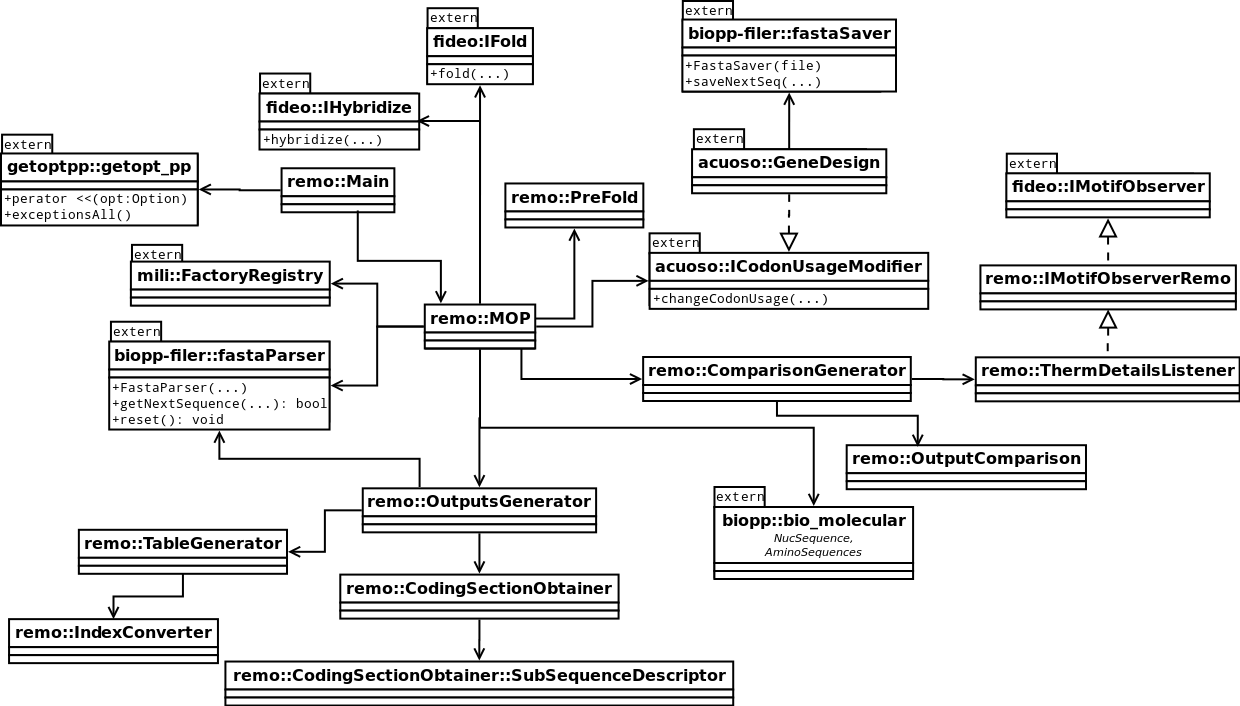
\includegraphics[width=19cm, height=12.5cm, angle=90]{image/emptyClass.png}
		\caption{UML - Diagrama de clases de \textbf{Remo} [2].}
		\label{RemoDClase1}
	\end{center}
\end{figure}

\vskip 15cm
\section{Nuevas Librerías}
\subsection{Fideo: Folding Interface Dynamic Exchange Operations}

\par Tal como se mencionó en la sección~\ref{libreriaAImplementar}, fideo proveerá los servicios necesarios para folding e hibridación. Para tal fin, se empleó el patrón de diseño \emph{Factory Method}(ver Apéndice~\ref{factoryMethod}). Por otra parte, fideo proporciona un parser para identificar motifs en estructuras secundarias. Para tal fin se empleó el patrón de diseño \emph{Observer}(ver Apéndice~\ref{observer}). Para implementar el método \emph{fold()} propiamente dicho se empleó el patrón de diseño \emph{Template Method}(ver Apéndice~\ref{templateMethod}).

En la figura~\ref{interfaceFideo} se exhiben las interfaces implementadas con sus respectivas clases concretas. Se puede observar la interfaz \emph{IMotifObserver} y \emph{IRule} no mencionadas hasta el momento. Básicamente se busca emplear un observer, esto es, fideo proporcionará el parser de estructuras secundarias y establecerá una interfaz la cual deberá ser implementada por \remo para realizar en correspondiente análisis.

\par En este contexto, se puede apreciar la idea del principio de diseño \emph{DIP}. Dado que, si \remo depende de estas interfaces y no de sus respectivas implementaciones se consigue abstraer los detalles de cada librería externa y lograr un software mas versátil. 

\begin{figure}[!hbtp]
	\begin{center}
		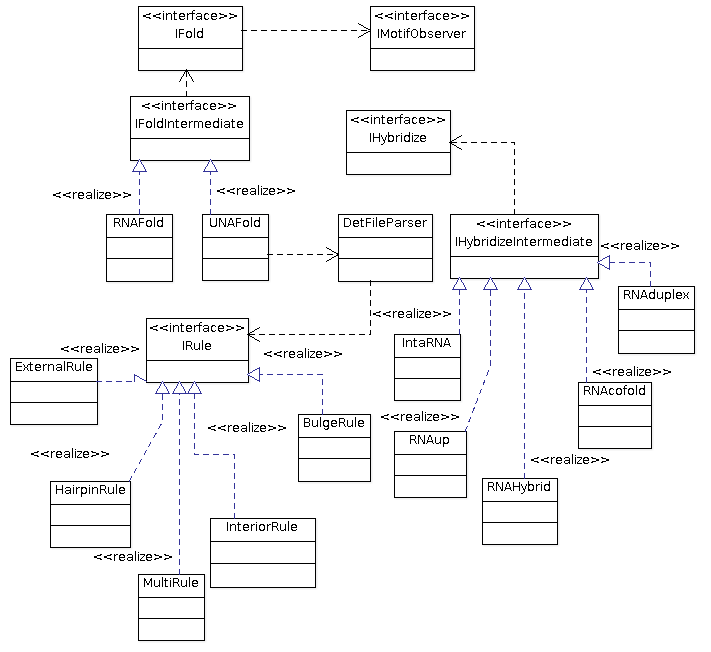
\includegraphics[width=15cm, height=13.5cm]{image/fideoInterface.png}
		\caption{UML - Interfaces de fideo. [2]}
		\label{interfaceFideo} 
	\end{center}
\end{figure}

\par El diagrama de clases correspondiente a fideo puede observarse en la figura~\ref{fideitoDisenio1}. Al igual que en \remo, para lograr una mejor comprensión, se decidió no especificar los métodos y miembros de cada clases, puede visitar el apéndice~\ref{disenioEnDetalles} (figuras~\ref{fideoDisenio1} y ~\ref{fideoDisenio2})para mayor detalle.

\begin{figure}[!hbtp]
	\begin{center}
		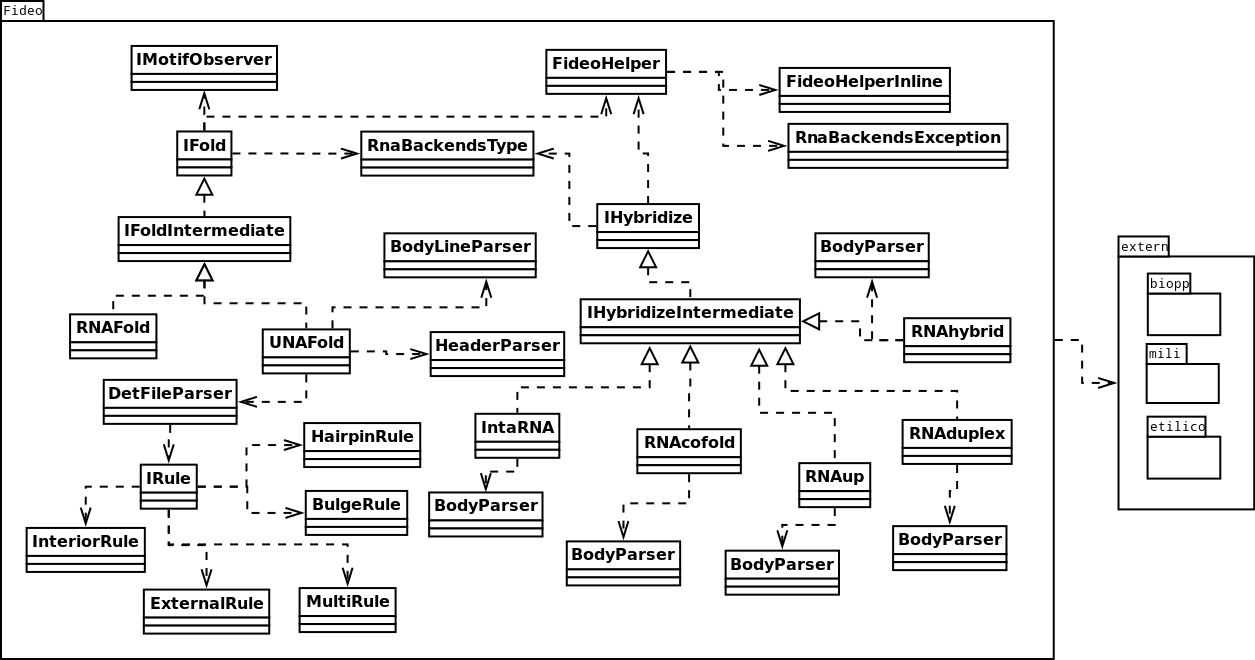
\includegraphics[width=20.5cm, height=13cm, angle=90]{image/clasesFideo.png}
		\caption{UML - Diagrama de clases de fideo [2].}
		\label{fideitoDisenio1}
	\end{center}
\end{figure}

\vskip 10cm
\subsection{Acuoso: Abstract Codon Usage Optimization Software for Organisms}
Esta librería sigue la misma idea de fideo, se definió una interfaz \emph{ICodonUsafeModifier} de modo que sea transparente el uso de cualquier software o método de humanización. En la figura~\ref{acuosoInterface} se observa el diagrama de clases correspondiente.

\begin{figure}[!hbtp]
	\begin{center}
		
\includegraphics[width=15.5cm, height=7.5cm]{image/acuoso.png}
		\caption{UML - Diagrama de clases de Acuoso [2].}
		\label{acuosoInterface}
	\end{center}
\end{figure}

\subsection{Etilico: External Tools Invocation LIbrary COmponent}
\par Etilico corresponde a una librería estática contenedora de diversos métodos necesarios cuyo diseño es muy simple. En la figura~\ref{disenioEtilico} se exhibe el diagrama las clases contenidas en etilico.
\par La clase \emph{Helper} contiene diferentes funciones de gran utilidad. La clase \emph{TmpDirectory}, representa el manejo de directorios temporales, y por último, la clase \emph{Config} se trata de un singletón (ver Apéndice~\ref{singleton}) empleado para configurar las diferentes rutas de las herramientas empleadas.

\begin{figure}[!hbtp]
	\begin{center}
		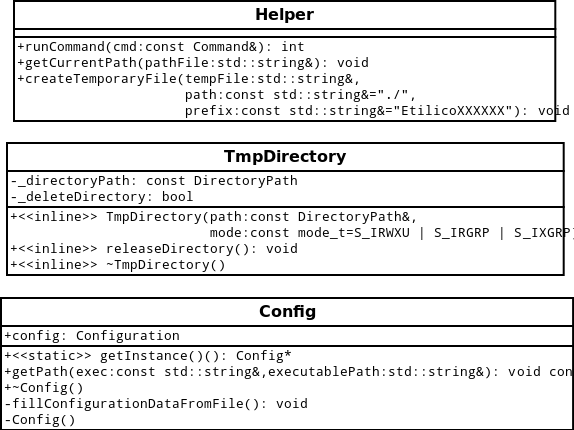
\includegraphics[width=13cm, height=8.5cm]{image/etilico.png}
		\caption{UML - Diagrama de clases de etilico [2].}
		\label{disenioEtilico}
	\end{center}
\end{figure}
   \chapter{Implementación}
\label{implementacion}

\epigraph{Sea lo que sea aquello que cree
o piensa que puede hacer, empiece a hacerlo.
La acción tiene magia, gracia y poder.}%
{\textbf{Goethe}}

El presente capítulo describe algunas características de la puesta a punto de \textbf{Remo}. Se exhibe la representación de datos bioinformáticos, el framework empleado para la distribución de trabajo y algunas porciones de pseudo-código. 

\section{Estructuras y Algoritmos Bioinformáticos}	
\par Ya presentadas las estructuras biológicas básicas en los capítulos anteriores, a continuación se exhibirá la representación de las mismas y algunos algoritmos que son de uso corriente.

\subsection{Representación de nucleótidos, aminoácidos y proteínas}
\par Las cadenas de nucleótidos y de aminoácidos que se utilizaron a lo largo de \textbf{Remo} se representaron como cadenas de caracteres. Denotamos a las mismas como expresiones regulares, las misma se observan a continuación.
	
\begin{itemize}
	\item $nuc\_dna = a \vert t \vert c \vert g $
	\item $nuc\_rna = a \vert u \vert c \vert g  $	
	\item $aminoacido = Ala \vert Arg \vert Asn \vert ...$	
\end{itemize}
	
\par De la misma forma representamos a los genes de DNA, RNA y proteínas.
		
\begin{itemize}
	\item $gen\_dna = (nuc\_dna)^{+}$	
	\item $gen\_rna = (nuc\_rna)^{+}$	
	\item $proteina = aminoacido (aminoacido)^{+}$
\end{itemize}

\subsubsection{Traducción DNA -$>$ RNA}
\par Existe una forma algorítmica de traducir una secuencia de DNA a una secuencia de RNA (Código 7.1). La misma, consiste en analizar cada nucleótido de la cadena cambiando cada $t$ por $u$.

	\begin{lstlisting}[basicstyle=\tt, frame=trBL, tabsize=4,fontadjust=true]
	gen_rna = traslate(gen_dna), donde: 
		
	gen_rna translate(gen_dna) 
	{
	  forall nuc_dna in gen_dna do 
	  {
	    if nuc_dna is t then 
          replace(nuc_dna, u)
	  }
	}	
	\end{lstlisting}
	\hspace*{3.5cm}\caption{Código 7.1: Traducción DNA -$>$ RNA.}

\subsubsection{Traducción RNA -$>$ proteínas}
\par Podemos traducir la secuencia de RNA (compuesta de nucleótidos) a una secuencia de proteínas (compuesta de aminoácidos). Cabe recordar que cada aminoácido se corresponde por tres nucleótidos (un codón).
\par El algoritmo (Código 7.2) toma cada triplete y lo traduce a un aminoácido correspondiente según la tabla de correspondencia observada en la subsección~\ref{molOrg} (figura~\ref{codGen}).
	
\begin{minipage}{\linewidth}
	\begin{lstlisting}[basicstyle=\tt, frame=trBL, tabsize=4,fontadjust=true]
	protein = translate(gen_rna), donde:
		
	protein translate(gen_rna)
	{
	  i = 0
	  triplet = substr(gen_rna, i, 3)
	  while (triplet != STOP && i < length(gen_rna))
	  {
		aminoacid = genetic_code(triplet)			
		protein += aminoacid
		i += 3						    
	    triplet = substr(gen_rna, i, 3)
	  }
	}
	\end{lstlisting}
\end{minipage}
\hspace*{3.5cm}\caption{Código 7.2: Traducción RNA -$>$ proteínas.}

\section{Decisiones de Implementación}
\subsection{Implementar vs. Integrar}

\par Ante el requerimiento de contar con algoritmos para el cálculo de la estructura secundaria de RNA, se evaluó entre implementar completamente los algoritmos o integrar/adaptar los algoritmos existentes.

\par En este sentido, las interfaces propuestas no descartan ninguna de las dos posibilidades, sino simplemente especifican los ``servicios'' que deben ofrecer al sistema las eventuales implementaciones, ya sean propias o ajenas.

\par Por otro lado, implementar este tipo de algoritmos requiere un profundo conocimiento del dominio (Química Molecular). Además, debido a la complejidad de los mismos, se requieren validaciones empíricas para demostrar la fidelidad de los resultados lo cual excedía el alcance de este trabajo.

\par Finalmente se optó por integrar al sistema los algoritmos para implementar las respectivas interfaces. A continuación se exhibe dicha relación.

\begin{tabbing}
\hspace*{6.5cm} \= \hspace*{5cm} \kill
\hspace*{1cm} \textbf{Interface} \> \textbf{Algortimos} \\
\hspace*{.9cm} fideo::IFold \> UNAFold, RNAFold \\      
\hspace*{1cm}fideo::IHybridize \> RNAup, IntaRNA, RNAcofold, \\
\hspace*{6.6cm}RNAduplex, RNAHybridize \\
\hspace*{1cm}acuoso::ICodonUsageModifier \> GeneDesign \\
\end{tabbing}

\subsection{Método Ad-hoc}
\par En primer instancia, para realizar las comparaciones necesarias de $_m$RNA y $_m$$_i$RNA se empleó un método ad-hoc cumpliendo con los requerimientos definidos.
\par Básicamenta la idea consistió en fijar cada secuencia de $_m$RNA y por cada secuencia de $_m$$_i$RNA, ir desplazándola de a un nucleótido por vez en el mensajero desde la posición inicial. En cada paso, se realizaron los análisis correspondientes.
\par Esta manera de implementar las pasadas de $_m$$_i$RNA sobre los $_m$RNA es ineficiente (Código 7.3). Sin embargo, se escogió adrede esta implementación debido a los siguientes motivos:
\begin{itemize}
	\item Rápido de implementar y testear (*).
	\item Se conocía que el cuello de botella de performance no iba a estar ahí (que tiene O(n$^2$) pero de un N muy chico, 22 nucleótidos aproximadamente que es el tamaño medio de los $_m$$_i$RNA), sino en el folding que es O(n$^3$), con un N dos órdenes de magnitud superior al de las $_m$$_i$RNA.
\end{itemize}

\par (*) Este principio lo cita Donald Knuth\footnote{Donald Ervin Knuth, es uno de los más reconocidos expertos en Ciencias de la Computación por su fructífera investigación dentro del análisis de algoritmos y compiladores. Es Profesor Emérito de la Universidad de Stanford.}, diciendo \emph{``premature optimizations are the mother of all evils''}, lo cual significa que \emph{optimizar antes de tener algo andando, es básicamente la madre de todos los males}.

\par Por otro lado, para que sea O(n), la manera es ir desplazando el $_m$$_i$RNA pero en vez de recorrerlo cada vez que se avanza un nucleótido en el mensajero, solamente sacarle el nucleótido que se descarta, y agregarle el nucleótido que entra. De esta manera, el ciclo completo se hace una sola vez, y luego se opera dos veces por cada desplazamiento (una para el nucleótido que se va y otra para el que entra). Implementarlo de esta manera requería una estructura de todo el programa mucho menos imperativa/secuencial, sino que había que hacer una especie de pipeline como tienen los microprocesadores.

\begin{minipage}{\linewidth}
	\begin{lstlisting}[basicstyle=\tt, frame=trBL, tabsize=4,fontadjust=true]
	try
	{
		Para todo mRNA
		{
			validar secuencia
			obtener mayor seccion codificante
			humanizar mayor seccion codificante
			restablecer secuencia original

			generar archivo de salida
			Para todo miRNA
			{
				obtener nombre de miRNA
				agregar comparaciones al archivo
			}
			restablecer miRNA
		}
	}
	catch (...)
	{
		...
	}
	\end{lstlisting}
\end{minipage}
\hspace*{3cm}\caption{Código 7.3: Pseudo-código $_m$RNA vs. $_m$$_i$RNA.}

\subsection{Formalizando}
\par Luego de analizar los resultados intermedios que se obtuvieron con el método Ad-hoc, se concluyó que el problema es mucho más grande de lo que se pensaba inicialmente, con lo que, nuestra aproximación era demasiada poco precisa, aunque como primer aproximación sirvió. 
\par Por tal motivo se comenzaron a emplear herramientas más avanzadas, como los son las herramientas de hibridación (subsection~\ref{hibrid}), dado que las mismas cuentan con validaciones empíricas y son confiables.

\section{El Framework FuD}
\par Con el objetivo de distribuir el trabajo en diversos nodos de computación para lograr menores tiempos de espera en los resultado se decidió emplear el framework \textbf{FuD} (del acrónico \emph{FuDePAN ubiquitous Distribution}). \textbf{FuD} es un framework para la distribución de trabajos, o un framework para la implementación de aplicaciones distribuídas\cite{clus09}. Como tal, no depende del problema a implementar y no fuerza ningún modelo de comunicación o disposición de las unidades de procesamiento que serán utilizadas. 
\par En términos generales, \textbf{FuD} se organiza como un esquema \emph{Master-Worker} (un servidor y varios clientes conectados al mismo). Tanto cliente como servidor, se encuentran organizados en tres niveles bien separados (figura~\ref{disenioFud}), cada uno de ellos con una única responsabilidad claramente definida. La comunicación entre los diferentes niveles se encuentra estrictamente limitada, es decir, por cada nivel existe un único punto de comunicación ya sea para comunicarse con la capa superior o con la inferior. Cuando un mensaje es creado, éste debe atravesar las diferentes capas comenzando desde la de nivel más alto hacia la capa inferior, y luego recorrer en sentido contrario las capas del lado. En el apéndice~\ref{detFud} se decriben brevemencte cada una de las capas que conforman este framework.

\begin{figure}[h!] \hspace{.60cm}
    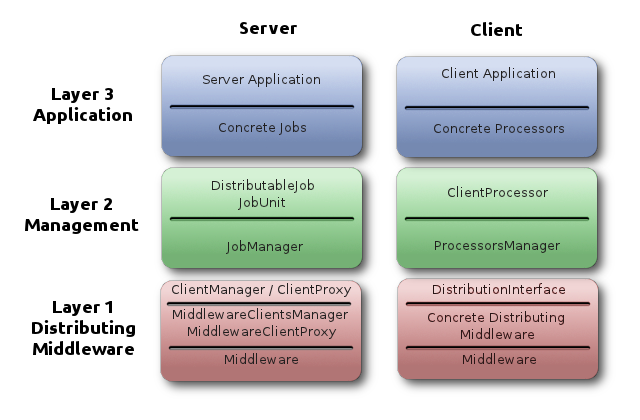
\includegraphics[scale=.55]{image/AbstractLayers.png}
    \caption{Vista abstracta de las capas de \textbf{FuD} [16].} 
    \label{disenioFud}
\end{figure}

\subsection{Conceptos Importantes}
Los siguientes conceptos son necesarios para entender el funcionamiento de una aplicación que usa FuD:
\begin{itemize}
	\item \emph{Cliente:} un cliente es una aplicación conectada al servidor y es el encargado de realizar las tareas de procesamiento.
 	\item \emph{Trabajo:} un trabajo es cualquier tarea a realizar por la aplicación (también llamado trabajo distribuíble). Los mismos se
 						  pueden subdividir en unidades de trabajo.
 	\item \emph{Unidad de Trabajo:} representa un cómputo concreto y pertenece a un trabajo particular. No se puede dividir.
 	\item \emph{Manejador de clientes:} módulo encargado de manejar los clientes conectados al servidor.
 	\item \emph{Manejador de trabajos:} módulo de \textbf{FuD} encargado de llevar cuenta de los trabajos (de ambos tipos) que maneja el
 										framework en un momento dado.
 \end{itemize}

\par Como se mencionó anteriormente el cuello de botella en cuanto a complejidad se encuentraba en el folding de las secuencias. Las implementaciones del algoritmo de Zuker (UNAFold y RNAFold) no son distribuibles naturalmente, es decir, no es lo mismo foldear una secuencia completa que, dividirla en tramos, foldear cada uno de los tramo, y unificar los resultados. Por lo cual, el trabajo que se distribuye es el folding de secuencias (original y humanizada), es decir, cada nodo será encargado de foldear cierta secuencia. 
Dado a que \remo necesitaba ser puesto a prueba con un gran número de secuencias para que los resultados sean fiables y consistentes, el uso de \textbf{FuD} benefició notoriamente los tiempo de espera de resultados.

\section{Métricas de Código}
\par Para analizar el código estáticamente se usaron herramientas como CLOC\footnote{http://cloc.sourceforge.net/} (Count Lines of Code) y CCCC\footnote{http://cccc.sourceforge.net/} (\textbf{\textit{C}} and \textbf{\textit{C++}} Code Counter). En esta sección se describen métricas de código generales obtenidas por ambas herramientas y se analizan los resultados obtenidos.

\subsection{Métricas de R-emo}
\par \textbf{Remo} esta compuesto por 21 archivos con 3002 líneas de texto a la fecha de publicación del presente documento, dicha cantidad puede variar en el tiempo debido a posibles modificaciones, extensiones o mantenimiento.

\par El cuadro \ref{clocRemo} resume los resultados obtenidos después de correr la herramienta CLOC sobre los archivos de \textbf{Remo}.

\begin{table}[!htf]
    \begin{center}
    \begin{tabular}{|l|r|r|r|r|c|}
    \hline
    \multicolumn{2}{|c|}{Files} & \multicolumn{3}{|c|}{Line Types} & \hspace{0.2cm}\% \\
    \hline
    \textbf{Type} & \textbf{Count} & \textbf{Blank} & \textbf{Comment} & \textbf{Source} & \small{\textbf{\#Comms./Tot.}}\\
    \hline
    \texttt{C++ source} & 10 & 161 & 553 & 1108 & 33.2 \\
    \hline
    \texttt{C++ header} & 11 & 150 & 757 & 273 & 73.4 \\
    \hline
    \textbf{Total}      & 21 & 311 & 1310 & 1381 & 48.6 \\
    \hline
    \end{tabular}
    \caption{Resultados de CLOC para \textbf{Remo} [2].}
    \label{clocRemo}
    \end{center}
\end{table}

\par La herramieta CCCC proporciona un reporte completo sobre las métricas de código, incluyendo métricas de diseño Orientado a Objetos y todo tipo de información relevante en cuanto a código. Un análisis exhaustivo de los resultados de estas métricas se encuentra fuera del alcance del presente trabajo, por lo cual en el cuadro \ref{ccccRemo} se muestra un pequeño resúmen de los mismos.

\begin{table}[!htf]
    \begin{center}
	\begin{tabular}{|c|c|c|c|}
	\hline 
	Metric &Tag &Overall &Per Module \\
	 \hline 
	Number of modules &NOM & 31 &  \\
	 \hline 
	Lines of Code &LOC & 342 &11.032 \\
	 \hline 
	McCabe's Cyclomatic Number &MVG & 8 & 0.258 \\
	 \hline 
	Lines of Comment &COM & 787 & 25.387 \\
	 \hline 
	LOC/COM &L\_C & 0.435 &  \\
	 \hline 
	MVG/COM &M\_C & 0.010 &  \\
	 \hline 
	Information Flow measure (  inclusive ) &IF4 & 0 & 0 \\
	 \hline 
	Information Flow measure (  visible ) &IF4v & 0 & 0 \\
	 \hline 
	Information Flow measure (  concrete ) &IF4c & 0 & 0 \\
	 \hline 
	Lines of Code rejected by parser &REJ & 49 &  \\
	 \hline 
	\end{tabular} 
	\caption{Resultados de CCCC para \textbf{Remo} [2].}
	\label{ccccRemo}
\end{center}
\end{table}

\par Para una descripción de Número Ciclomático de McCabe ver ~\cite{McCabe}. 

\subsection{Métricas de Fideo}
\par \textbf{Fideo} esta compuesto por 30 archivos con 3540 líneas de texto a la fecha de publicación del presente documento, dicha cantidad puede variar en el tiempo debido a posibles modificaciones, extensiones o mantenimiento.

\par El cuadro \ref{clocFideo} resume los resultados obtenidos después de correr la herramienta CLOC sobre los archivos de fideo.

\begin{table}[!htf]
    \begin{center}
    \begin{tabular}{|l|r|r|r|r|c|}
    \hline
    \multicolumn{2}{|c|}{Files} & \multicolumn{3}{|c|}{Line Types} & \hspace{0.2cm}\% \\
    \hline
    \textbf{Type} & \textbf{Count} & \textbf{Blank} & \textbf{Comment} & \textbf{Source} & \small{\textbf{\#Comms./Tot.}}\\
    \hline
    \texttt{C++ source} & 10   &    161  &     344   &    967 & 26.2 \\
    \hline
    \texttt{C++ header} & 20   &    243  &    1222   &    603 & 66.9 \\
    \hline
    \textbf{Total}      &  30  &     404 &     1566  &    1570 & 49.9 \\
    \hline
    \end{tabular}
    \caption{Resultados de CLOC para fideo [2].}
    \label{clocFideo}
    \end{center}
\end{table}

\subsection{Métricas de Acuoso}
\par \textbf{Acuoso} esta compuesto por 7 archivos con 663 líneas de texto a la fecha de publicación del presente documento, dicha cantidad puede variar en el tiempo debido a posibles modificaciones, extensiones o mantenimiento.

\par El cuadro \ref{clocAcuoso} resume los resultados obtenidos después de correr la herramienta CLOC sobre los archivos de acuoso.

\begin{table}[!htf]
    \begin{center}
    \begin{tabular}{|l|r|r|r|r|c|}
    \hline
    \multicolumn{2}{|c|}{Files} & \multicolumn{3}{|c|}{Line Types} & \hspace{0.2cm}\% \\
    \hline
    \textbf{Type} & \textbf{Count} & \textbf{Blank} & \textbf{Comment} & \textbf{Source} & \small{\textbf{\#Comms./Tot.}}\\
    \hline
    \texttt{C++ source} & 2 & 26 & 72 & 160 & 31 \\
    \hline
    \texttt{C++ header} & 5 & 46 & 247 & 112 & 68 \\
    \hline
    \textbf{Total}      & 7 & 72 & 319 & 272 & 53 \\
    \hline
    \end{tabular}
    \caption{Resultados de CLOC para acuoso [2].}
    \label{clocAcuoso}
    \end{center}
\end{table}

\subsection{Métricas de Etilico}
\par \textbf{Etilico} esta compuesto por 8 archivos con 624 líneas de texto a la fecha de publicación del presente documento, dicha cantidad puede variar en el tiempo debido a posibles modificaciones, extensiones o mantenimiento.

\par El cuadro \ref{clocEtilico} resume los resultados obtenidos después de correr la herramienta CLOC sobre los archivos de etilico.

\begin{table}[!htf]
    \begin{center}
    \begin{tabular}{|l|r|r|r|r|c|}
    \hline
    \multicolumn{2}{|c|}{Files} & \multicolumn{3}{|c|}{Line Types} & \hspace{0.2cm}\% \\
    \hline
    \textbf{Type} & \textbf{Count} & \textbf{Blank} & \textbf{Comment} & \textbf{Source} & \small{\textbf{\#Comms./Tot.}}\\
    \hline
    \texttt{C++ source} & 2 & 18 & 67 & 145 & 31.6 \\
    \hline
    \texttt{C++ header} & 6 & 64 & 260 & 152 & 63.1 \\
    \hline
    \textbf{Total}      & 8 & 82 & 327 & 297 & 52.4 \\
    \hline
    \end{tabular}
    \caption{Resultados de CLOC para etilico [2].}
    \label{clocEtilico}
    \end{center}
\end{table}

\subsection{Métricas de Remo Fudizado}
\subsubsection{Server}
\par \textbf{Remo server} esta compuesto por 8 archivos con 803 líneas de texto a la fecha de publicación del presente documento, dicha cantidad puede variar en el tiempo debido a posibles modificaciones, extensiones o mantenimiento.

\par El cuadro \ref{clocServer} resume los resultados obtenidos después de correr la herramienta CLOC sobre los archivos correspondientes a remo server.

\begin{table}[!htf]
    \begin{tabular}{|l|r|r|r|r|c|}
    \hline
    \multicolumn{2}{|c|}{Files} & \multicolumn{3}{|c|}{Line Types} & \hspace{0.2cm}\% \\
    \hline
    \textbf{Type} & \textbf{Count} & \textbf{Blank} & \textbf{Comment} & \textbf{Source} & \small{\textbf{\#Comms./Tot.}}\\
    \hline
    \texttt{C++ source} & 4 & 59 & 143 & 387 & 0.36 \\
    \hline
    \texttt{C++ header} & 4 & 45 & 129 & 144 & 0.47 \\
    \hline
    \textbf{Total}      & 8 & 104 & 272 & 531 & 0.33 \\
    \hline
    \end{tabular}
    \caption{Resultados de CLOC para remo server [2].}
    \label{clocServer}
\end{table}

\subsubsection{Client}
\par \textbf{Remo client} esta compuesto por 4 archivos con 285 líneas de texto a la fecha de publicación del presente documento, dicha cantidad puede variar en el tiempo debido a posibles modificaciones, extensiones o mantenimiento.

\par El cuadro \ref{clocClient} resume los resultados obtenidos después de correr la herramienta CLOC sobre los archivos correspondientes a un remo client.

\begin{table}[!htf]
    \begin{center}
    \begin{tabular}{|l|r|r|r|r|c|}
    \hline
    \multicolumn{2}{|c|}{Files} & \multicolumn{3}{|c|}{Line Types} & \hspace{0.2cm}\% \\
    \hline
    \textbf{Type} & \textbf{Count} & \textbf{Blank} & \textbf{Comment} & \textbf{Source} & \small{\textbf{\#Comms./Tot.}}\\
    \hline
    \texttt{C++ source} & 2 & 24 & 68 & 94 & 0.41 \\
    \hline
    \texttt{C++ header} & 2 & 21 & 84 & 39 & 0.68 \\
    \hline
    \textbf{Total}      & 4 & 45 & 152 & 133 & 0.46 \\
    \hline
    \end{tabular}
    \caption{Resultados de CLOC para un remo client [2].}
    \label{clocClient}
    \end{center}
\end{table}
\subsection{Análisis de las Métricas}
\par Un dato particularmente interesante sobre los resultados de CLOC, es la cantidad de líneas de comentarios y su porcentaje con respecto al total de líneas de código efectivas. La siguiente fórmula describe la relación comentarios/código y la misma fue usada para calcular la última columna de la tablas exhibidas anteriormente:

$$\frac{\#comment\_lines}{\#comment\_lines + \#code\_lines}$$

\vskip .5cm
\par Este valor ronda aproximadamente el 0.50, lo que significa que hay casi la misma cantidad de líneas de comentarios que líneas de código. Este porcentaje de líneas de comentarios se debe, en mayor medida, a que por cada archivo (por más pequeño que sea) se incluye una cabecera (``header'') definiendo ciertos detalles del archivo tal como se observa en el cuadro~\ref{remoComment}.

\begin{table}[!h]
    \lstset{language=C++}
    \begin{lstlisting}[frame=single]
/**
* @file     CodingSectionObtainer.h
* @brief    CodingSectionObtainer provides the 
*           interface that allows get the coding
*           section of sequence
*
* @author Franco Riberi
* @email  fgriberi AT gmail.com
*
* Contents:  Header file for remo providing class 
*            CodingSectionObtainer.
*
* System:    remo: RNAemo - RNA research project
* Language:  C++
*
* @date      October 2012
*
* This file is part of remo.
*
* Copyright (C) 2012 - Franco Riberi, FuDePAN.
*
* Remo is free software: you can redistribute it and/or 
* modify it under the terms of the GNU General Public 
* License as published by the Free Software Foundation, 
* either version 3 of the License, or (at your option)
* any later version.
*
* Remo is distributed in the hope that it will be useful
* but WITHOUT ANY WARRANTY; without even the implied 
* warranty of MERCHANTABILITY or FITNESS FOR A 
* PARTICULAR PURPOSE. See the GNU General Public 
* License for more details.
*
* You should have received a copy of the GNU General 
* Public License along with Remo. If not, see
* <http://www.gnu.org/licenses/>.
*/
    \end{lstlisting}
    \centering \caption{Comentario Doxygen de encabezado de archivo en \textbf{Remo} [2].}
    \label{remoComment}
\end{table}

\par Para justificar más la alta cantidad de comentarios, todo componente de software, sean estos clases, estructuras, funciones, atributos, etcétera, tiene una descripción detallada a ser interpretada por \textit{Doxygen} (el cuál incluye perfiles de funciones) para la generación de documentación automática. El ejemplo~\ref{remoComment} muestra la notación utilizada para Doxygen exhibiendo además el porqué de la alta tasa de comentarios.

\begin{table}[!h]
    \lstset{language=C++}
    \begin{lstlisting}[frame=single]
/** @brief Get the coding section
*
* Method for obtaining the largest coding section of a 
* given sequence.
* @param src:     original sequence
* @param dest:    larger coding section
* @param posInit: to fill with the starting position 
*                 of the largest coding section
* @return void
*/
void getCodingSection(const biopp::NucSequence& src, 
                      biopp::AminoSequence& dest, 
                      size_t& posInit);
    \end{lstlisting}
    \centering \caption{Comentario Doxygen de una función en \textbf{Remo} [2].}
    \label{remoComment}
\end{table}
   \chapter{Experimentación y Testing}

\epigraph{No solamente el aprendizaje vulgar, sino
también el científico esta sometido pues, a ensayo
y error.}%
{\textbf{Saturdino de la Torre}}

Las pruebas de software tienen por objetivo proporcionar información objetiva e independiente sobre la calidad del producto. Son una actividad más en el proceso de control de calidad. Dependiendo del tipo de pruebas, estas actividades podrán ser implementadas en cualquier momento del proceso de desarrollo. Las pruebas deben ser independientes, repetibles, portátiles y reutilizables. 

\section{Google C++ Testing Framework}

\par El framework \emph{googletest}, también conocido como \emph{gtest}, se empleó para escribir las pruebas de todo el código implementado, tanto de \remo como del resto de las librerías ya mencionadas. 
\par Básicamente soporta detección automática de pruebas, posee un amplio conjunto de aserciones, permite definir aserciones al usuario, generación de reportes XML respecto de los test, entre otras cosas.

\par Este framework aísla las pruebas mediante la ejecución de cada una de ellas en un objeto diferente. Cuando una prueba falla, \emph{gtest} permite correrla de forma aislada para la depuración rápida. 

\par Se trata de escribir test mediante el uso de aserciones, es decir, declaraciones que comprueban si una condición es verdadera, o falsa. Una afirmación del resultado puede llevar a un éxito, un fracaso no fatal o un fracaso fatal. Si se produce un fallo fatal, se aborta la función actual, de lo contrario el programa continúa normalmente.

En el Cuadro~\ref{aserciones} se exhiben las aserciones básicas y algunas aserciones binarias:

\begin{table}[!hbt]
	\begin{center}
		\begin{tabular}{|l|l|l|}
			\hline
			Fatal assertion & Nonfatal assertion & Verifies \\
			\hline
			ASSERT\_TRUE(cond) & EXPECT\_TRUE(cond) & cond == True\\ \hline
			ASSERT\_FALSE(cond) & EXPECT\_FALSE(cond) & cond == False\\ \hline
			ASSERT\_EQ(exptd, actual) & EXPECT\_EQ(exptd, actual) & exptd == actual\\ \hline
			ASSERT\_NE(val1, val2) &	EXPECT\_NE(val1, val2) &	val1 $!=$ val2\\ \hline
			ASSERT\_LT(val1, val2) &	EXPECT\_LT(val1, val2) & val1 $<$ val2\\ \hline
			ASSERT\_LE(val1, val2) &	EXPECT\_LE(val1, val2) &	val1 $<=$ val2\\ \hline
			... & ... & ...\\ \hline
		\end{tabular}
		\caption{Aserciones test en \emph{gtest} [2].}
		\label{aserciones}
	\end{center}
\end{table}

Cuando fallan, ASSERT\_* produce un fallo fatal y regresa de la función actual, mientras que EXPECT\_* no produce un fallo fatal, lo que permite que la función continue en funcionamiento. En cualquiera de los casos, un error de aserción significa la presencia de un error.

\par En el Cuadro~\ref{test} se puede observar un ejemplo de prueba empleando gtest.

\begin{table}[!h]
    \lstset{language=C++}
    \begin{lstlisting}[frame=single]
TEST(UnaFoldBackendTestSuite1, BasicTest)
{
    const std::string sequence = "AAGGGCT...";
    const biopp::NucSequence seq(sequence);
    biopp::SecStructure secStructure;

    IFold* p = Fold::new_class("UNAFold");
    ASSERT_TRUE(p != NULL);

    EXPECT_NO_THROW(p->fold(seq, true, secStructure));
    delete p;

    EXPECT_EQ(32, secStructure.size());
    EXPECT_TRUE(secStructure.is_circular());

    EXPECT_FALSE(HelperTest::checkDirTmp());
}

    \end{lstlisting}
    \centering \caption{Ejemplo gtest [3].}
    \label{test}
\end{table}

\par La regla de oro es usar EXPECT\_* cuando se desea que la prueba continue revelando más errores después del error de la aserción, y utilizar ASSERT\_* cuando continuar tras el fracaso no tiene sentido.

\par Por ejemplo, la aserción de segundo test: ASSERT\_TRUE (p != NULL) en el Cuadro~\ref{test} tiene sentido, ya que se necesita una referencia al backend, si esto no pasara daría lugar a una violación de segmento cuando p es NULL.

\par Después de definir las diferentes pruebas, se ejecutan con RUN\_ALL\_TESTS(), que devuelve 0 si todas las pruebas tienen éxito, o 1 en caso contrario. Cuando se invoca, los RUN\_ALL\_TESTS() sucede lo siguiente:

\begin{enumerate}
	\item guarda el valor de los flags de prueba.
	\item gtest construye los objetos necesarios.
	\item inicializa los objetos mediante setUp().
	\item ejecuta las pruebas.
	\item limpia las pruebas, es decir, destruye los objetos empleados mediante TearDown().
	\item restablece los flags con los valores almacenados inicialmente.
	\item repite todos los pasos hasta que se hayan ejecutado todas las pruebas.
\end{enumerate}

Para mayor información puede visitar \url{https://code.google.com/p/googletest/}.

\section{Cobertura de Código}
\par Se trata de una medida cuantitativa utilizada en pruebas de software que describe el grado de código fuente testeado, lo cuál funciona como una medida indirecta de calidad. Como la cantidad de tests necesarios para garantizar el correcto funcionamiento para todos los \textit{inputs} posibles suele ser demasiado grande, se eligen casos especialmente representativos. 
\par La cobertura de las pruebas fue realizada empleando la herramienta gcov\footnote{http://gcc.gnu.org/onlinedocs/gcc/Gcov.html}. 
\par En las tablas~\ref{coberturaFideo},~\ref{coberturaAcuoso} y~\ref{coberturaEtilico} se muestran las cobertura de código correspondientes a fideo, acuoso y etilico respectivamante.

\begin{table}[!htf]
    \begin{center}
    \begin{tabular}{|l|r|r|c|}
        \hline
        & \textbf{Hit} & \textbf{Total} & \textbf{Coverage \%} \\
        \hline
        Lines & 666 & 751 & 88.7 \\
        \hline
        Functions & 153 & 218 & 70.2 \\
        \hline
        Branches & 882 & 1750 & 46.9 \\
        \hline            
    \end{tabular}
    \caption{Cobertura Fideo [2].}
    \label{coberturaFideo}
    \end{center}
\end{table}

\begin{table}[!htf]
    \begin{center}
    \begin{tabular}{|l|r|r|c|}
        \hline
        & \textbf{Hit} & \textbf{Total} & \textbf{Coverage \%} \\
        \hline
        Lines & 108 & 134 & 80.6 \\
        \hline
        Functions & 26 & 59 & 44.1 \\
        \hline
        Branches & 141 & 353 & 39.9 \\
        \hline            
    \end{tabular}
    \caption{Cobertura acuoso [2].}
    \label{coberturaAcuoso}
    \end{center}
\end{table}

\begin{table}[!htf]
    \begin{center}
    \begin{tabular}{|l|r|r|c|}
        \hline
        & \textbf{Hit} & \textbf{Total} & \textbf{Coverage \%} \\
        \hline
        Lines & 36 & 88 & 40.9 \\
        \hline
        Functions & 10 & 41 & 24.4 \\
        \hline
        Branches & 40 & 216 & 18.5 \\
        \hline            
    \end{tabular}
    \caption{cobertura etilico.}
    \label{coberturaEtilico}
    \end{center}
\end{table}
    
%III Conclusiones
\part{Conclusiones}
    \chapter{Conclusiones del Trabajo}

\epigraph{Pones tu pie en el camino y si no cuidas
tus pasos, nunca sabes a donde te pueden
llevar.}%
{\textbf{John Ronald Reuel Tolkien}}

\section{Resultados}
\textcolor{red}{complete}
Informar los datos con que se corrio finalmente

\section{Conclusión Final}
\textcolor{red}{complete}

\section{Logros}
Este proyecto de trabajo final fue presentado previamente en dos oportunidades:
\begin{itemize}
    \item \emph{\textbf{Relationship between divergence of using synonymous codons in host-virus and the presence of microRNA.}} Franco	Riberi, Laura Tardivo, Lucia Fazzi, Guillermo Biset, Daniel Gutson, Daniel Rabinovich. En 3CAB$^{2}$C (3er. Congreso Argentino de Bioinformática y Biología Computacional).

    \item \emph{\textbf{Estudio de la relación entre divergencia  en el uso de codones del virus respecto al huésped y reconocimiento por los microRNA.}} Riberi F, Fazzi L, Tardivo L, Gutson D, Rabinovich D. En XXXII Reunión Científica Anual (SAV2012-Sociedad Argentina de Virología).    
\end{itemize}

Además, \textbf{Remo} fue abalado por Secretaria de Ciencia y Técnica de la UNRC otorgando la beca TICs para la finalización de carrera.

\section{Aportes}
\par A FuDePAN:
\begin{itemize}
    \item Fideo   : \url{fideo.googlecode.com}
    \item Acuoso  : \url{acuoso.googlecode.com}
    \item Etilico : \url{etilico.googlecode.com}
    \item Otras   : aportes en otras librerias tales como mili\url{mili.googlecode.com} y biopp\url{biopp.googlecode.com}.
\end{itemize}

\par A la comunidad científica:
\par El principal aporte de este trabajo fue el análisis y la formalización del
problema biológico y la posterior propuesta de cómo solucionarlo
computacionalmente. 

\par Por otra parte, de alguna manera esto pretende ser un aporte al trabajo interdisciplinario como forma de aplicar los conocimientos científicos en la resolución concreta de problemas que afectan la calidad de vida de las personas.

\section{Trabajos Futuros}
\begin{itemize}
	\item Agregar nuevos backends para folding en \emph{fideo}.
	\item Agregar nuevos backends para hibridización en \emph{fideo}.
	\item Agregar nuevos backends para la humanización en \emph{acuoso}.
	\item Implementar un módulo de control de marco de lectura de las secuencias.
	\item Realizar el mismo estudia aplicado a proteínas.
\end{itemize}

\section{Repositorio del sistema}
Se puede acceder al código fuente de este proyecto y a su documentación visitando \url{http://r-emo.googlecode.com}.




%%---------------- Bibliografía -------------------------------------------- 
\addcontentsline{toc}{chapter}{Bibliografía}
\nocite{*}
\bibliographystyle{apalike}
\bibliography{tex/biblio}

\newpage{}
\section*{\Large{\textbf{Fuente de Imágenes}}}
\textcolor{buscar buenas fuentes, confiables}

\par [1] Estructura de una célula:  \url{https://www.google.com.ar/search?q=} 
\par \hspace*{.5cm}\url{estructura+de+una+celula.}

\par [2] Elaboración propia. 

\par [3] Taxonomía de las especies. \url{http://www.ceibal.edu.uy/UserFiles/}
\par \hspace*{.5cm}\url{P0001/ODEA/ORIGINAL/BIOPELIGRO.elp/tax.jpg} 

\par [4] Estructura de un Nucleótido. \url{http://www.cobach-elr.com/academias/}
\par \hspace*{.5cm}\url{quimicas/biologia/biologia/curtis/libro/img/3-29.jpg} 

\par [5] Código genético. \url{http://ciencias4eso.byethost22.com/Joomla/images/} 
\par \hspace*{.5cm}\url{stories/codigo.gif}

\par [6] Cadenas antiparalelas. \url{http://genemol.org/biomolespa/}
\par \hspace*{.5cm}\url{la-molecula-de-adn/adn-01.jpg}

\par [7] Molécula de RNA y DNA. \url{https://upload.wikimedia.org/wikipedia/} 
\par \hspace*{.5cm}\url{commons/thumb/0/0e/Difference_}
\par \hspace*{.5cm}\url{DNA_RNA-ES.svg/450px-Difference_DNA_RNA-ES.svg.png}

\par [8] Estructura molecular de las proteínas. \url{http://4.bp.blogspot.com/}
\par \hspace*{.5cm}\url{\_4ww6723C4UE/TBbKBSF-6xI/AAAAAAAAAE0/12M_6XTEU88/s1600}
\par \hspace*{.5cm}\url{/estructuraproteinasbl9.png}

\par [9] Estructura secundaria del DNA. \url{http://o.quizlet.com/}
\par \hspace*{.5cm}\url{FQEKPJNVM3YIdzpH7yR93g.png}
	
\par [10] Replicación semi conservativa. \url{http://html.rincondelvago.com/}
\par \hspace*{.7cm}\url{000769161.png}

\par [11] El Dogma Central. \url{http://www.cbs.dtu.dk/staff/dave/}
\par \hspace*{.7cm}\url{transcript_transl.gif}

\par [12] Transcripción del RNA. \url{http://3.bp.blogspot.com/_nZqQMbHLG0s/}
\par \hspace*{.7cm}\url{TStZKTwDTSI/AAAAAAAAAQI/UTdKgbi6WKs/s640/}
\par \hspace*{.7cm}\url{Transcripcion_ADN.jpg}

\par [13] Molécula de $_t$RNA. \url{http://compbio.pbworks.com/f/tRNA_MBC.gif} 

\par [14] Excepciones al Dogma Central. \url{http://pendientedemigracion.ucm.}
\par \hspace*{.7cm}\url{es/info/genetica/grupod/Transcripcion/DOGMA2.JPG}

\par [15] Estructura Secundaria Compleja. \url{http://bifi.es/~jsancho/}
\par \hspace*{.7cm}\url{estructuramacromoleculas/13RNA/ribosomasecundaria2.JPG}

\par [16] ~\cite{clus09}

\par [17] Proyecto vac-o. \url{vac-o.googlecode.com} \\

\par [18] Ejemplo Patrón Mediator. \url{http://sourcemaking.com/design_patterns/}.

\par [19] Modelo estructural Watson-Crick. \url{http://www.cobach-elr.com/academias/}
\par \hspace*{.7cm}\url{quimicas/biologia/biologia/curtis/libro/img/14-10.jpg}

\par [20] Clasificación de RNA. \url{https://www.google.com.ar/search?q=Clasificación+}
\par \hspace*{.7cm}\url{de+la+molécula+de+RNA.png}

\par [21] Singleton. \url{http://www.cristalab.com/tutoriales/patrones-de-diseno-}
\par \hspace*{.7cm}\url{creacionales-c99932l/}

\par [22] Factory Registry. \url{http://l4c.me/fullsize/tres-1-}
\par \hspace*{.7cm}\url{1313636385.png}

\par [23] Observer. \url{https://www.google.com.ar/search?q=observer+pattern+}
\par \hspace*{.7cm}\url{design/observer.png}

\par [24] Diagrama de secuencias Observer. \url{http://www.google.com.ar/imgres?}
\par \hspace*{.7cm}\url{imgurl=http://unpocodejava.files.wordpress.com/}

\par [25] Template Method. \url{https://www.google.com.ar/search?q=template+}
\par \hspace*{.7cm}\url{method/templatem.png}
%%---------------- Apendice --------------------------------------------
\appendix 
\addappheadtotoc
\appendixpage
\newpage

\chapter{Modelo propuesto por Watson y Crick}
\label{modelo}

James Watson y Francis Crick dedujeron un modelo estructural tridimensional para el DNA a partir de datos existentes a cerca del mismo. 
Los datos conocidos era:
\begin{enumerate}
	\item Se sabía que la molécula de DNA era muy grande, también muy larga y delgada, y que estaba compuesta de nucleótidos que contenían las bases 				nitrogenadas: adenina, guanina, timina y citosina.
	\item De acuedo con la hipótesis de Levene, se suponía que estos nucleótidos estaban ensamblados en unidades repetidas de cuatro.
	\item El químico L. Pauling había propuesto en 1950, que las cadenas de aminoácidos que componen las proteínas están dispuestas a menudo en forma
			de hélice y que se mantiene así por puentes de hidrógeno. Pauling había sugerido que la estructura del DNA podía ser similar.
	\item Los físicos Maurice Wilkins y Rosalind Franklin habían aplicado la técnica de difracción de rayos X al estudio del DNA. Las fotografías 				obtenidas mostraban patrones que casi con certeza reflejaban los giros de una hélice gigante.
	\item  Datos que indicaban que, dentro del error experimental, la cantidad de adenina (A) es igual que la de timina (T) y que la de guanina (G) es 				igual que la de citosina (C): A=T y G=C. (Chargaff)
\end{enumerate}
A partir de estos datos, algunos de ellos contradictorios, Watson y Crick intentaron construir un modelo de DNA que concordara con los hechos conocidos y explicara su papel biológico. Los dos científicos fueron capaces de deducir que el DNA es una doble hélice, entrelazada y sumamente larga.
Algunas de las conclusiones fueron:
\begin{itemize}
	\item Las cadenas tienen dirección y corren en direcciones opuestas, es decir, la dirección desde el extremo 5' al 3' de cada cadena es opuesta y se 				dice que las cadenas son \textit{antiparalelas}.
	\item Los nucleótidos situados en cualquiera de las cadenas de la doble hélice podían acoplarse en cualquier orden o secuencia, aunque su secuencia 			determina el orden de los nucleótidos de la otra cadena. Esto es necesario, porque las cadenas son complementarias. Por ejemplo: la cadena 				complementaria de la secuencia \textbf{(5')- T T C A G T A C A T T G C C A-(3')} tiene que tener la cadena de nucleótidos \textbf{(3')- A A G 				T C A T G T A A C G G T-(5')}.
	\item No solamente las purinas no podrían aparearse con purinas, ni las pirimidinas con pirimidinas, sino que, a causa de las estructuras particulares 				de las bases, la adenina sólo podía aparearse con la timina, formando dos puentes de hidrógeno (A=T) y la guanina solamente con la citosina, 				formando tres puentes de hidrógeno (G=C). Las bases apareadas eran complementarias.
\end{itemize}

\begin{figure} [h]
	\begin{center}
		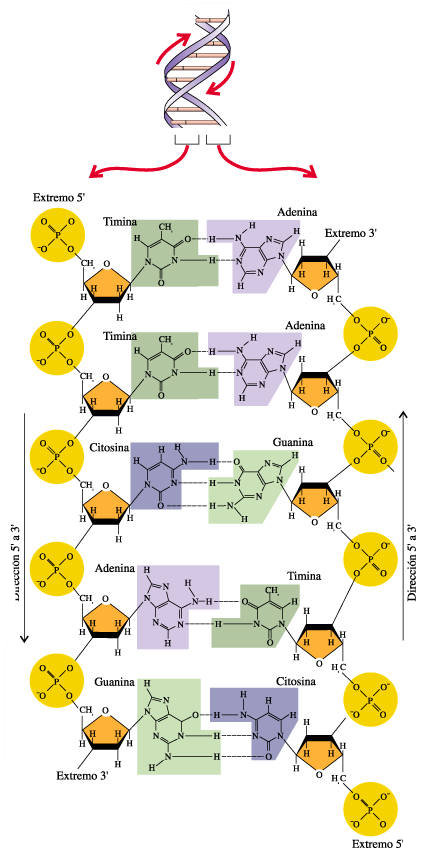
\includegraphics[width=2.2209in,height=3.2000in]{image/watson.jpg}
		\caption{Modelo estructural Watson-Crick [19].}
	\end{center}
\end{figure}	


\chapter{Clasificación de RNA}
\label{clasificacionRNA}

\begin{figure} [h]
	\begin{center}
		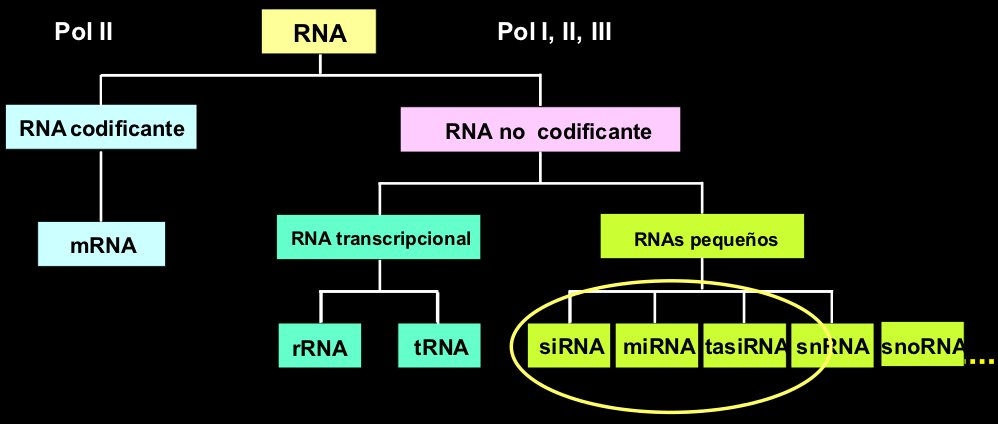
\includegraphics[width=5.8209in,height=3.0000in]{image/RNA.jpg}
		\caption{Clasificación de la molécula de RNA [20].}
			\label{rnamol}
	\end{center}
\end{figure}	

\chapter{Formato FASTA}
\label{fasta}

\par \textsc{FASTA} es un formato de archivo informático basado en texto, utilizado para representar secuencias de ácidos nucleicos, o de péptido, y en el que los pares de bases o los aminoácidos se representan usando códigos de una única letra. El formato también permite incluir nombres de secuencias y comentarios que preceden a las secuencias en sí.	

\par Una secuencia bajo formato \textsc{FASTA} comienza con una descripción en una única línea (línea de cabecera), seguida por líneas de datos de secuencia. La línea de descripción se distingue de los datos de secuencia por un símbolo ``$>$''. La palabra siguiente a este símbolo es el identificador de la secuencia, y el resto de la línea es la descripción (ambos son opcionales). No debería existir espacio entre el ``$>$'' y la primera letra del identificador. La secuencia termina si aparece otra línea comenzando con el símbolo ``$>$'', lo cual indica el comienzo de otra secuencia. 
	
\par A continuación se exhibe un ejemplo de una secuencia en tal formato:	
\begin{verbatim}
	>gi|5524211|gb|AAD44166.1| cytochrome b [Elephas maximus maximus]
	LCLYTHIGRNIYYGSYLYSETWNTGIMLLLITMATAFMGYVLPWGQMSFWGATVITNLFSAIPYIGTNLV
	EWIWGGFSVDKATLNRFFAFHFILPFTMVALAGVHLTFLHETGSNNPLGLTSDSDKIPFHPYYTIKDFLG
	LLILILLLLLLALLSPDMLGDPDNHMPADPLNTPLHIKPEWYFLFAYAILRSVPNKLGGVLALFLSIVIL
	GLMPFLHTSKHRSMMLRPLSQALFWTLTMDLLTLTWIGSQPVEYPYTIIGQMASILYFSIILAFLPIAGX
	IENY
\end{verbatim}

\section{Representación de secuencias}	
\par Cada línea de una secuencia debería tener algo menos de 80 caracteres. Las secuencia pueden corresponder a secuencias de proteínas o de ácidos nucleicos, y pueden contener huecos (o gaps) o caracteres de alineamiento.
\begin{itemize}	
	\item Los codones que codifican a un mismo aminoácido son:
	\begin{center}
		\begin{tabular}{| c | l |}
			\hline
			{\bf Aminoácido} & {\bf Nucleótidos}\\
			\hline
			\hline		
			\textcolor{blue}{Ala (A)} & GCU, GCC, GCA, GCG  \\\hline
			\textcolor{blue}{Arg (R)} & CGU, CGC, CGA, CGG, AGA, AGG  \\\hline
			\textcolor{blue}{Asn (N)} & AAU, AAC  \\\hline
			\textcolor{blue}{Asp (D)} & GAU, GAC  \\\hline
			\textcolor{blue}{Cys (C)} & UGU, UGC  \\\hline
			\textcolor{blue}{Gin (Q)} & CAA, CAG  \\\hline
			\textcolor{blue}{Glu (E)} & GAA, GAG  \\\hline
			\textcolor{blue}{Gly (G)} & GGU, GGC, GGA, GGG \\\hline
			\textcolor{blue}{His (H)} & CAU, CAC \\\hline
			\textcolor{blue}{IIe (I)} & AUU, AUC, AUA \\\hline
			\textcolor{blue}{Leu (L)} & UUA, UUG, CUU, CUC, CUA, CUG \\\hline	
			\textcolor{blue}{Val (V)} & GUU, GUC, GUA, GUG \\\hline
			\textcolor{blue}{Tyr (Y)} & UAU, UAC \\\hline
			\textcolor{blue}{Trp (W)} & UGG \\\hline
			\textcolor{blue}{Thr (T)} & ACU, ACC, ACA, ACG \\\hline
			\textcolor{blue}{Ser (S)} & UCU, UCC, UCA, UCG, AGU, AGC  \\\hline
			\textcolor{blue}{Sec (U)} & UGA  \\\hline
			\textcolor{blue}{Pro (P)} & CCU, CCC, CCA, CCG \\\hline
			\textcolor{blue}{Phe (F)} & UUU, UUC \\\hline
			\textcolor{blue}{Met (M)} & AUG \\\hline
			\textcolor{blue}{Lys (K)} & AAA, AAG \\\hline
			\textcolor{blue}{Parada (*)} & UAG, UGA, UAA \\\hline
			\textcolor{blue}{Comienzo} & AUG \\\hline	
		\end{tabular}
	\end{center}		
\end{itemize}


\section{Extensión de archivos}
	\par No hay una extensión de archivo estándar para un archivo de texto conteniendo secuencias formateadas bajo \textsc{FASTA}. Los archivos de este 	formato tienen a menudo extensiones como \textit{.fa, .mpfa, .fna, .fsa, .fas o .fasta}.


\chapter{Diseño en detalles}
\label{disenioEnDetalles}

\section{Diagrama de Clases de Remo}
\begin{figure}[!hbtp]
	\begin{center}
		\hspace*{-1.5cm}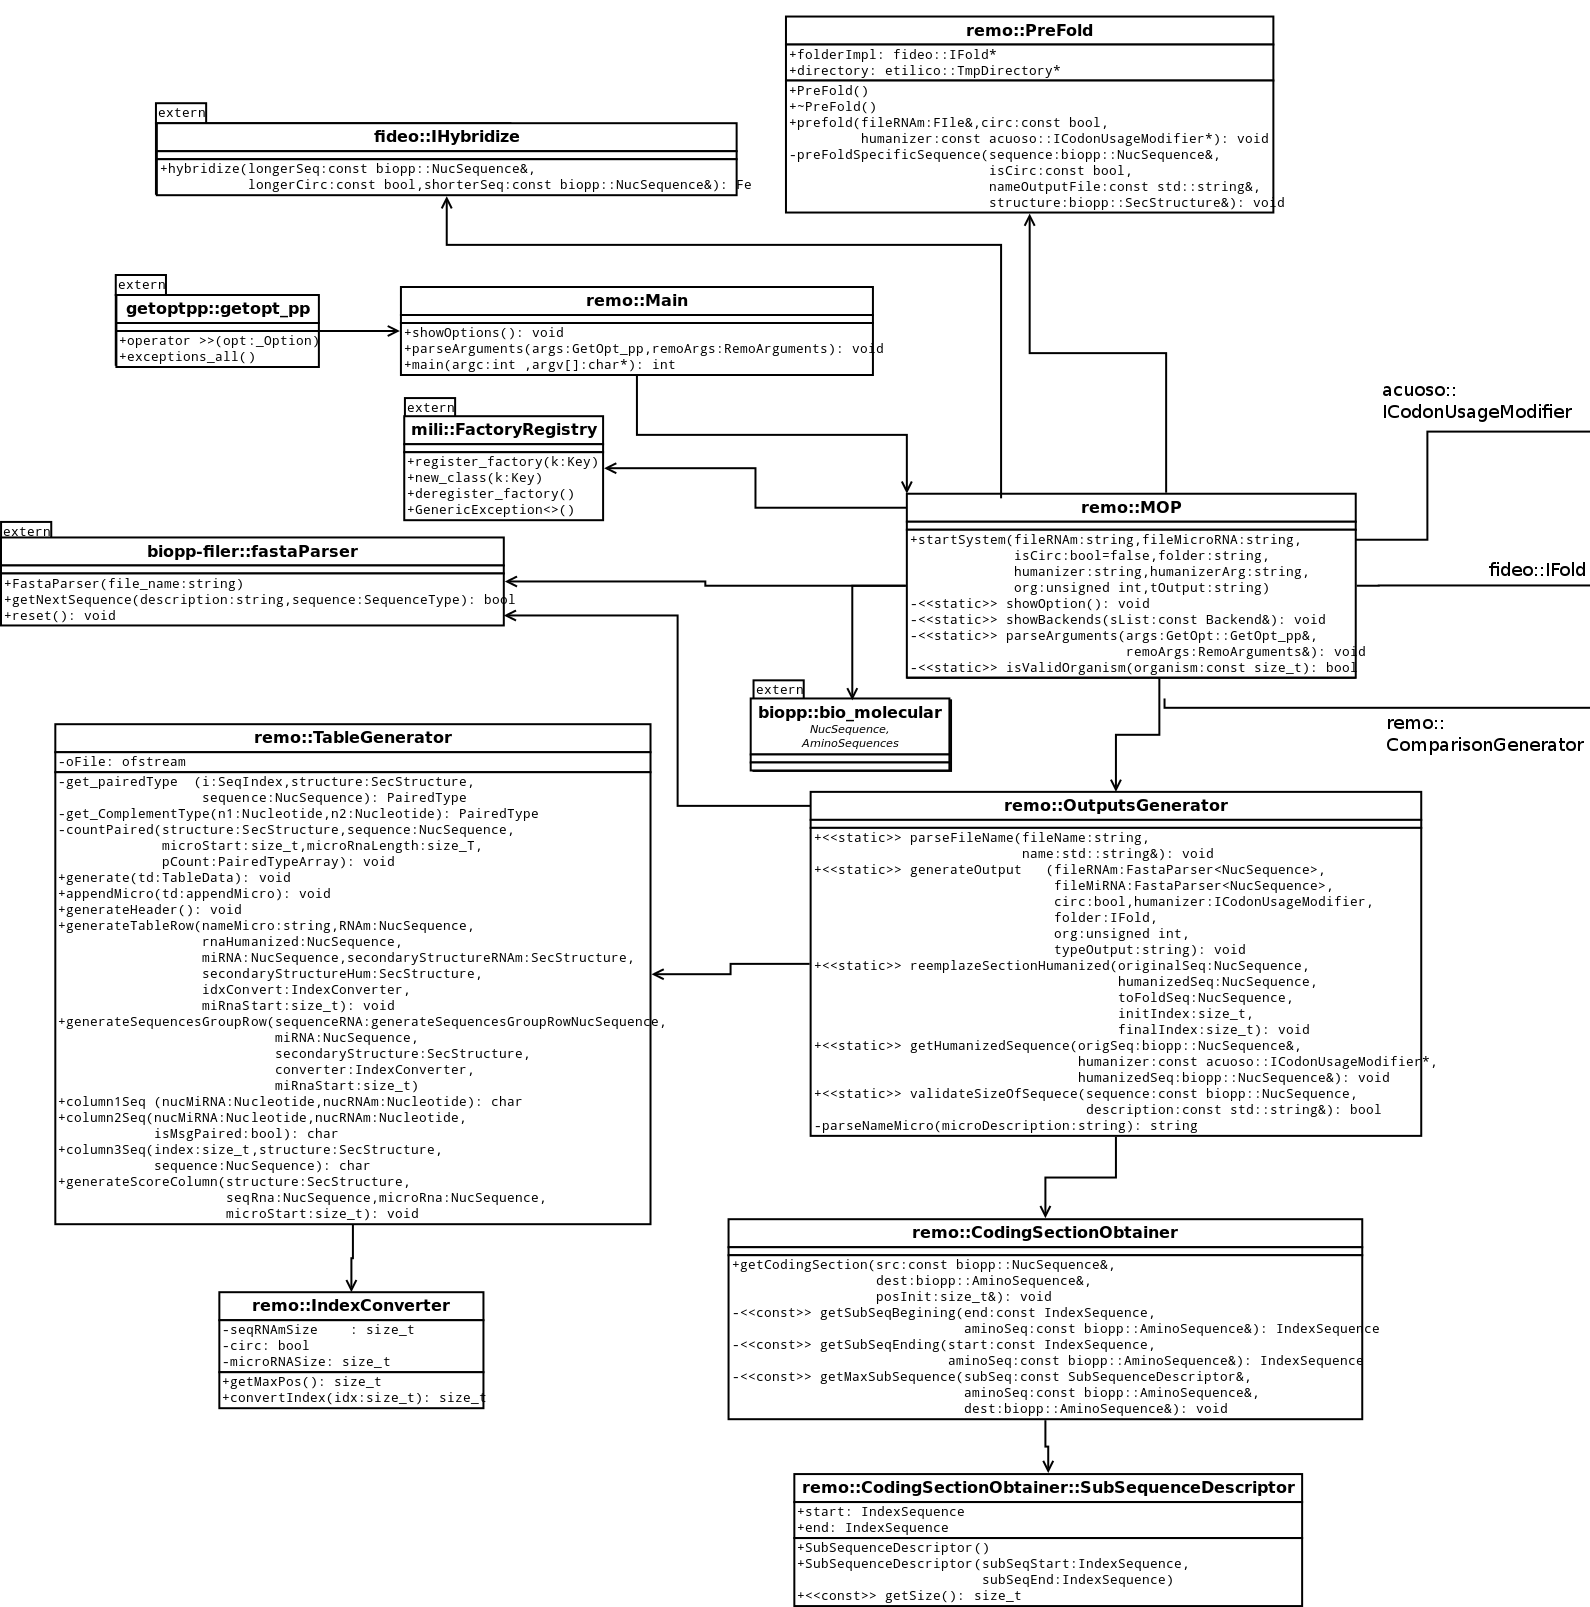
\includegraphics[width=20cm, height=17.5cm, angle=90]{image/remo1.png}
		\caption{UML - Diagrama de clases de \textbf{Remo}, parte 1 de 2 [2].}
		\label{remoDClase1}
	\end{center}
\end{figure}

\begin{figure}[!hbtp]
	\begin{center}
		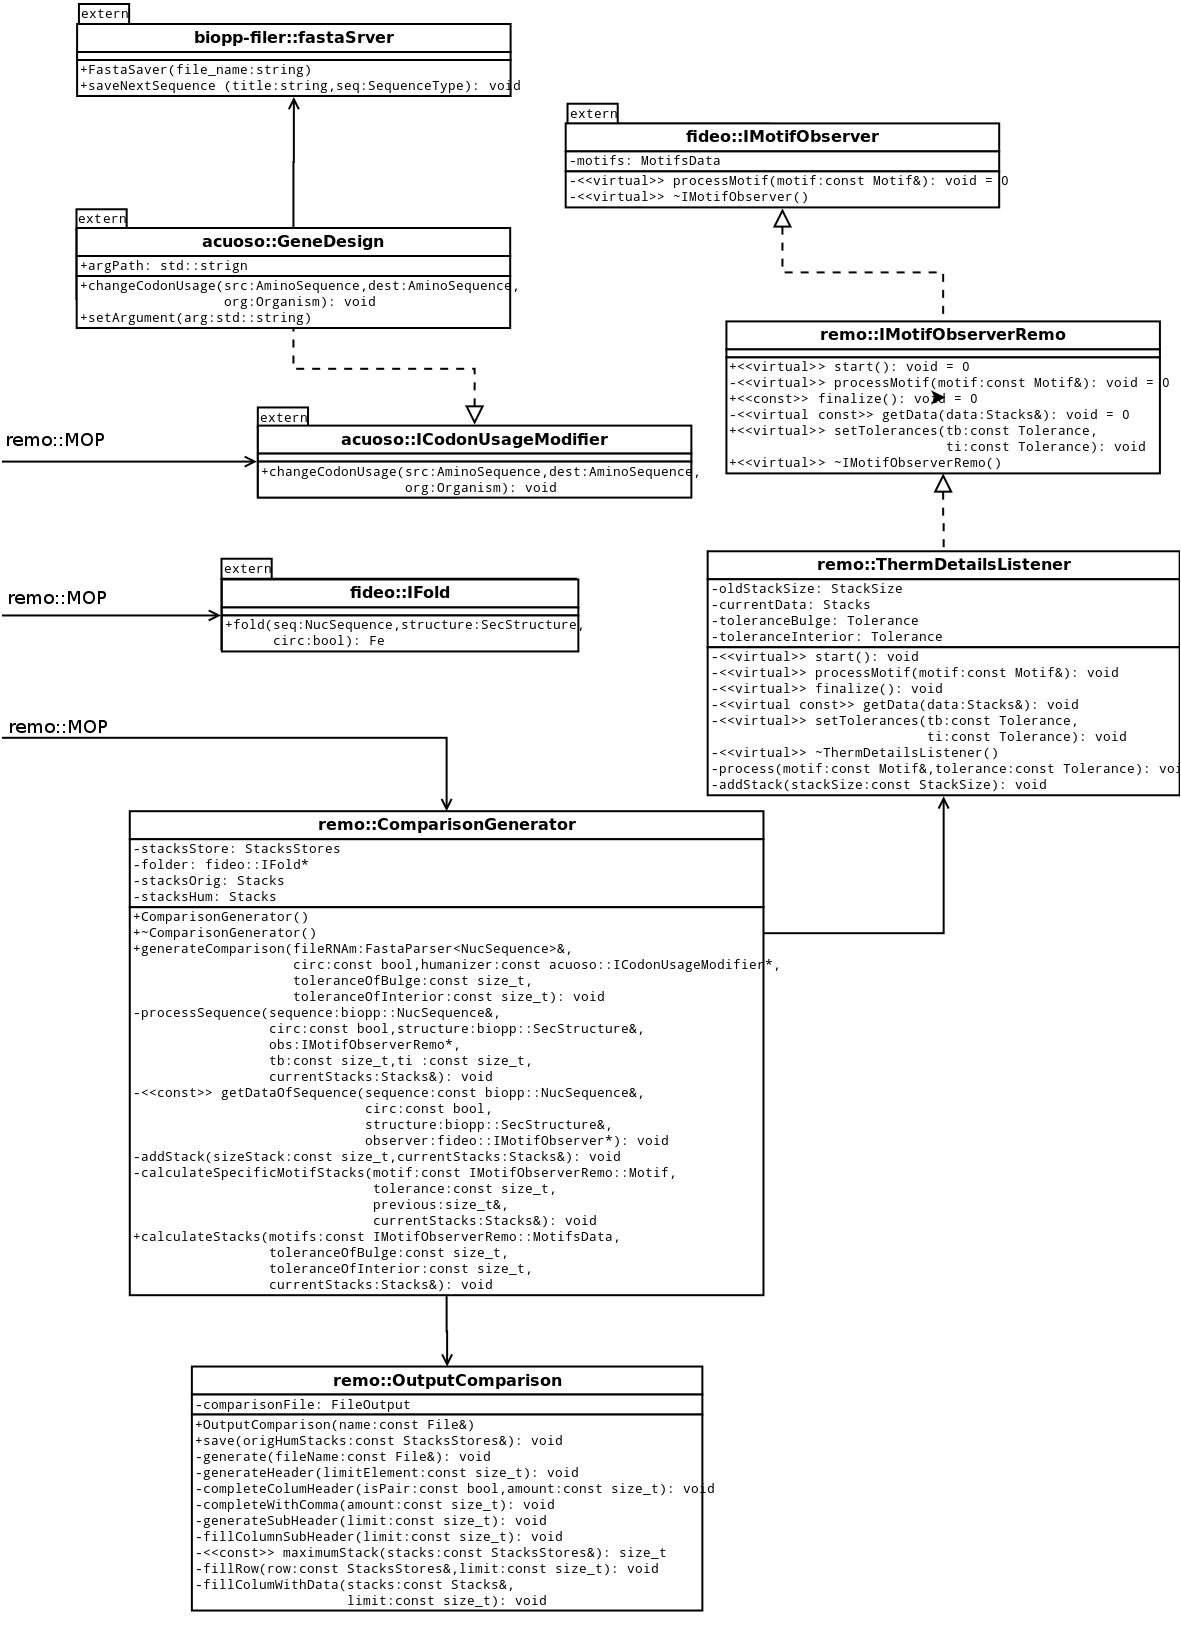
\includegraphics[width=16.5cm, height=18cm]{image/remo2.png}
		\caption{UML - Diagrama de clases de \textbf{Remo}, parte 2 de 2 [2].}
		\label{remoDClase2}
	\end{center}
\end{figure}

\section{Diagrama de Clases de Fideo}

\begin{figure}[!hbtp]
	\begin{center}
		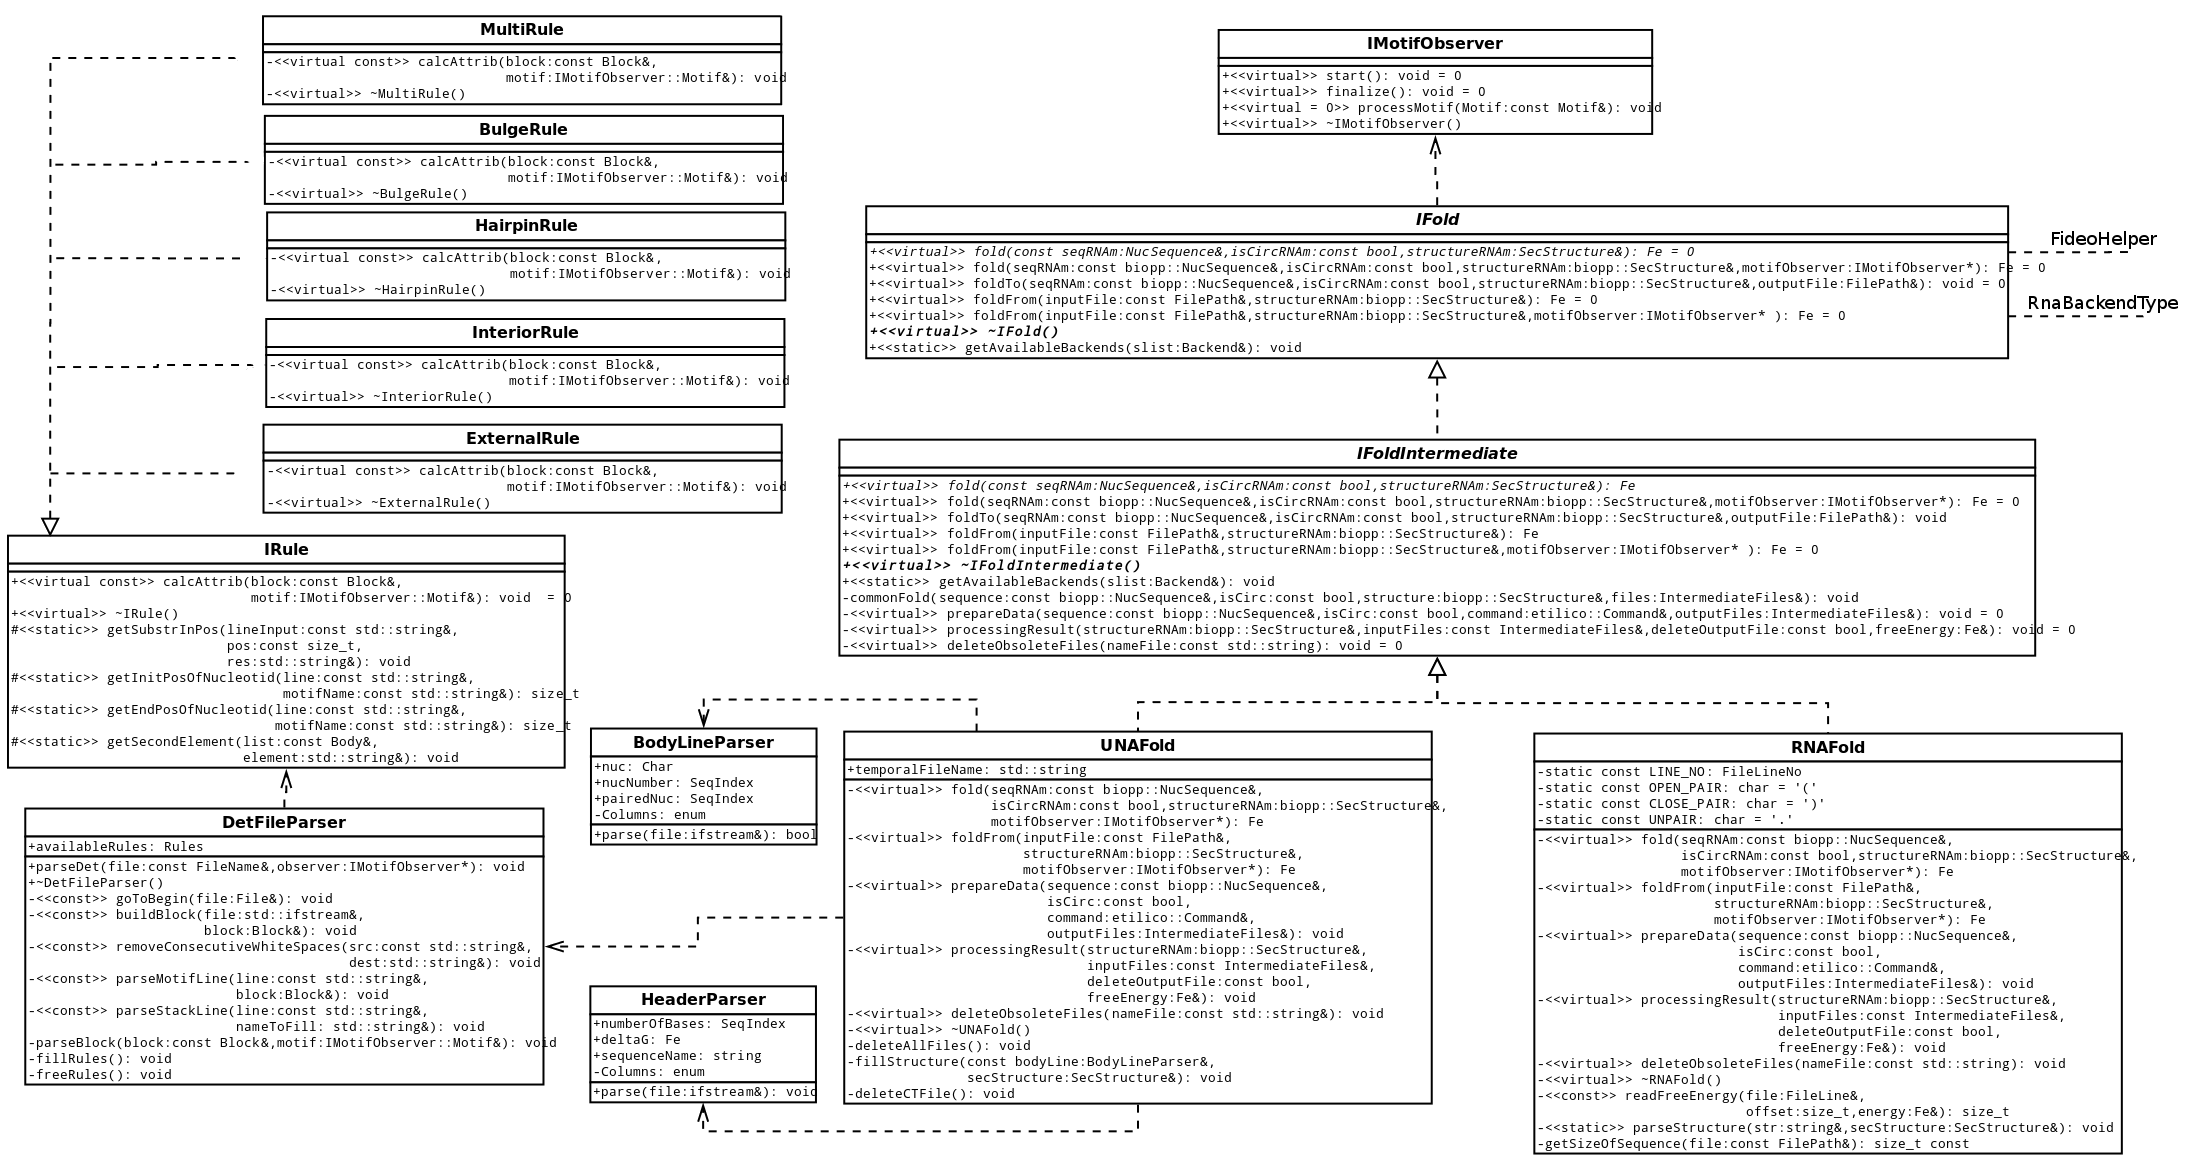
\includegraphics[width=20.5cm, height=13cm, angle=90]{image/fideoclass1.png}
		\caption{UML - Diagrama de clases de fideo, parte 1 de 2 [2].}
		\label{fideoDisenio1}
	\end{center}
\end{figure}

\begin{figure}[!hbtp]
	\begin{center}
		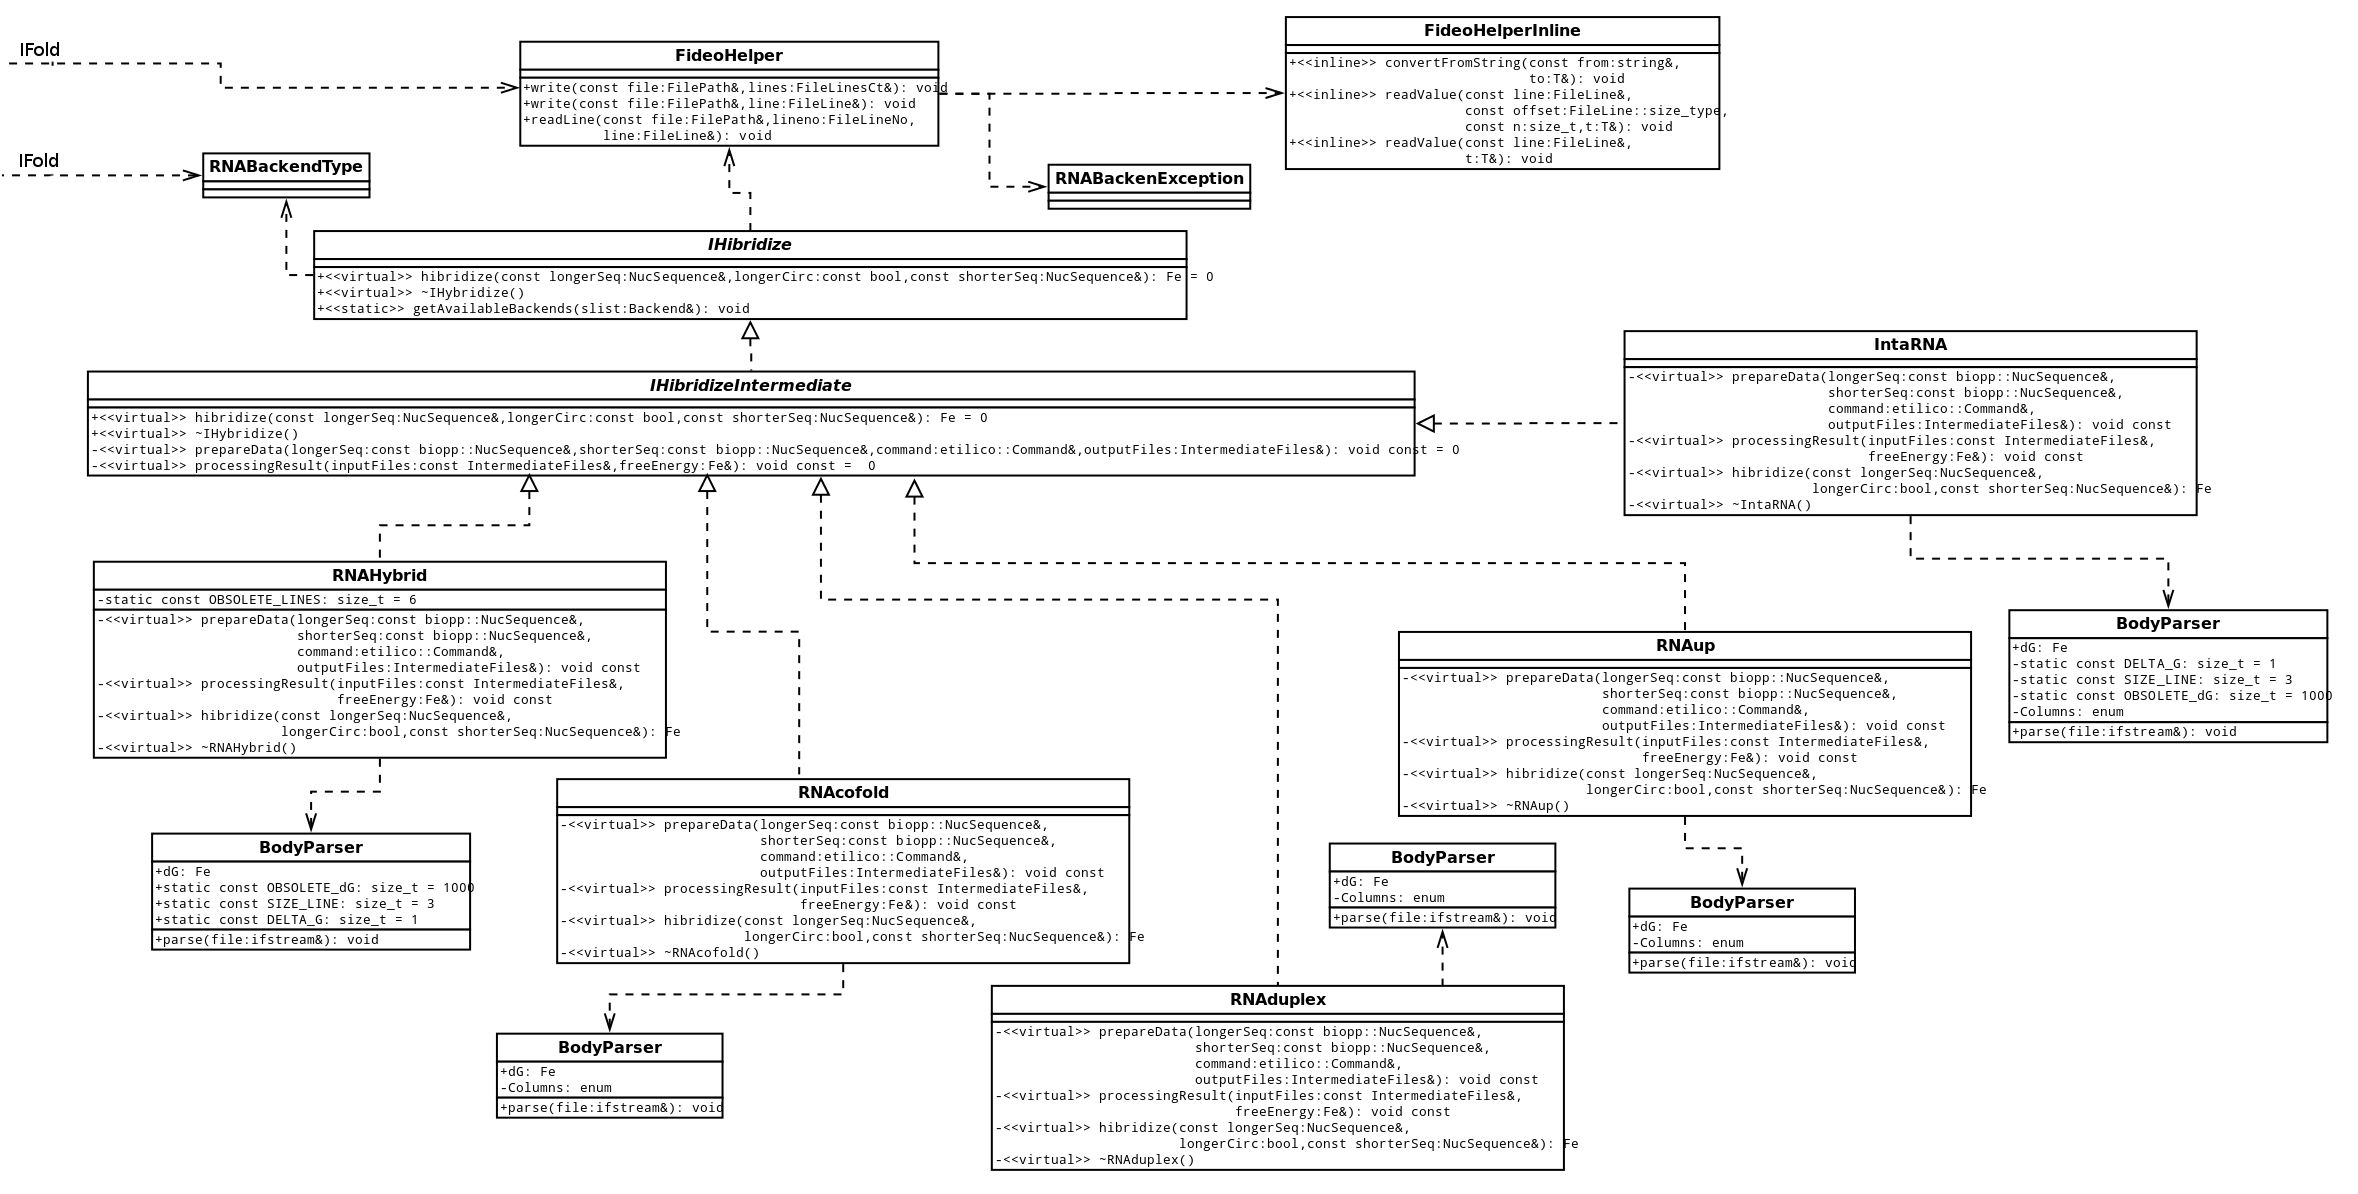
\includegraphics[width=20.5cm, height=12.5cm, angle=90]{image/fideoclass2.png}
		\caption{UML - Diagrama de clases de fideo, parte 2 de 2 [2].}
		\label{fideoDisenio2}
	\end{center}
\end{figure}
\chapter{Patrones de Diseño}
\label{patrones}

%http://www.cristalab.com/tutoriales/patrones-de-diseno-creacionales-c99932l/
\section{¿Qué son?}

En principio, se puede pensar a un patrón como una manera especialmente inteligente e intuitiva de resolver una clase de problema en particular. Según Christopher Alexander:

\begin{center}
\emph{``... un patrón describe un problema que sucede una y otra vez en nuestro entorno, y luego describe el núcleo de la solución a ese problema, de tal forma que puede utilizar esa solución un millón de veces más, sin siquiera hacerlo dos veces de la misma manera.''}
\end{center}

Los patrones de diseño~\cite{Gamma} existen independientemente de cualquier implementación particular y pueden implementarse de diversas maneras. Básicamente se clasifican según tres propósitos:
\begin{enumerate}
	\item \emph{Creacional:} tiene que ver del Cómo se puede crear un objeto. Habitualmente incluye aislar los detalles de la creación
							 del objeto, de forma que su código no dependa de los tipos de objeto que hay y por lo tanto, no es
							 necesario cambiarlo cuando se añade un nuevo tipo de objeto. Ejemplos: \emph{Singleton}, \emph{Abstract
							 Factory}, \emph{Factory Method}, entre otros.

	\item \emph{Estructural:} cuando afecta a la manera en que los objetos se conectan con otros objetos para asegurar que los cambios
							 del sistema no requieren cambiar esas conexiones. Ejemplos: \emph{Proxy}, Ejemplos: \emph{Adapter}, entre
							 otros.

	\item \emph{Comportamiento:} se emplean cuando los objetos manejan tipos particulares de acciones dentro de un programa. Éstos encapsulan procesos que quiere que se ejecuten, como interpretar un lenguaje, completar una petición, moverse a través de una secuencia  implementar un algoritmo. Ejemplos: \emph{iterator}, \emph{State}, \emph{Observer}, \emph{Strategy}, entre otros.
\end{enumerate}

\section{Patrones Empleados}

\subsection{Singleton}
\label{singleton}       
Corresponde al patrón de diseño más simple de todos, que se aplica cuando sólo se requiere una única instancia de una clase.

\begin{figure}[h!]
	\hspace*{3.5cm} 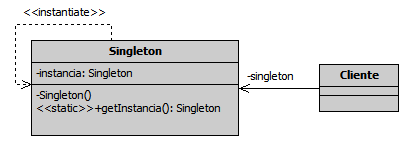
\includegraphics[scale=0.7]{image/singleton.png}
	\caption{Patrón Singleton [21].}	
\end{figure} 

\subsection{Factory Method}
\label{factoryMethod}
Consiste en definir una interfaz para crear objetos de tipo genérico permitiendo a las subclases decidir que tipo de objetos concretos crear. Es similar al \emph{Abstract Factory} pero sin el énfasis en las familias. Es un patrón muy útil dado que permite escribir aplicaciones que son más flexibles respecto de los tipos a utilizar difiriendo la creación de las instancias en el sistema a subclases que pueden ser extendidas a medida que se extiende el sistema. 

\begin{figure}[h!]
	\hspace*{1cm}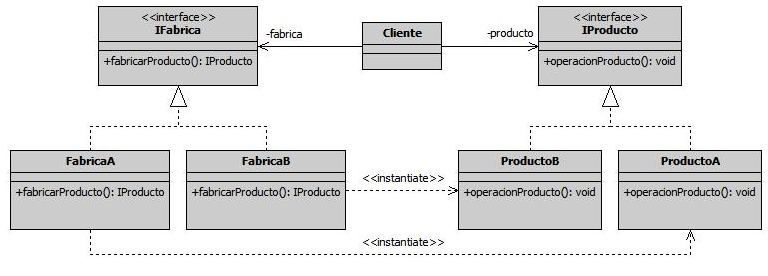
\includegraphics[scale=0.4]{image/factoryMethod.png}
	\caption{Patrón Factory Method [22].}	
\end{figure} 

\begin{verbatim}
struct Speaker
{
    virtual void saySomething() = 0;
    virtual ~Speaker(){}
};

class Hello: public Speaker
{
    virtual void saySomething();
};

void Hello::saySomething()
{
    std::cout << "Hello" << std::endl;
}

REGISTER_FACTORIZABLE_CLASS(Speaker, Hello, std::string, "Hello");

class Goodbye: public Speaker
{
    virtual void saySomething();
};

void Goodbye::saySomething()
{
    std::cout << "Goodbye" << std::endl;
}

REGISTER_FACTORIZABLE_CLASS(Speaker, Goodbye, std::string, "Goodbye");

int main()
{
	Speaker* speaker = mili::FactoryRegistry<Speaker, std::string>::new_class("Hello");
	speaker->saySomething();
	delete speaker;
	return 0;
}

Output: Hello
\end{verbatim}

\subsection{Observer}
\label{observer}
Define una dependencia del tipo $1->N$ entre objetos, de tal forma que cuando el objeto cambia de estado, todos sus objetos dependientes son notificados automáticamente. Los objetos observadores se añadan a una lista de objetos, y el objeto observado notificará el cambio a todos los objetos de esta lista cuando se produzca el cambio. Básicamente se aplica cuando se necesita consistencia entre clases relacionadas, pero con independencia, es decir, con un bajo acoplamiento. 

\begin{figure}[h!]
	\centering
		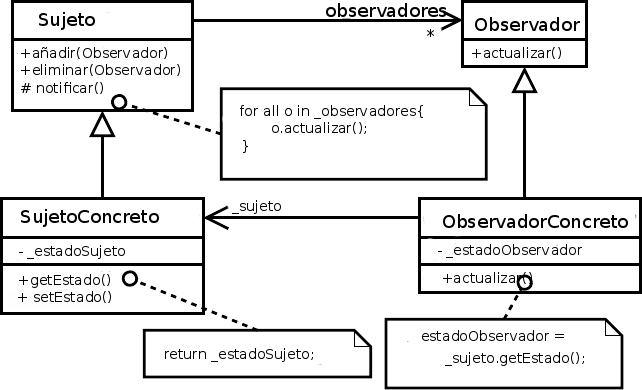
\includegraphics[scale=0.4]{image/observer.png}
	\caption{Patrón Observer [23].}
\end{figure} 	

Un funcionamiento básico de este patrón se exhibe en la figura ~\ref{observerDiagram}.

\begin{figure}[h!]
	\centering
		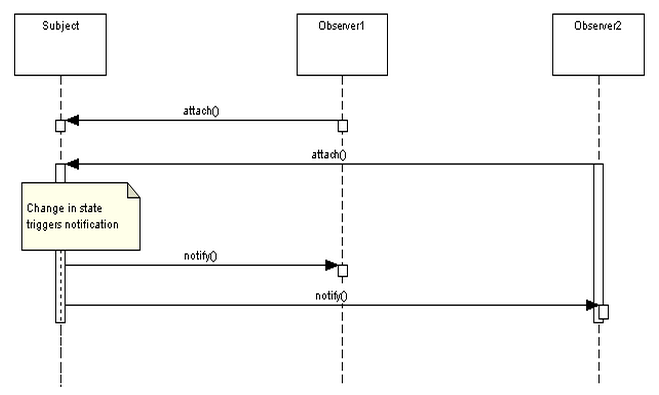
\includegraphics[scale=0.5]{image/observerDiagram.png}
	\caption{Diagrama de Secuencias Observer [24].}
	\label{observerDiagram} 
\end{figure}

\subsection{Template Method}
\label{templateMethod}

\par Corresponde a un patrón de diseño de comportamiento. Este tipo de patrón ayuda a resolver problemas de interacción entre clases y objetos. Surge de la necesidad de extender determinados comportamientos dentro de un mismo algoritmo por parte de diferentes entidades. Es decir, diferentes entidades tienen un comportamiento similar pero que difiere en determinados aspectos puntuales en función de la entidad concreta. Una posible solución consiste en copiar el algoritmo en cada de las diferentes entidades cambiando la parte concreta en la que difieren, aunque tiene una consecuencia negativa ya que se genera código duplicado.  
\par La solución que propone el mencionado patrón es abstraer todo el comportamiento que comparten las entidades en una clase (abstracta) de la que, posteriormente, extenderán dichas entidades. Esta superclase definirá un método que contendrá el esqueleto de ese algoritmo común (método plantilla) y delegará determinada responsabilidad en las clases hijas, mediante uno o varios métodos abstractos que deberán implementar. La estructura del patrón se exhibe en la figura~\ref{templateMethod}.

\begin{figure}[h!]
	\centering
		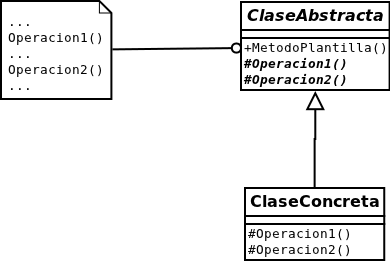
\includegraphics[scale=0.5]{image/templateMethod.png}
	\caption{Template Method [25].}
	\label{} 
\end{figure}

\par Es un patrón que se adecuada cuando contamos con un algoritmo con varios pasos que no cambian, de modo que dichos pasos invariantes serían implementados en una superclase, dejando la implementación de los pasos que cambian para las subclases. A continuación se muestra un ejemplo del patrón en pseudo-código:

\begin{lstlisting}[basicstyle=\tt, frame=trBL, tabsize=4,fontadjust=true]
class Base
{
  public:
    void execute()
    {
        a();
        ph1();
        c();
        ph2();
        e();
    }
  private:
    void a() { ... }
    void c() { ... }
    void e() { ... }    
    virtual void ph1() = 0;
    virtual void ph2() = 0;
};

class One: public Base
{
    /*virtual*/void ph1() { ... }
    /*virtual*/void ph2() { ... }    
};

class Two: public Base
{
 	/*virtual*/void ph1() { ... }
    /*virtual*/void ph2() { ... }       
};
	
\end{lstlisting}
\hspace*{2cm}\caption{Código D.1: Pseudo-código patrón Template Method.}

\subsection{Mediator}
\label{mediator}
\par El patrón de diseño \emph{Mediator} está considerado como un patrón de comportamiento. Básicamente encapsula la comunicación entre muchas clases mediante un objeto mediador.

\par En POO seguramente se tendrán que crear un montón de clases que interactúan entre sí. Si no se aplican ciertos principios, cada objeto dependerá de muchos otros. Con el fin de evitar marcos acoplados, surge el patrón mediador para facilitar la interacción entre los objetos de una manera en la que cada objeto no es conscientes de la existencia de otros objetos.

\par En la figura~\ref{mediador} se exhibe un ejemplo de uso presente patrón.

\begin{figure}[h!]
	\centering
		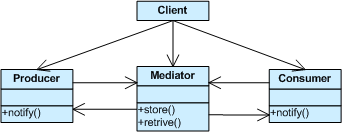
\includegraphics[scale=0.7]{image/mediador.png}
	\caption{Ejemplo patrón Mediator [18].}
	\label{mediador} 
\end{figure}

\chapter{Detalles de FuD}
\label{detFud}

\par \textbf{FuD} fue implementado empleando usando un esquema \emph{Divide \& Conquer} donde el procesamiento es llevado a cabo por los nodos procesadores. ``Divide'' cuando se realiza la división de un trabajo en una unidad de trabajo. ``Conquer'' al incorporar los resultados de una unidad de trabajo.

\section{Diseño}
A continuación se describe brevemente cada una de las capas que constituyen el framework.

\subsection{Application Layer (L3)} 
\par Básicamente proporciona los componentes que contienen todos los aspectos del dominio del problema a resolver. Estos aspectos incluyen todas las definiciones de los datos usados y su manipulación correspondiente, como así también todos los algoritmos relevantes para la solución al problema en general. 

\par Es necesario que del lado del servidor se implemente la aplicación principal, la cual hará uso de una simple interfaz en la abstracción de un trabajo distribuible permitiendo así codificar la estrategia de distribución de trabajos. Del lado cliente, solo se necesita implementar los métodos encargados de realizar las computaciones indicadas por una unidad de trabajo.

\subsection{Job Management Layer (L2)} %manejador de trabajo
\par Esta capa permite manejar los trabajos que se desean distribuir como así también generar las unidades de trabajo que serán entregadas a los clientes para su procesamiento. Estas unidades de trabajo llegan a su cliente correspondiente gracias a la capa más baja, encargada de la distribución. Una vez finalizado el procesamiento, se informa que todo ha terminado y otorga los resultados a la capa superior.

\subsection{Distributing Middleware Layer (L1)} %comunicación
\par En esta capa existe el único vínculo real entre clientes y servidor. La responsabilidad principal es manejar los clientes conectados al servidor y llevar a cabo los procedimientos de comunicación entre ambos.

\par Las implementaciones concretas de este nivel son variables y están determinadas por el middleware a utilizar, por ejemplo \textsc{Boost.Asio}\footnote{\url{http://www.boost.org/doc/libs/1\_4\_00/doc/html/boost\_asio.html}}, \textsc{MPI}\footnote{\url{http://www.mcs.anl.gov/research/projects/mpi/}} o \textsc{BOINC}\footnote{\url{http://boinc.berkeley.edu/}}. 
		
\par Actualmente, \emph{FuD} cuenta con dos capas más, conocidas como \emph{FuD-RecAbs} y \emph{FuD-CombEng}. Estas capas no se describen dado que sólo se empleará \textbf{FuD} original, para mayor información consultar \url{fud.googlecode.com.}

\end{document}